%!TEX root = ../../../adrien_gomar_phd.tex
\chapter{Isolated high-speed CROR configuration}
\label{cha:dream_hs_isolated}

\chabstract{To further assess the proposed
multi-frequential harmonic balance method along
with a weak-coupling approach, a more demanding
case is studied, namely a high-speed configuration.
The number of harmonics required to compute such a
configuration is shown to be higher than the 
low-speed configuration. The unsteady rigid
computations are analyzed and aeroelastic
simulations are then launched, showing that 
the proposed approach is robust enough to 
assess such configurations.}

\newpage

\section{Presentation of the case}
\label{sec:dream_hs_presentation}
%!TEX root = ../../../adrien_gomar_phd.tex




\section{Numerical setup}
\label{sec:dream_hs_numerical}
%!TEX root = ../../../adrien_gomar_phd.tex

The same topology and number of grid points is used to
mesh this high-speed configuration. The reader is referred to 
Sec.~\ref{sec:dream_ls_numerical} for detailed information.

\paragraph{Influence of the spatial discretization}
\label{sub:dream_hs_spatial_discretization}

To assess the different spatial scheme for this high-speed
CROR configuration, the same exercise as done in 
Sec.~\ref{sub:dream_ls_spatial_discretization} is made below.
The same four schemes are evaluated based 
on the convergence of the computation
and the convergence of the integrated 
results (similarity coefficients).
For the \citet{Jameson1981} scheme, the artificial viscosities
are chosen as follow: $\kappa_2 = 1.0$ as the configuration is likely to 
see shocks and $\kappa_4 = 0.016$. We will see that the computation converges
with this low $\kappa_4$ coefficient. Therefore, only this coefficient
will be tested.

The convergence of the computations using the four spatial schemes
is shown in Fig.~\ref{fig:DREAM_HS_RESIDUALS_PPT}. The convergence is good
for all the spatial schemes. In fact, more than five order of magnitude
is lost on the residuals.
\begin{figure}[htb]
  \centering
  \includegraphics*[width=0.50\textwidth]{SPACE_SCHEME_DIFF_HS_RESIDUALS.pdf}
  \caption{High-speed isolated configuration: convergence 
  of steady computations using different spatial schemes.}
  \label{fig:DREAM_HS_RESIDUALS_PPT}
\end{figure}

The values of the similarity coefficients obtained with
all the spatial schemes is reported in 
Fig.~\ref{fig:dream_hs_space_scheme_coeff}. The values are
given as a ratio over the Roe~2 values. The first order
upwind scheme (Roe~1) give similarity coefficients that are
several percent lower than the Roe~2 value. The other schemes
give results that are less than 1\% close, therefore and for
consistence with the approach retained for the LS configuration
the Roe~2 scheme is chosen for the following results.
\begin{figure}[htb]
  \centering
  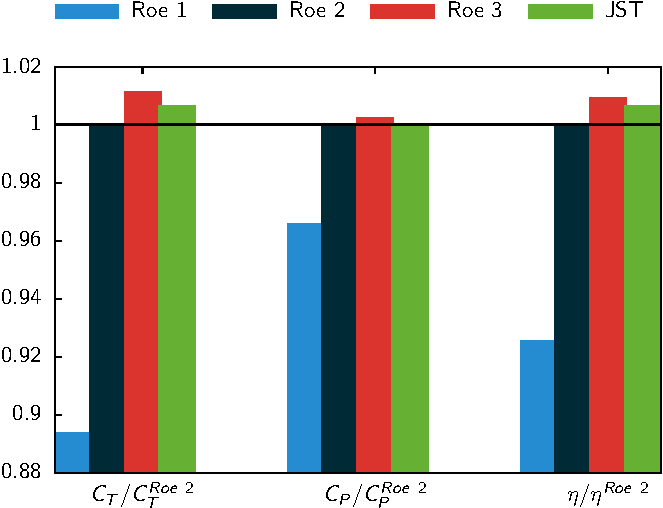
\includegraphics[width=.5\textwidth]{SPACE_SCHEME_DIFF_HS_COEFF.pdf}
  \caption{High-speed isolated configuration: convergence of 
  similarity coefficients using different spatial schemes.}
  \label{fig:dream_hs_space_scheme_coeff}
\end{figure}



\section{Steady results}
\label{sec:dream_hs_steady_results}
%!TEX root = ../../../adrien_gomar_phd.tex

\subsection{Analysis of the convergence}
\label{sub:dream_hs_steady_conv}

The convergence of the simulation is obtained 
after one thousand iterations for both
the residuals and the similarity coefficients 
(Figure~\ref{fig:dream_HS_convergence_roe2}). More than
five order of magnitude is obtained for the residuals and
the similarity coefficients are stabilized starting below
$1,000$ iterations. According to \citet{Casey2000},
this means that the steady simulation is converged.
\begin{figure}[htp]
  \centering
  \subfigure[residuals]{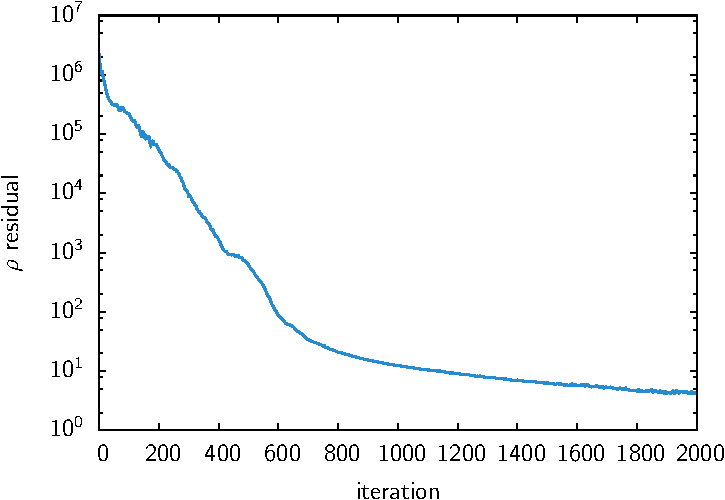
\includegraphics[width=.35\textwidth]{DREAM_HS_RESIDUALS_PPT.pdf}}
  \subfigure[$C_T$]{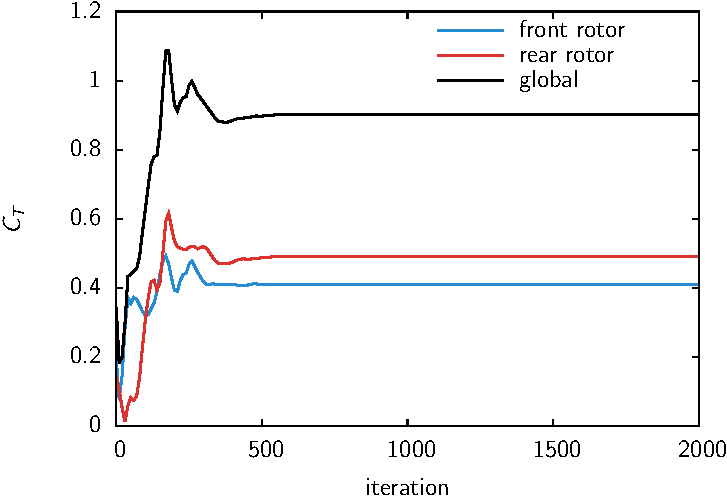
\includegraphics[width=.35\textwidth]{DREAM_HS_FORCES_CT_PPT.pdf}}
  \subfigure[$C_P$]{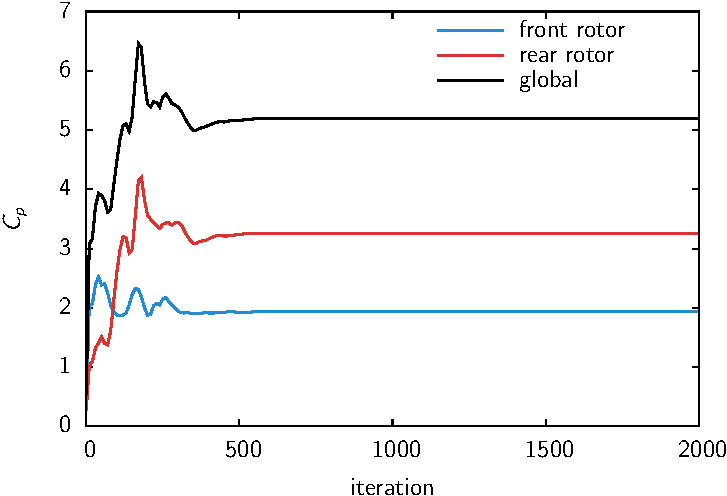
\includegraphics[width=.35\textwidth]{DREAM_HS_FORCES_CP_PPT.pdf}}
  \subfigure[$\eta$]{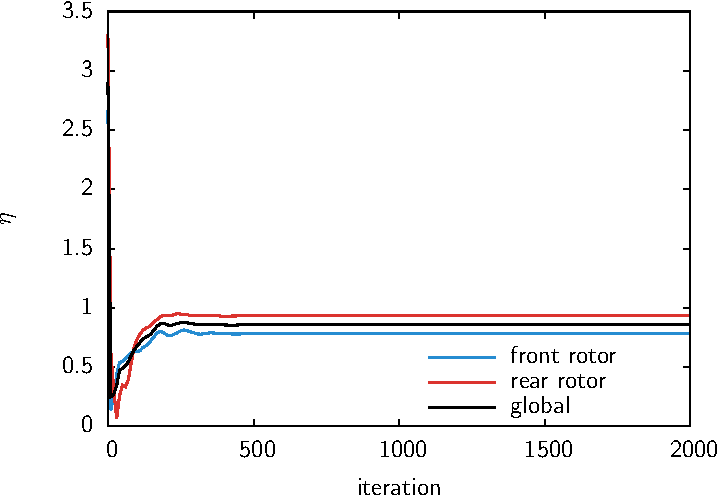
\includegraphics[width=.35\textwidth]{DREAM_HS_FORCES_ETA_PPT.pdf}}
  \caption{High-speed isolated configuration: convergence of the steady
  computation.}
  \label{fig:dream_HS_convergence_roe2}
\end{figure}

\subsection{Similarity coefficients}
\label{sub:dream_hs_sim_coeff}

The similarity coefficients are representative of a cruise
propeller (see Eq.~\eqref{eq:estimation_sim_coeff}). 
Firstly, the thrust is higher
on the rear rotor than on the front rotor, even though it is
relatively well distributed. Bare in mind that the rear rotor
similarity coefficient is normalized by the front rotor diameter. Therefore, 
the thrust produced by the rear rotor is larger than the one of the front rotor, 
relatively to its diameter. 
Secondly, the power coefficient is similar for both the front and the
rear rotor. As the power coefficient represents the mechanical input
given to flow, this means that the mechanical distribution is 
well distributed, which is a design wish.
\begin{table}[htp]
  \ra{1.3} \centering
  \begin{tabular}{ccc|cccccc}
    \toprule
    $C_T$ & $C_P$ & $\eta$ & $C_{T_f}$ & $C_{P_f}$ & $\eta_f$ & $C_{T_r}$ & $C_{P_r}$ & $\eta_r$ \\
    \midrule
    0.9017 & 3.8485 & 0.8577 & 0.4105 & 1.9262 & 0.7801 & 0.4912 & 1.9223 & 0.9354 \\
    \bottomrule
  \end{tabular}
  \caption{High-speed isolated configuration: similarity coefficients.}
  \label{tab:dream_HS_sim_coeff}
\end{table}

\subsection{Radial profiles}
\label{sub:dream_hs_radial_profiles}

Radial profiles are computed on the steady results and 
reported in Fig.~\ref{fig:dream_HS_radial_profiles}.

The absolute Mach number increases from its inflow
value ($M_a = 0.73$) up to around $M_a=0.81$. This represents
a 10\% 

\begin{figure}[htp]
  \centering
  \subfigure[absolute Mach number]{
    \label{fig:dream_HS_radial_profiles_ma}
    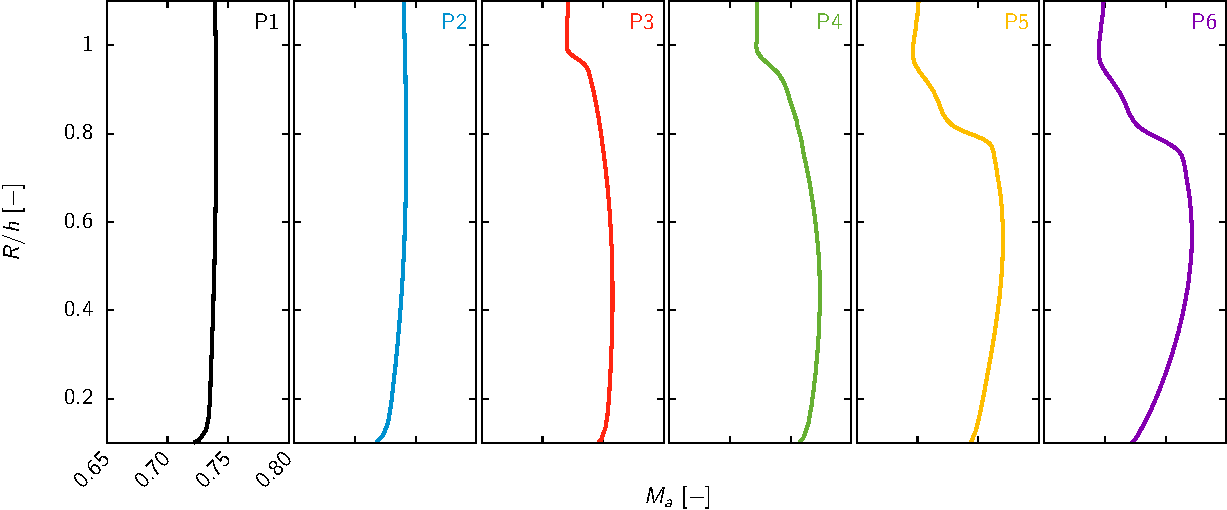
\includegraphics[width=.72\textwidth]{DREAM_HS_RANS_AZI_MEAN_PPT_macha.pdf}}
  \subfigure[absolution flow angle]{
    \label{fig:dream_HS_radial_profiles_alpha}
    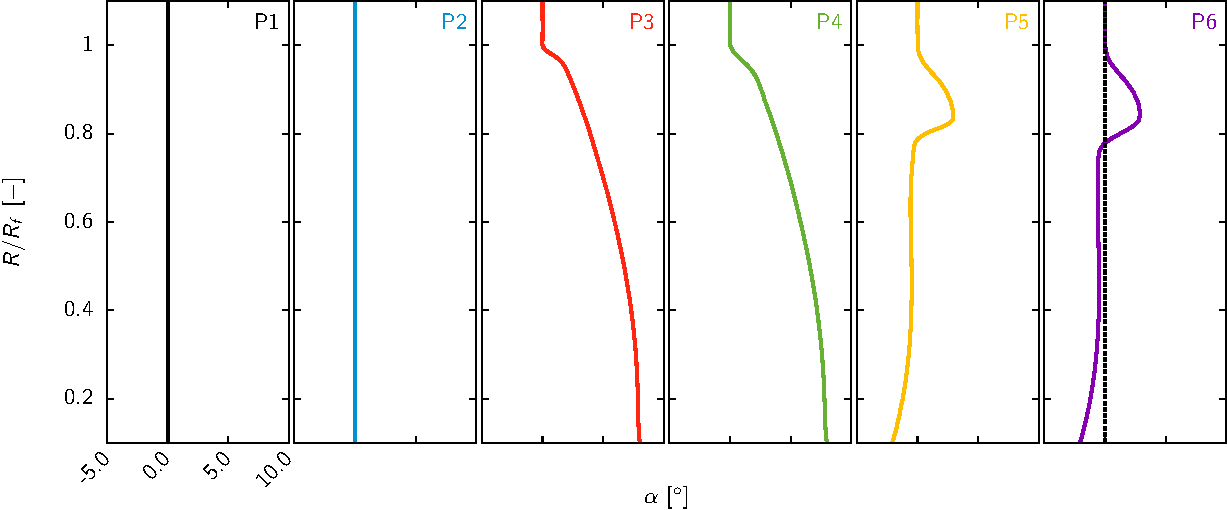
\includegraphics[width=.72\textwidth]{DREAM_HS_RANS_AZI_MEAN_PPT_alpha.pdf}}
  \caption{High-speed isolated configuration: radial profiles.}
\end{figure}
\setcounter{figure}{\value{figure}-1}
\begin{figure}[htp]
  \centering
  \setcounter{subfigure}{3}
  \subfigure[static pressure]{
    \label{fig:dream_HS_radial_profiles_ps}
    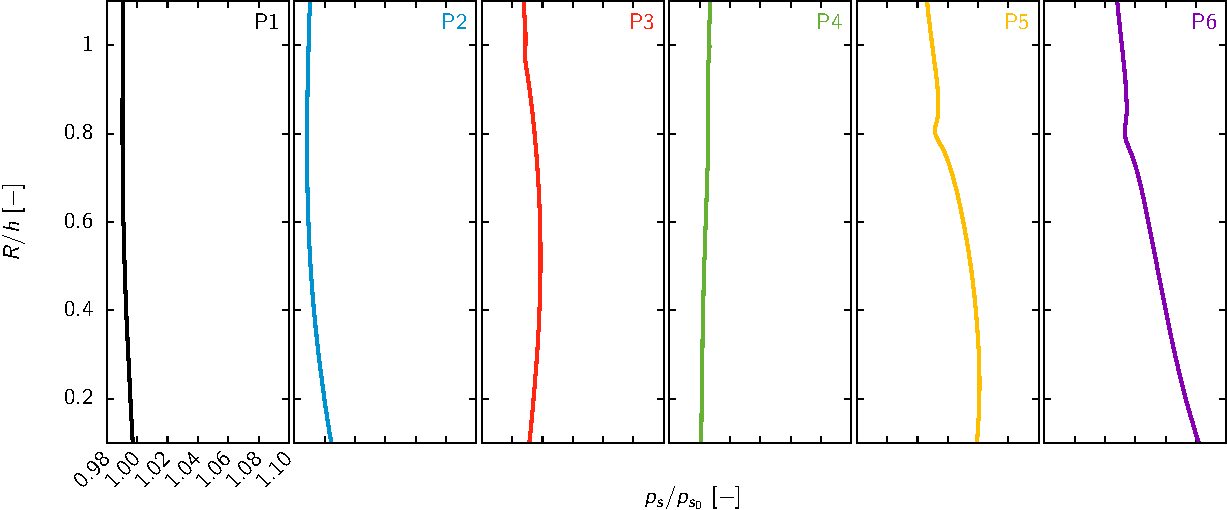
\includegraphics[width=.72\textwidth]{DREAM_HS_RANS_AZI_MEAN_PPT_ps.pdf}}
  \subfigure[stagnation pressure]{
    \label{fig:dream_HS_radial_profiles_pi}
    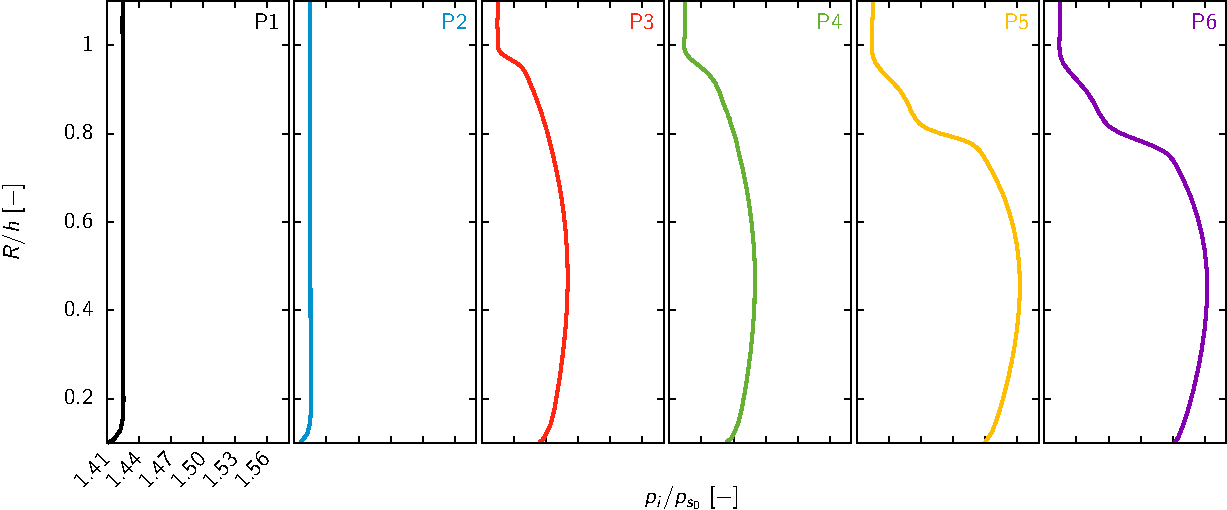
\includegraphics[width=.72\textwidth]{DREAM_HS_RANS_AZI_MEAN_PPT_pi.pdf}}
  \subfigure[stagnation temperature]{
    \label{fig:dream_HS_radial_profiles_ti}
    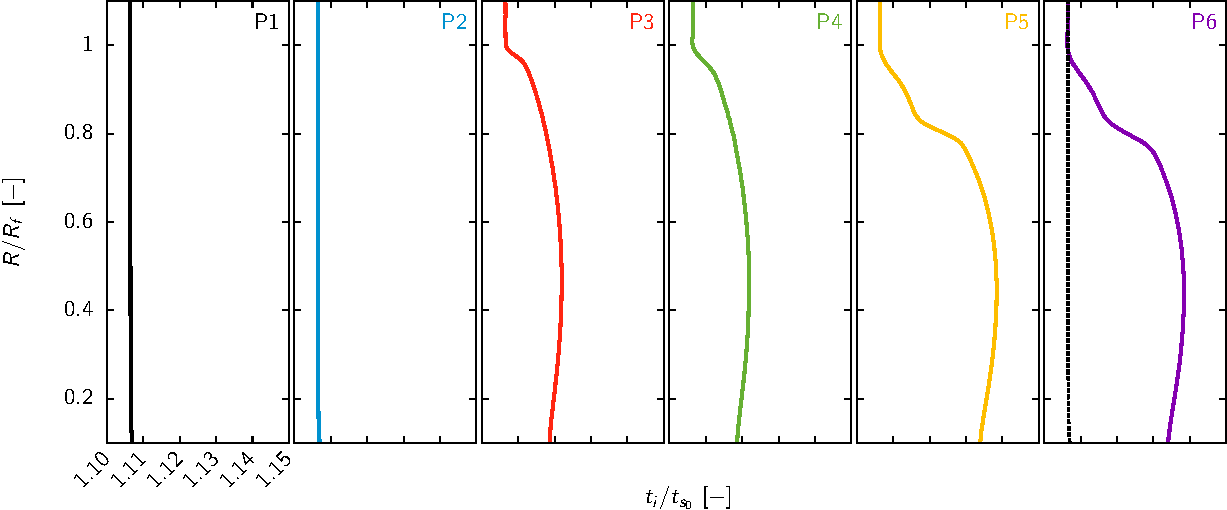
\includegraphics[width=.72\textwidth]{DREAM_HS_RANS_AZI_MEAN_PPT_ti.pdf}}
  \caption{High-speed isolated configuration: radial profiles (contd.).}
  \label{fig:dream_HS_radial_profiles}
\end{figure}

\subsection{Flow field around the blades}
\label{sub:dream_hs_blades}


\begin{figure}[htp]
 \centering
 \begin{tabular}{rccc}
   & $-k_p$ front rotor
   & $-k_p$ rear rotor
   & relative Mach number\\
   \rotatebox{90}{\qquad\qquad 25~\%} 
   & 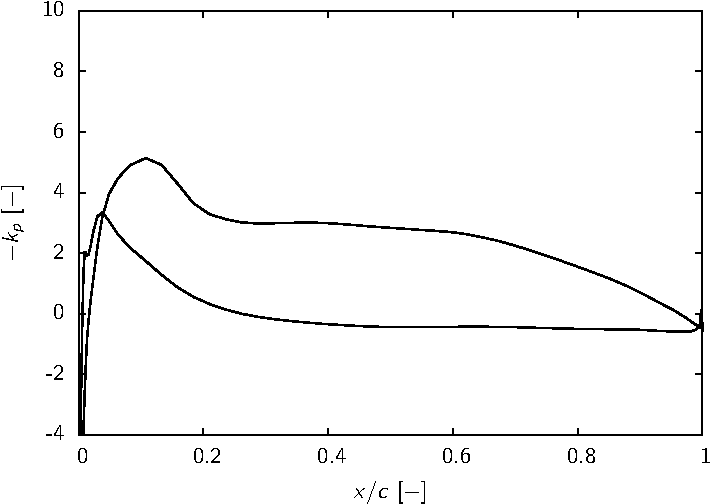
\includegraphics[width=0.28\textwidth]{DREAM_HS_KP_25_FRONT_PPT.pdf}
   & 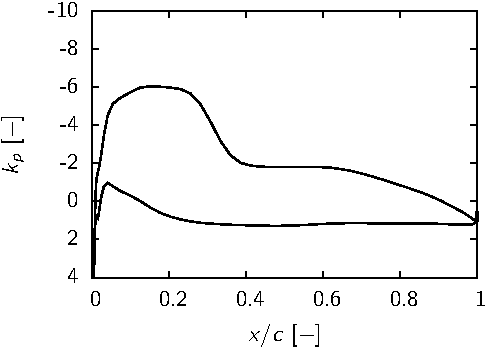
\includegraphics[width=0.28\textwidth]{DREAM_HS_KP_25_REAR_PPT.pdf}
   & 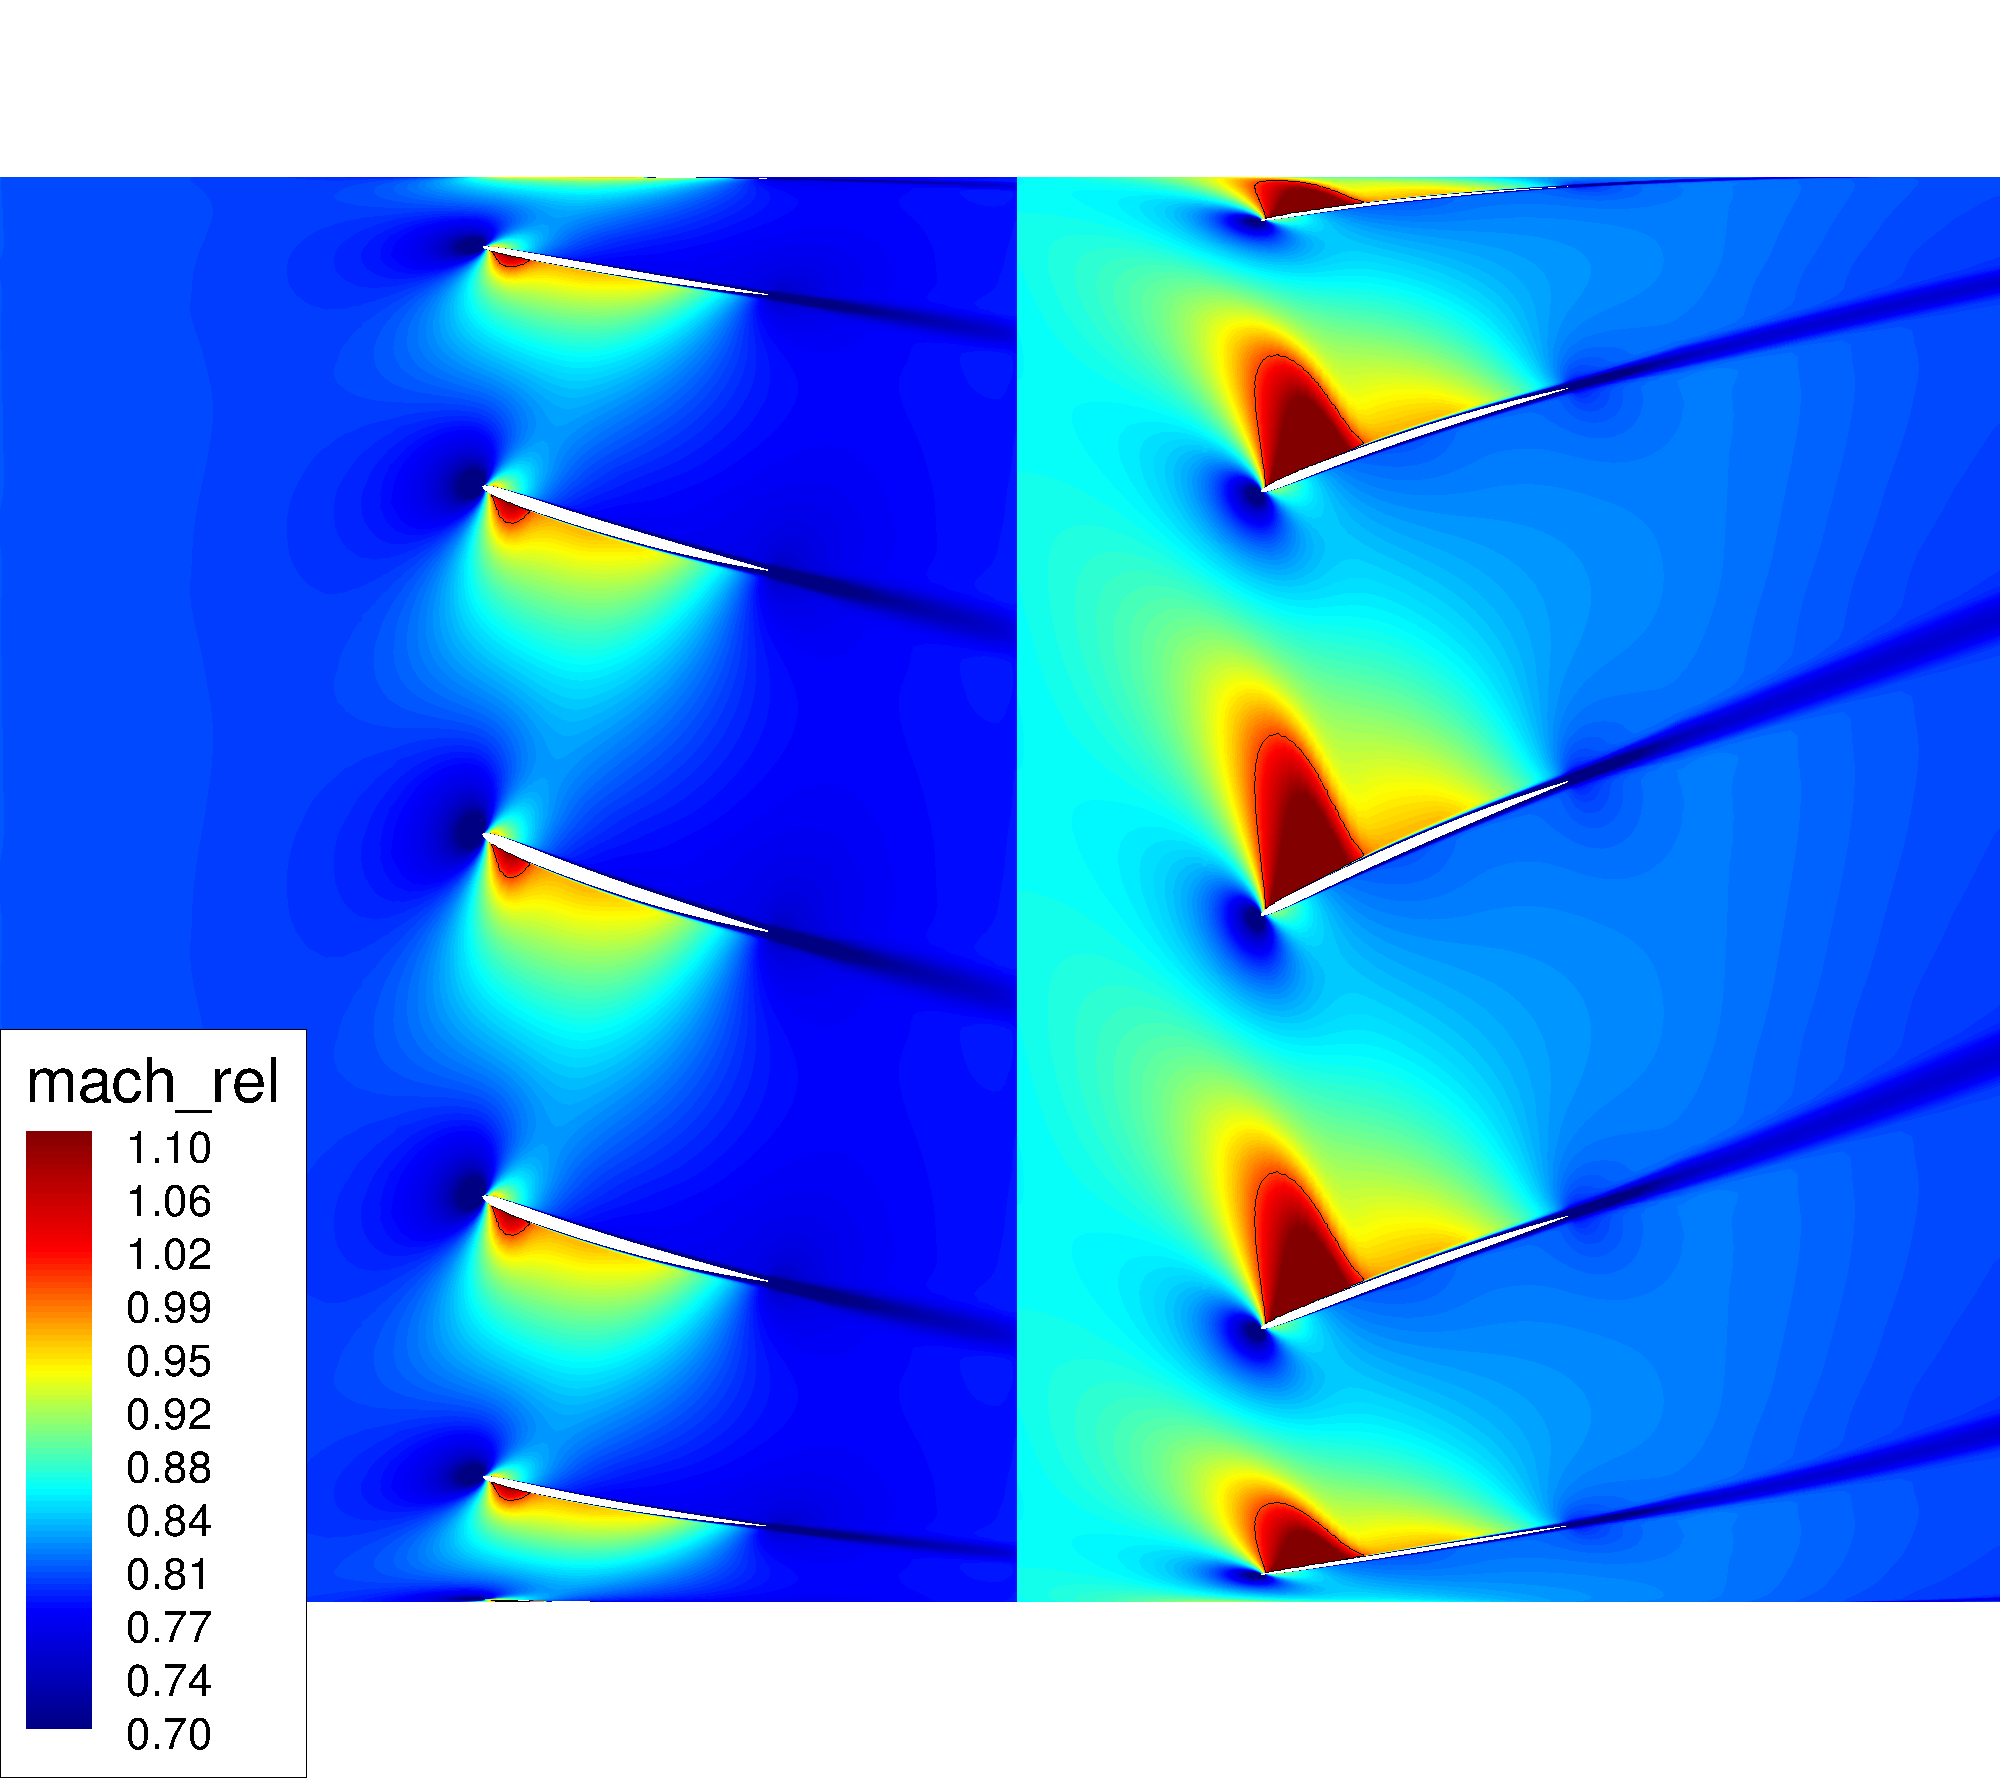
\includegraphics[width=0.28\textwidth]{DREAM_HS_RANS_roe2_sa_slice_r_25_mach_rel.png}\\
   \rotatebox{90}{\qquad\qquad 50~\%} 
   & 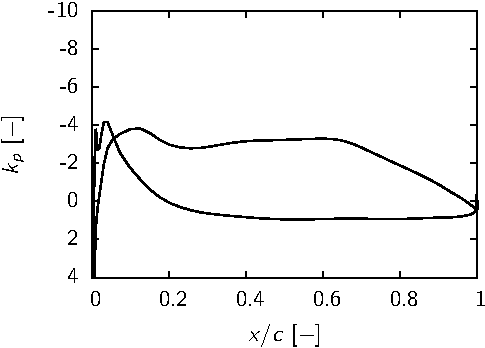
\includegraphics[width=0.28\textwidth]{DREAM_HS_KP_50_FRONT_PPT.pdf}
   & 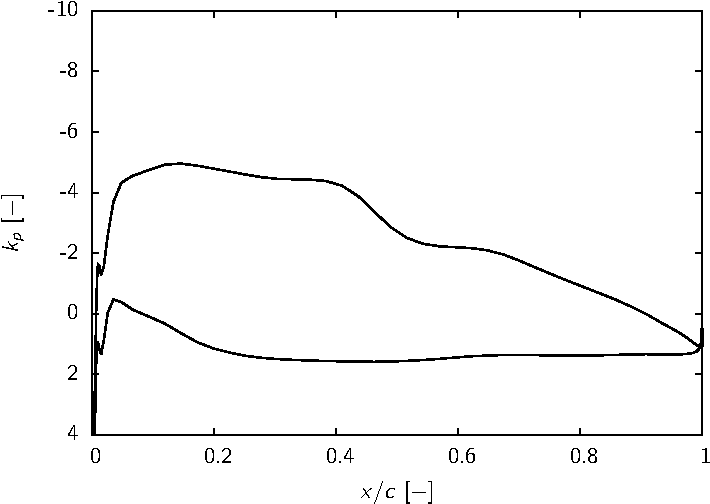
\includegraphics[width=0.28\textwidth]{DREAM_HS_KP_50_REAR_PPT.pdf}
   & 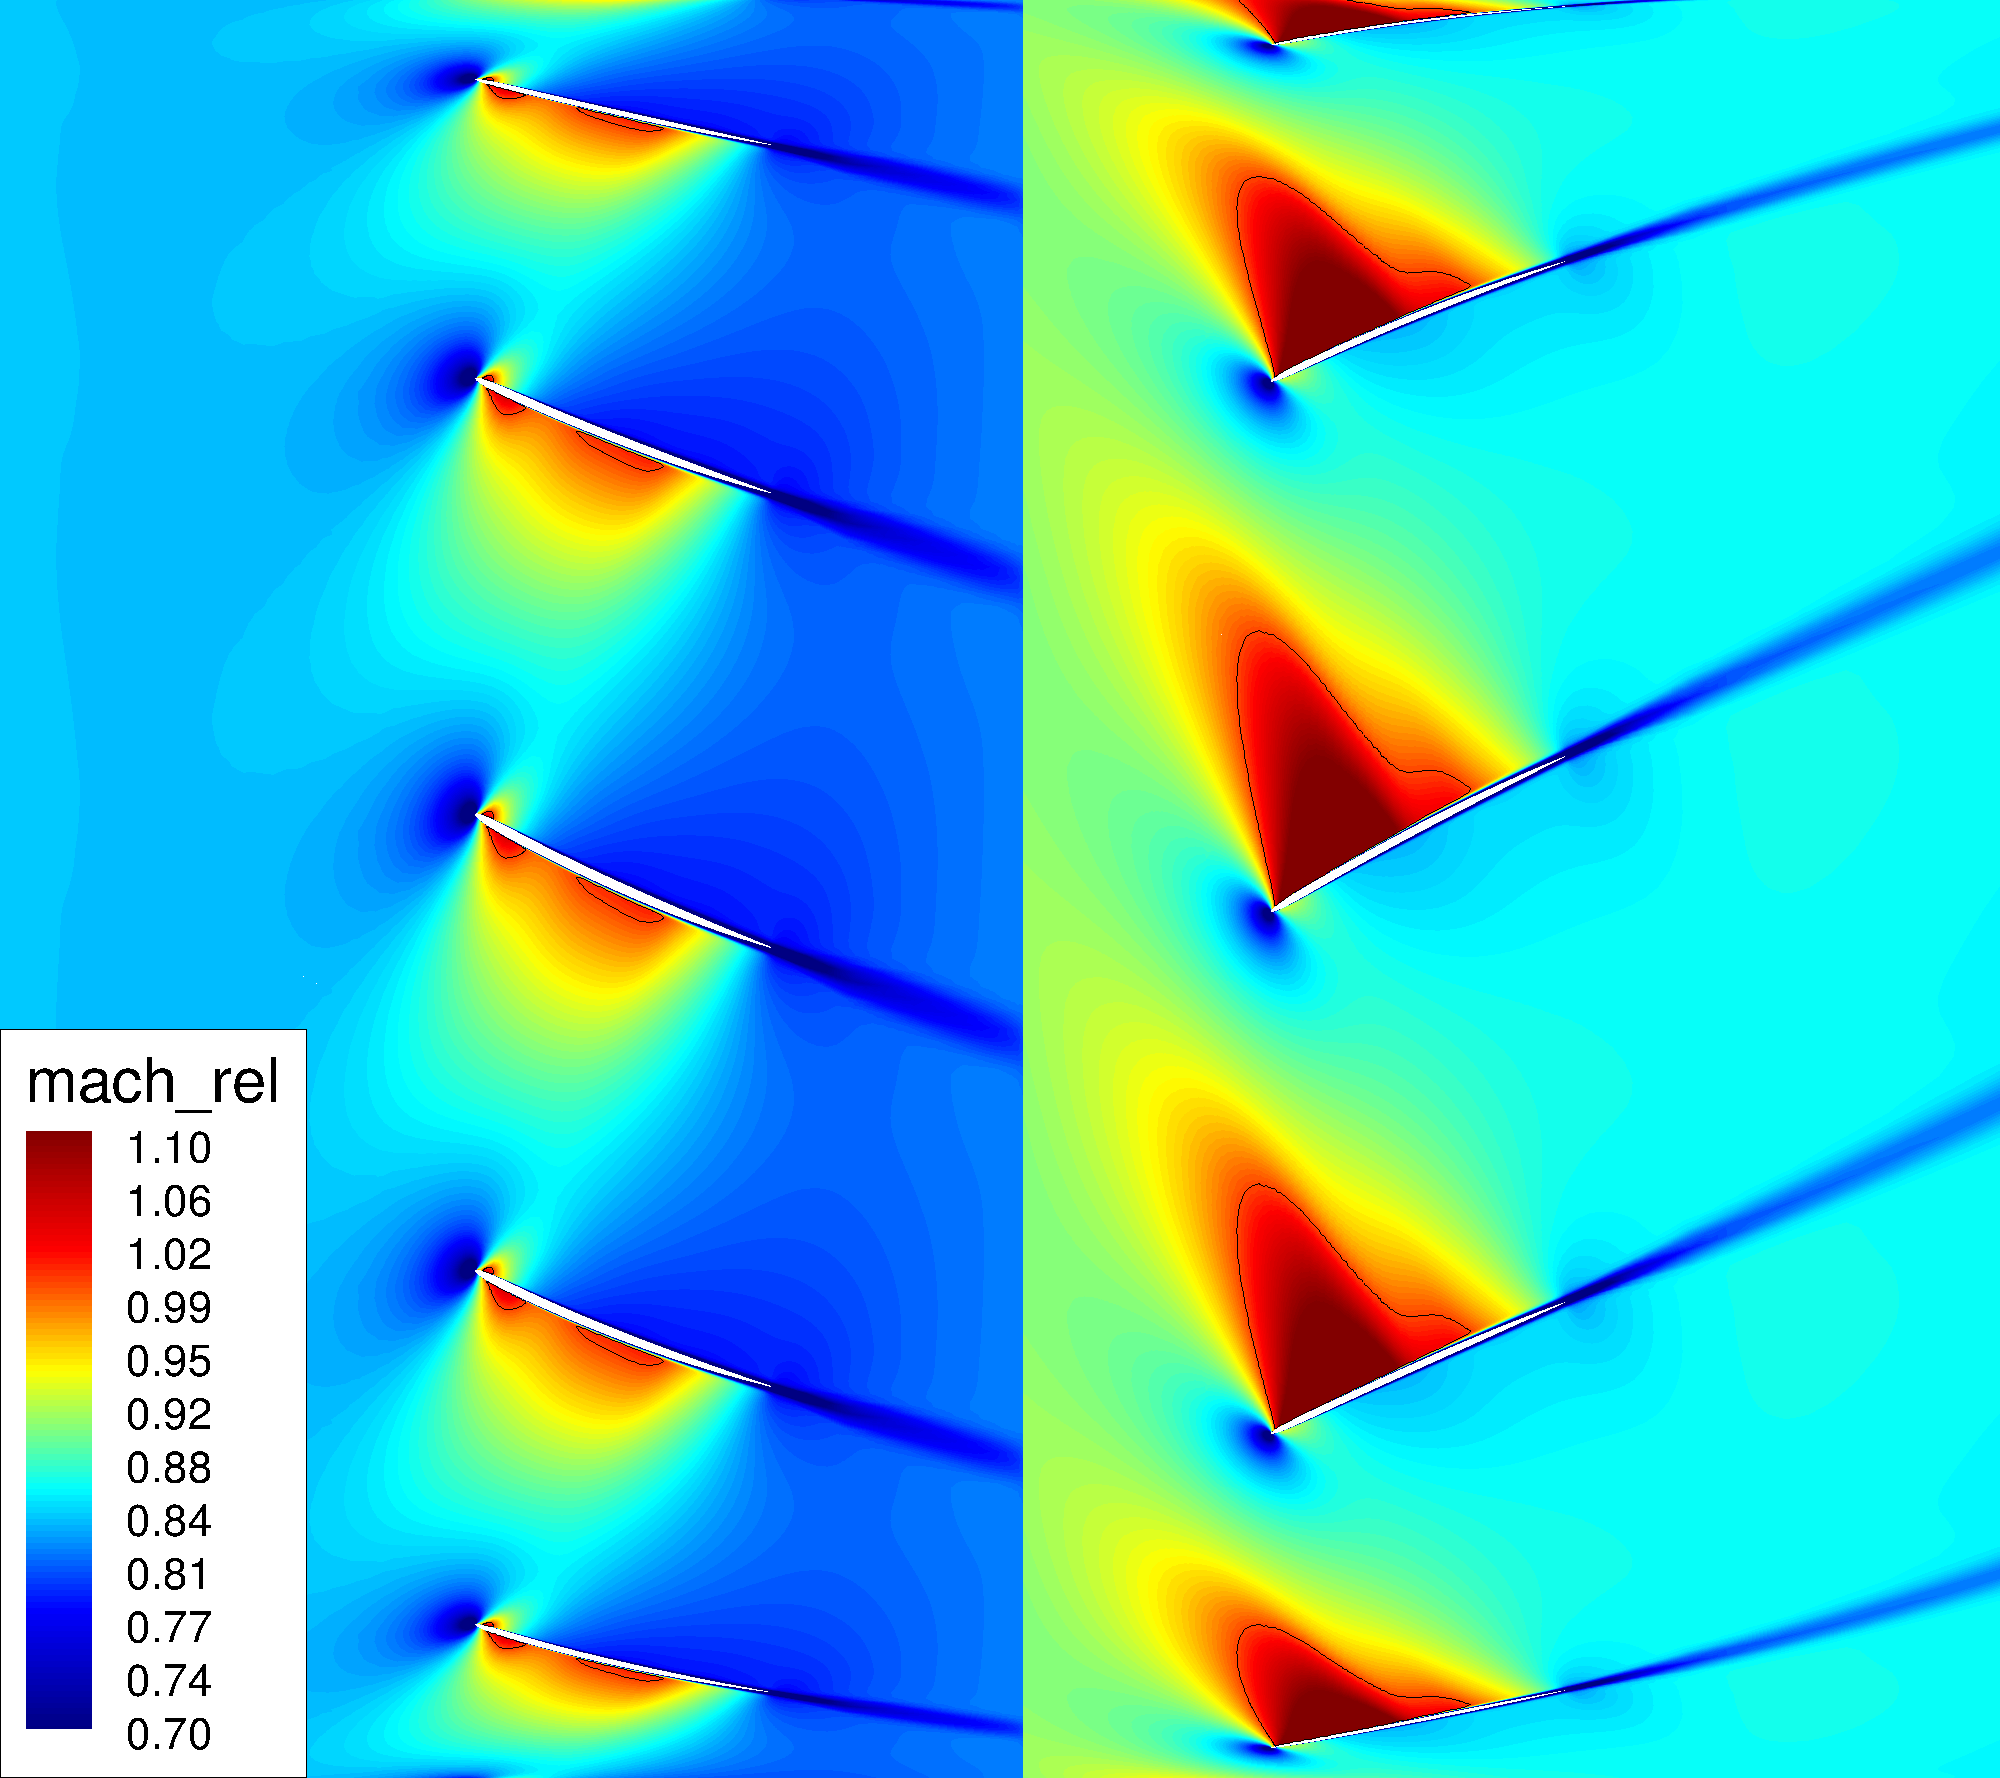
\includegraphics[width=0.28\textwidth]{DREAM_HS_RANS_roe2_sa_slice_r_50_mach_rel.png}\\
   \rotatebox{90}{\qquad\qquad 75~\%} 
   & 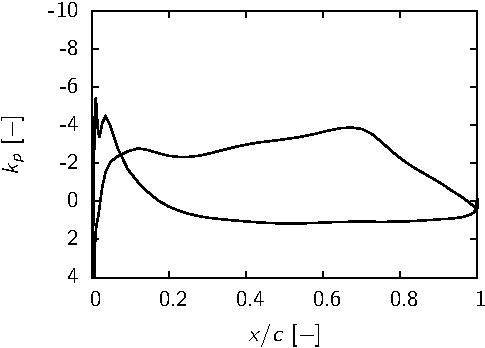
\includegraphics[width=0.28\textwidth]{DREAM_HS_KP_75_FRONT_PPT.pdf}
   & 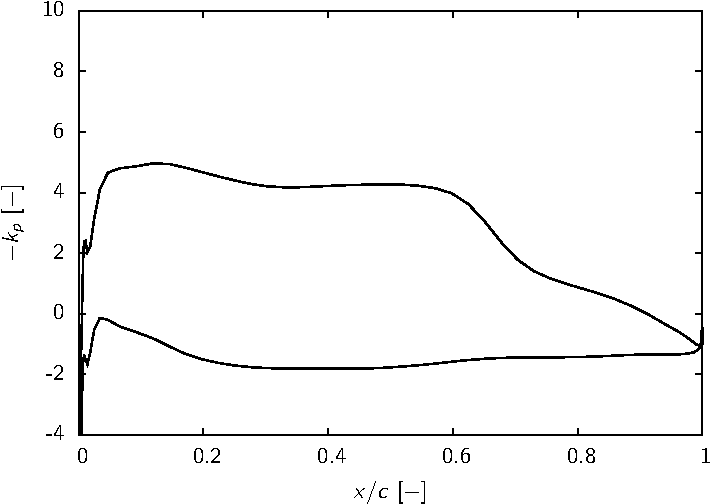
\includegraphics[width=0.28\textwidth]{DREAM_HS_KP_75_REAR_PPT.pdf}
   & 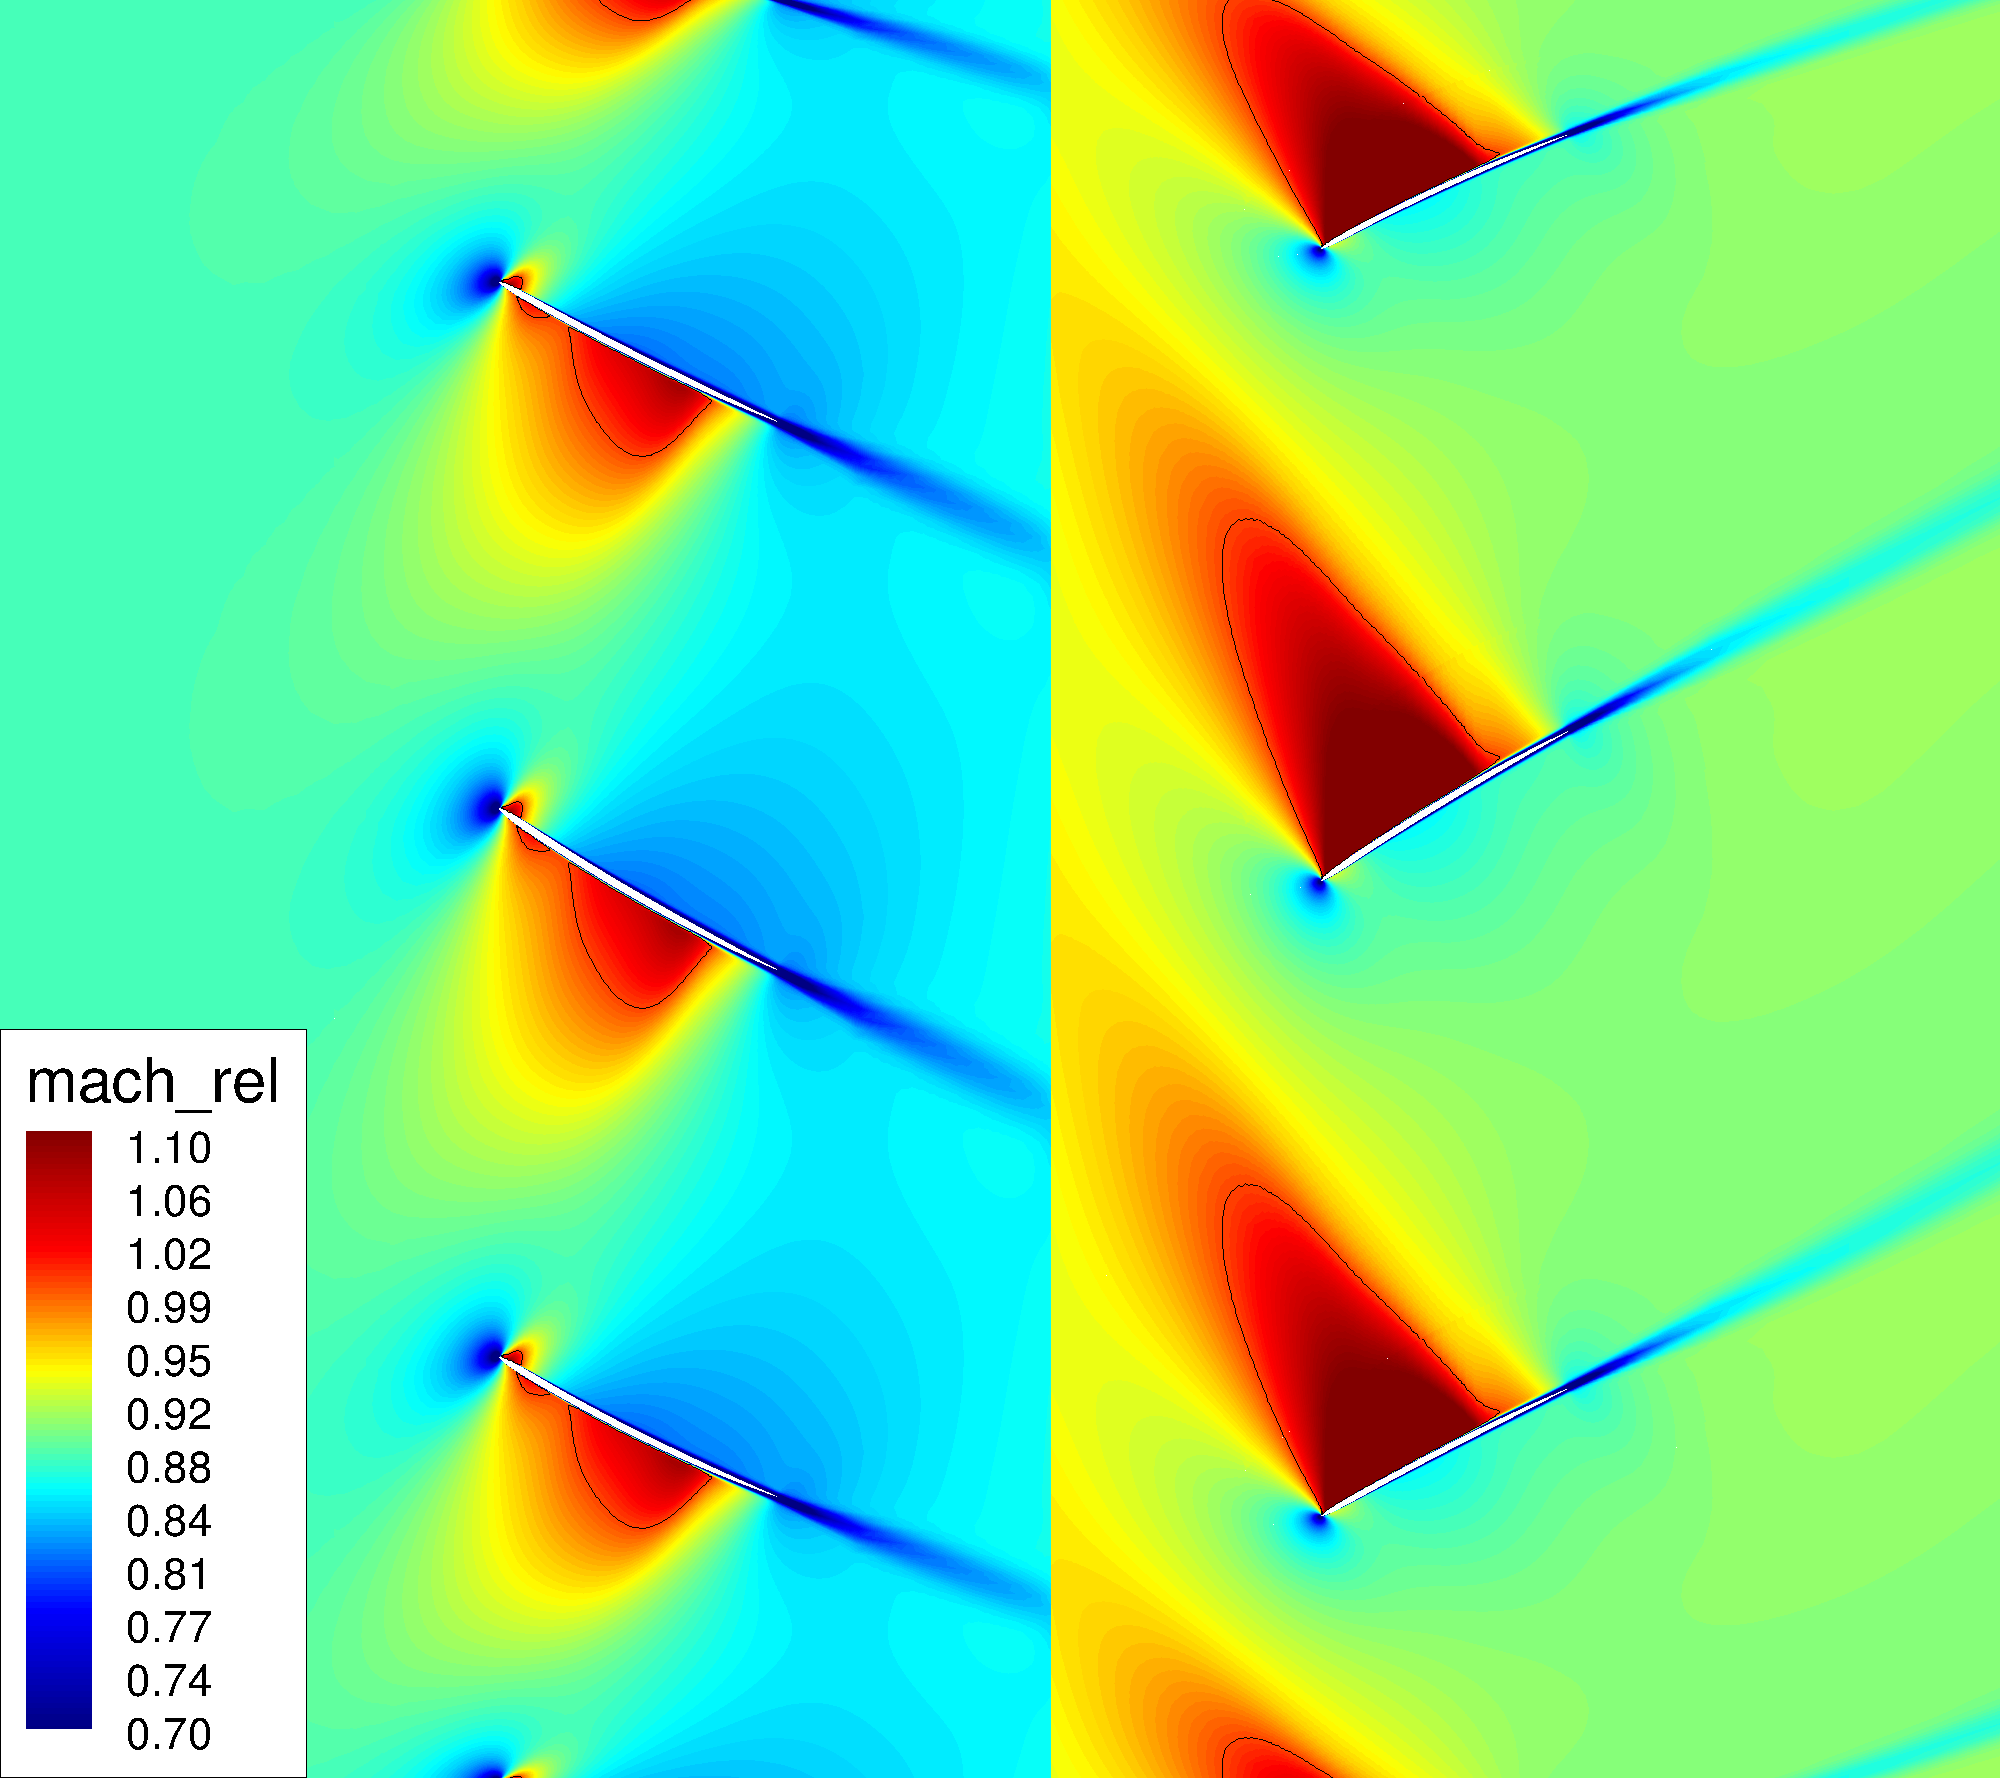
\includegraphics[width=0.28\textwidth]{DREAM_HS_RANS_roe2_sa_slice_r_75_mach_rel.png}\\
   \rotatebox{90}{\qquad\qquad 90~\%} 
   & 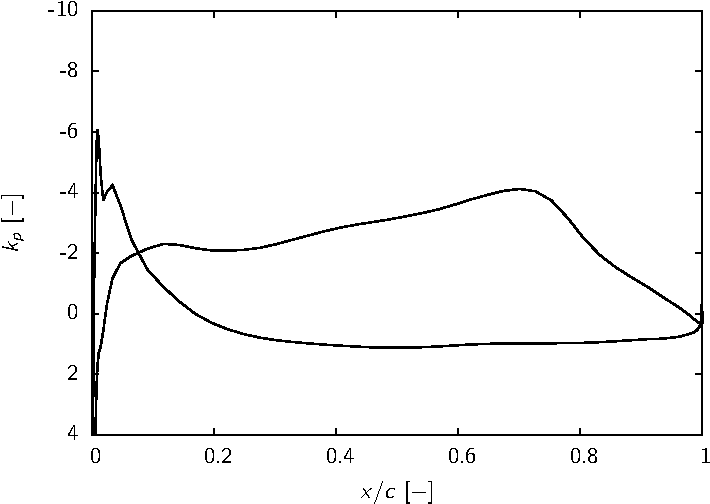
\includegraphics[width=0.28\textwidth]{DREAM_HS_KP_90_FRONT_PPT.pdf}
   & 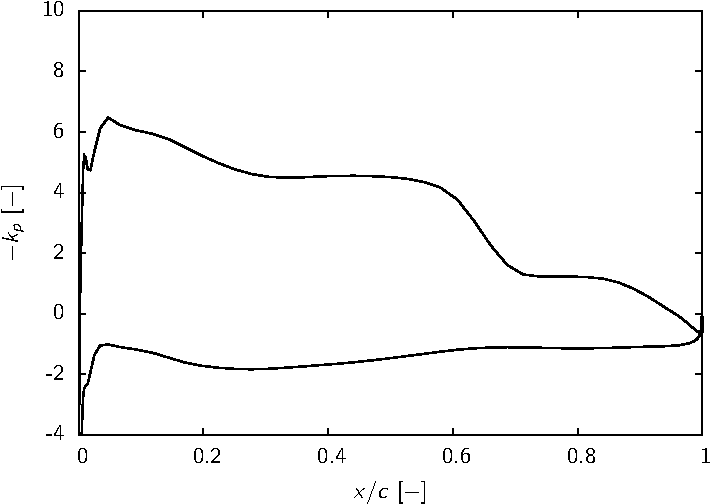
\includegraphics[width=0.28\textwidth]{DREAM_HS_KP_90_REAR_PPT.pdf}
   & 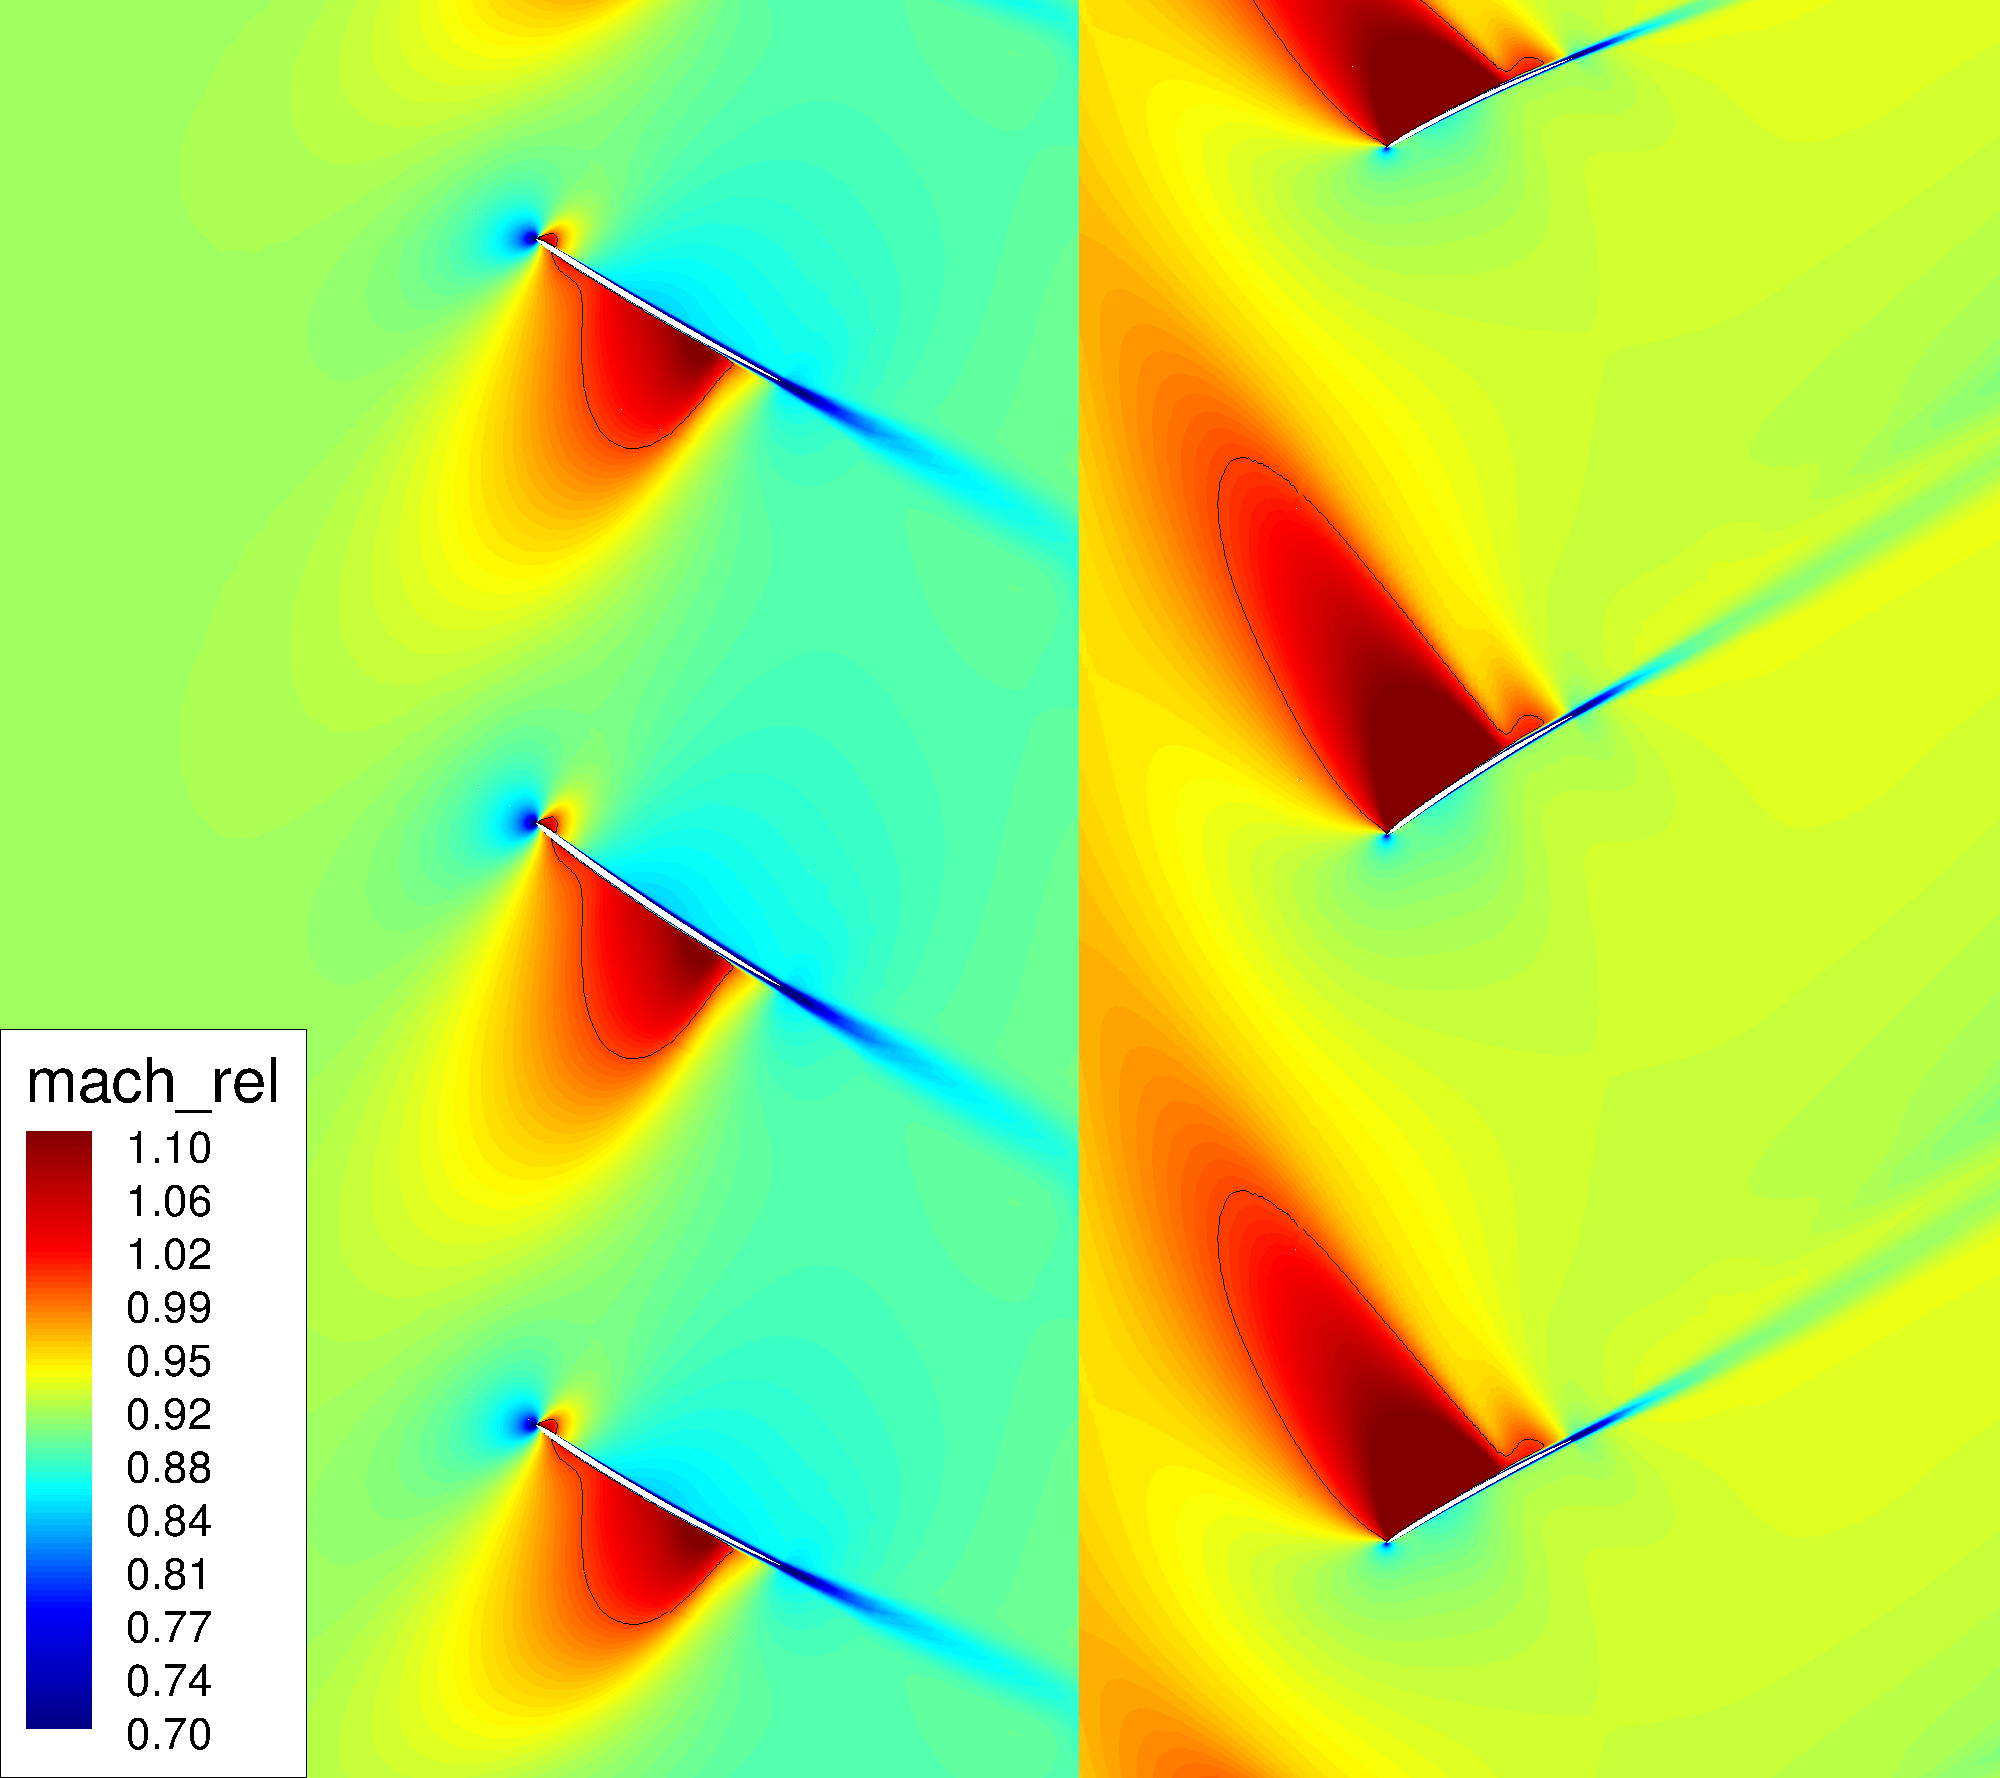
\includegraphics[width=0.28\textwidth]{DREAM_HS_RANS_roe2_sa_slice_r_90_mach_rel.png}\\
   \rotatebox{90}{\qquad\qquad 95~\%} 
   & 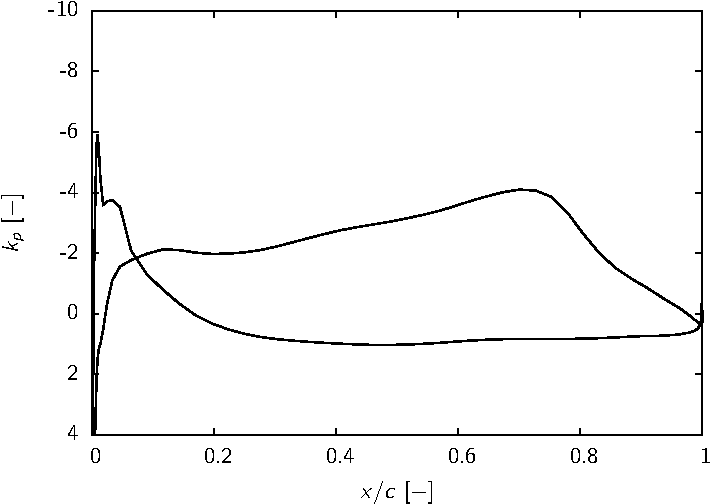
\includegraphics[width=0.28\textwidth]{DREAM_HS_KP_95_FRONT_PPT.pdf}
   & 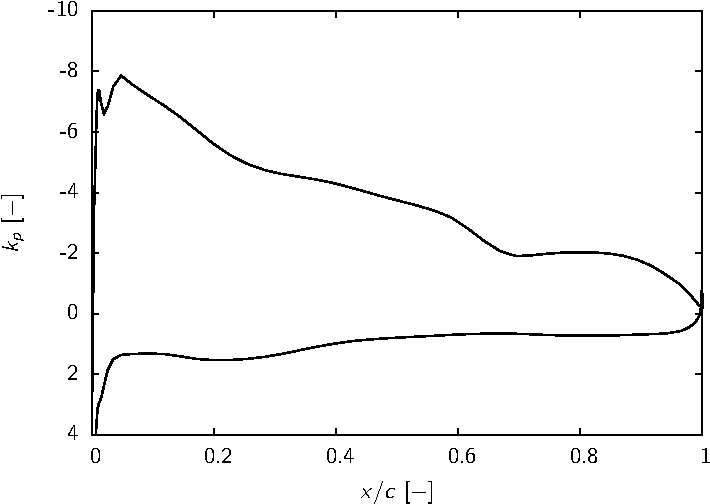
\includegraphics[width=0.28\textwidth]{DREAM_HS_KP_95_REAR_PPT.pdf}
   & 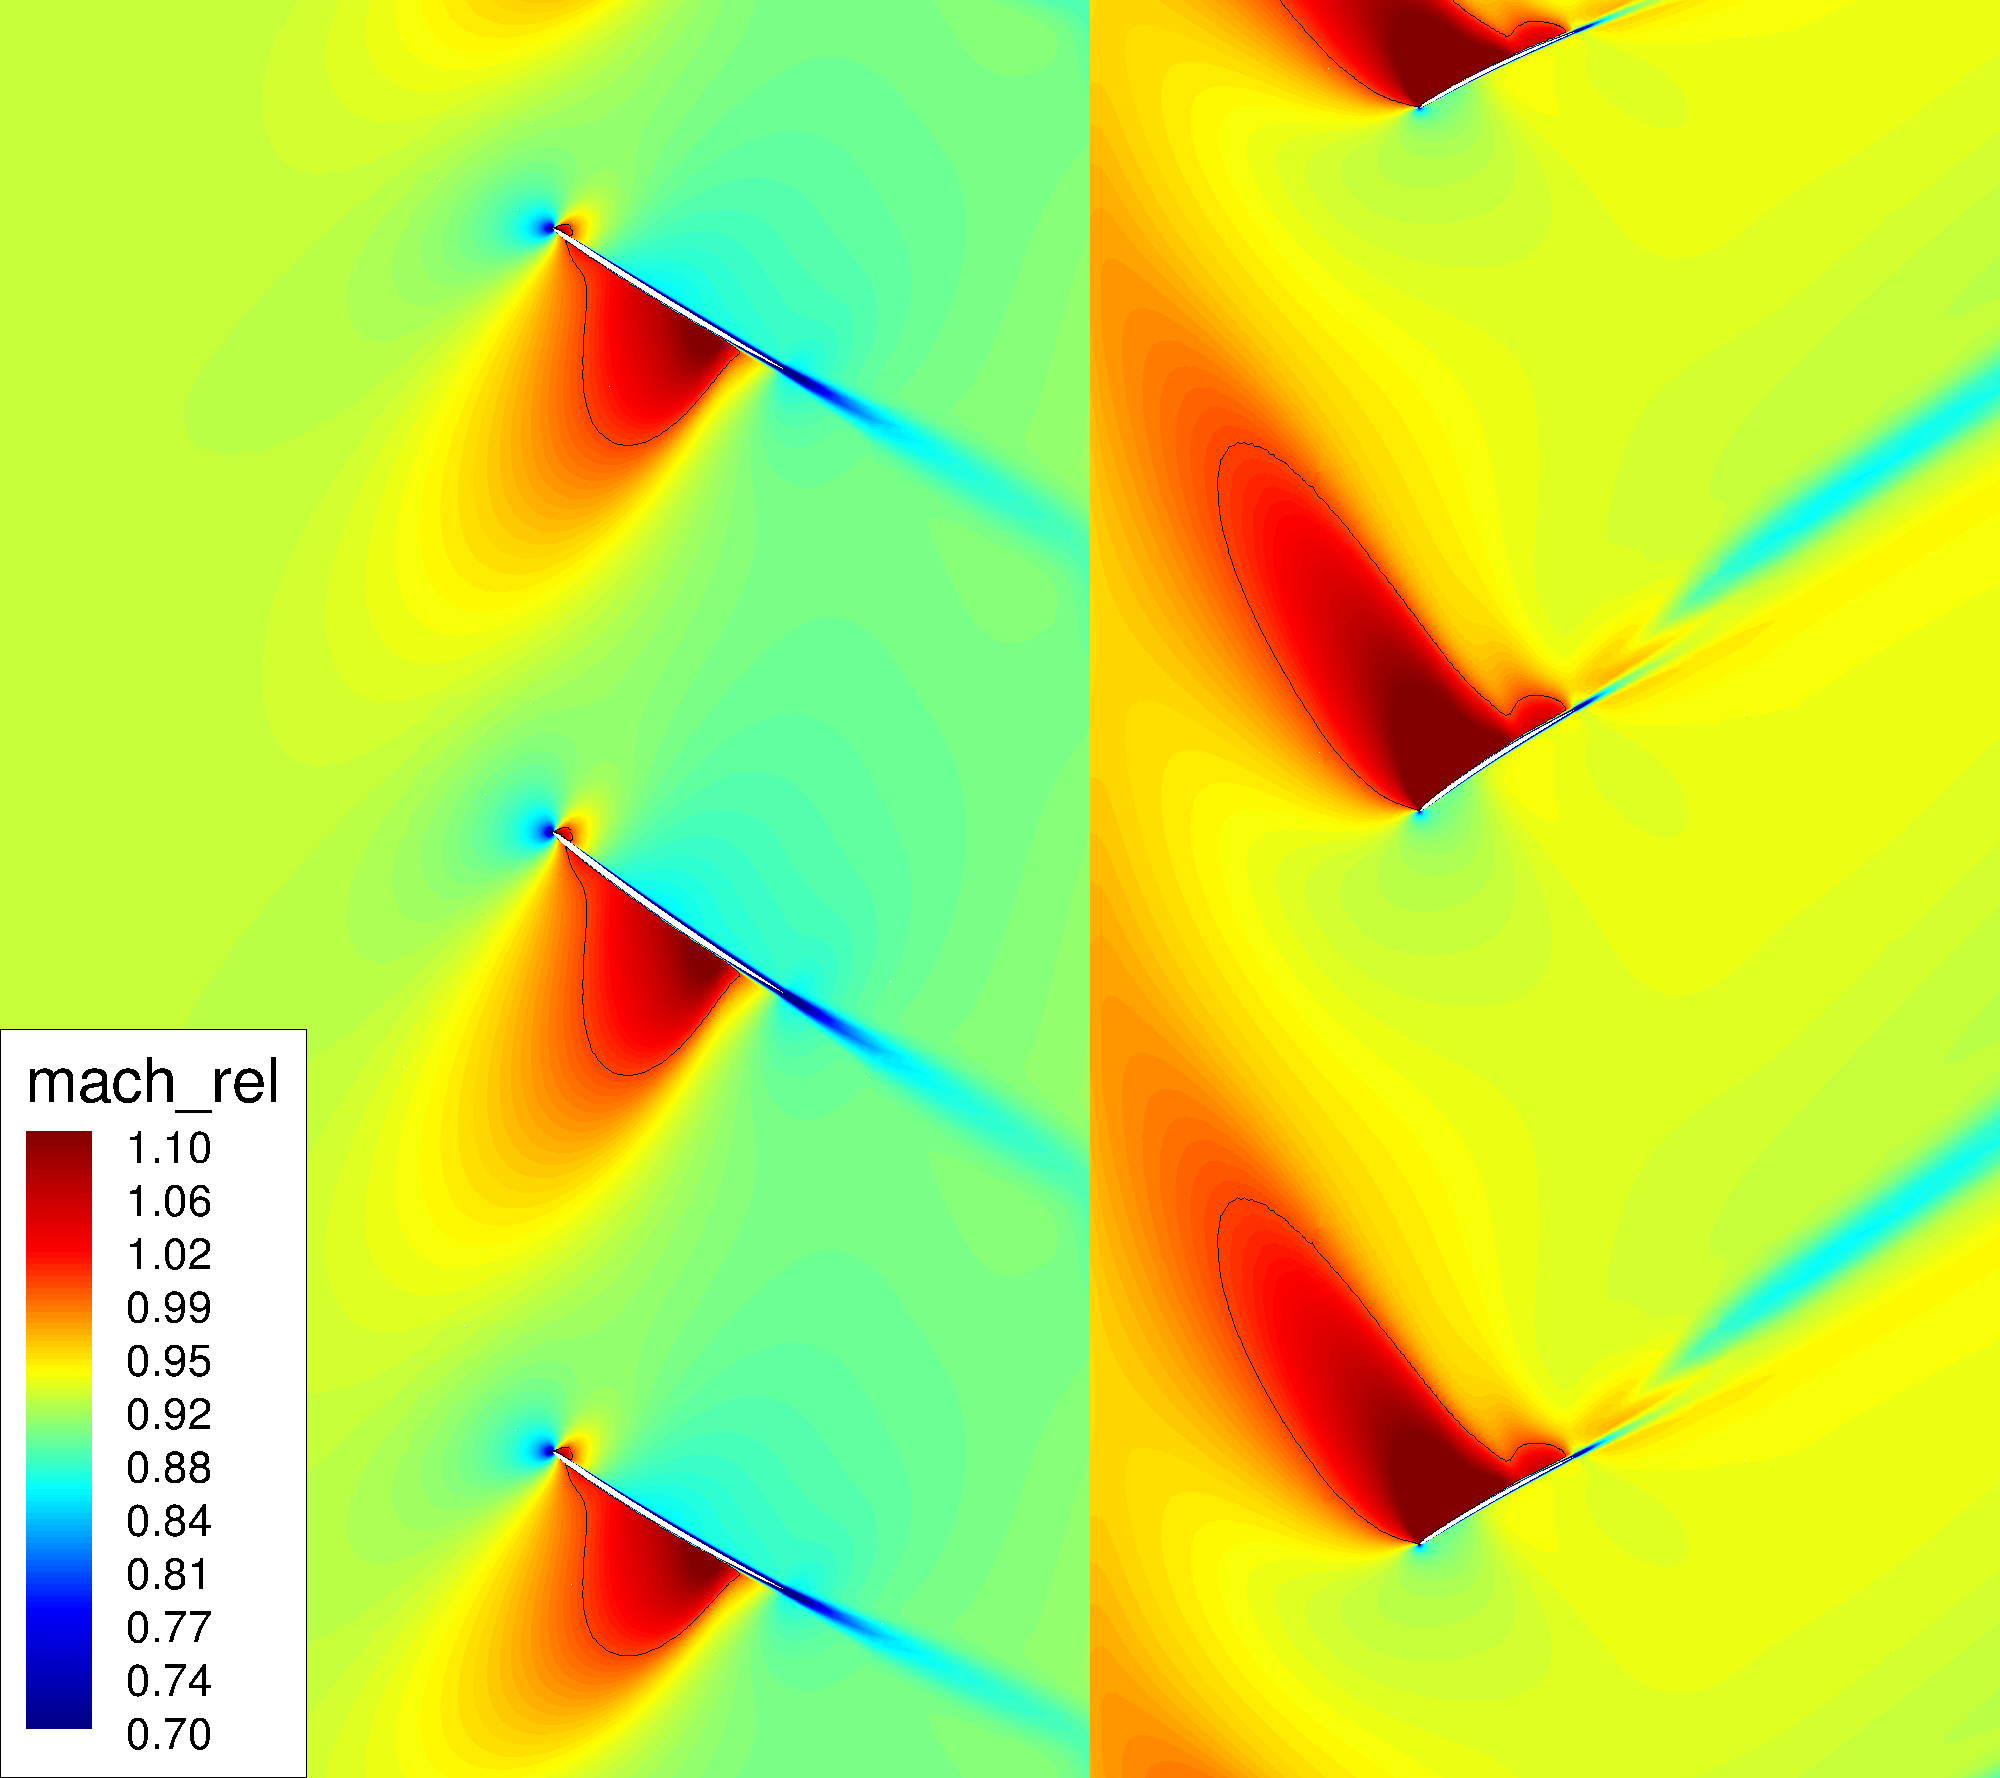
\includegraphics[width=0.28\textwidth]{DREAM_HS_RANS_roe2_sa_slice_r_95_mach_rel.png}  
 \end{tabular}
 \caption{High-speed isolated configuration: pressure coefficient and relative Mach
 number contours at different radial position.}
 \label{fig:dream_HS_mach_kp}
\end{figure}

\begin{figure}[htp]
  \centering
  \subfigure[$P3$]{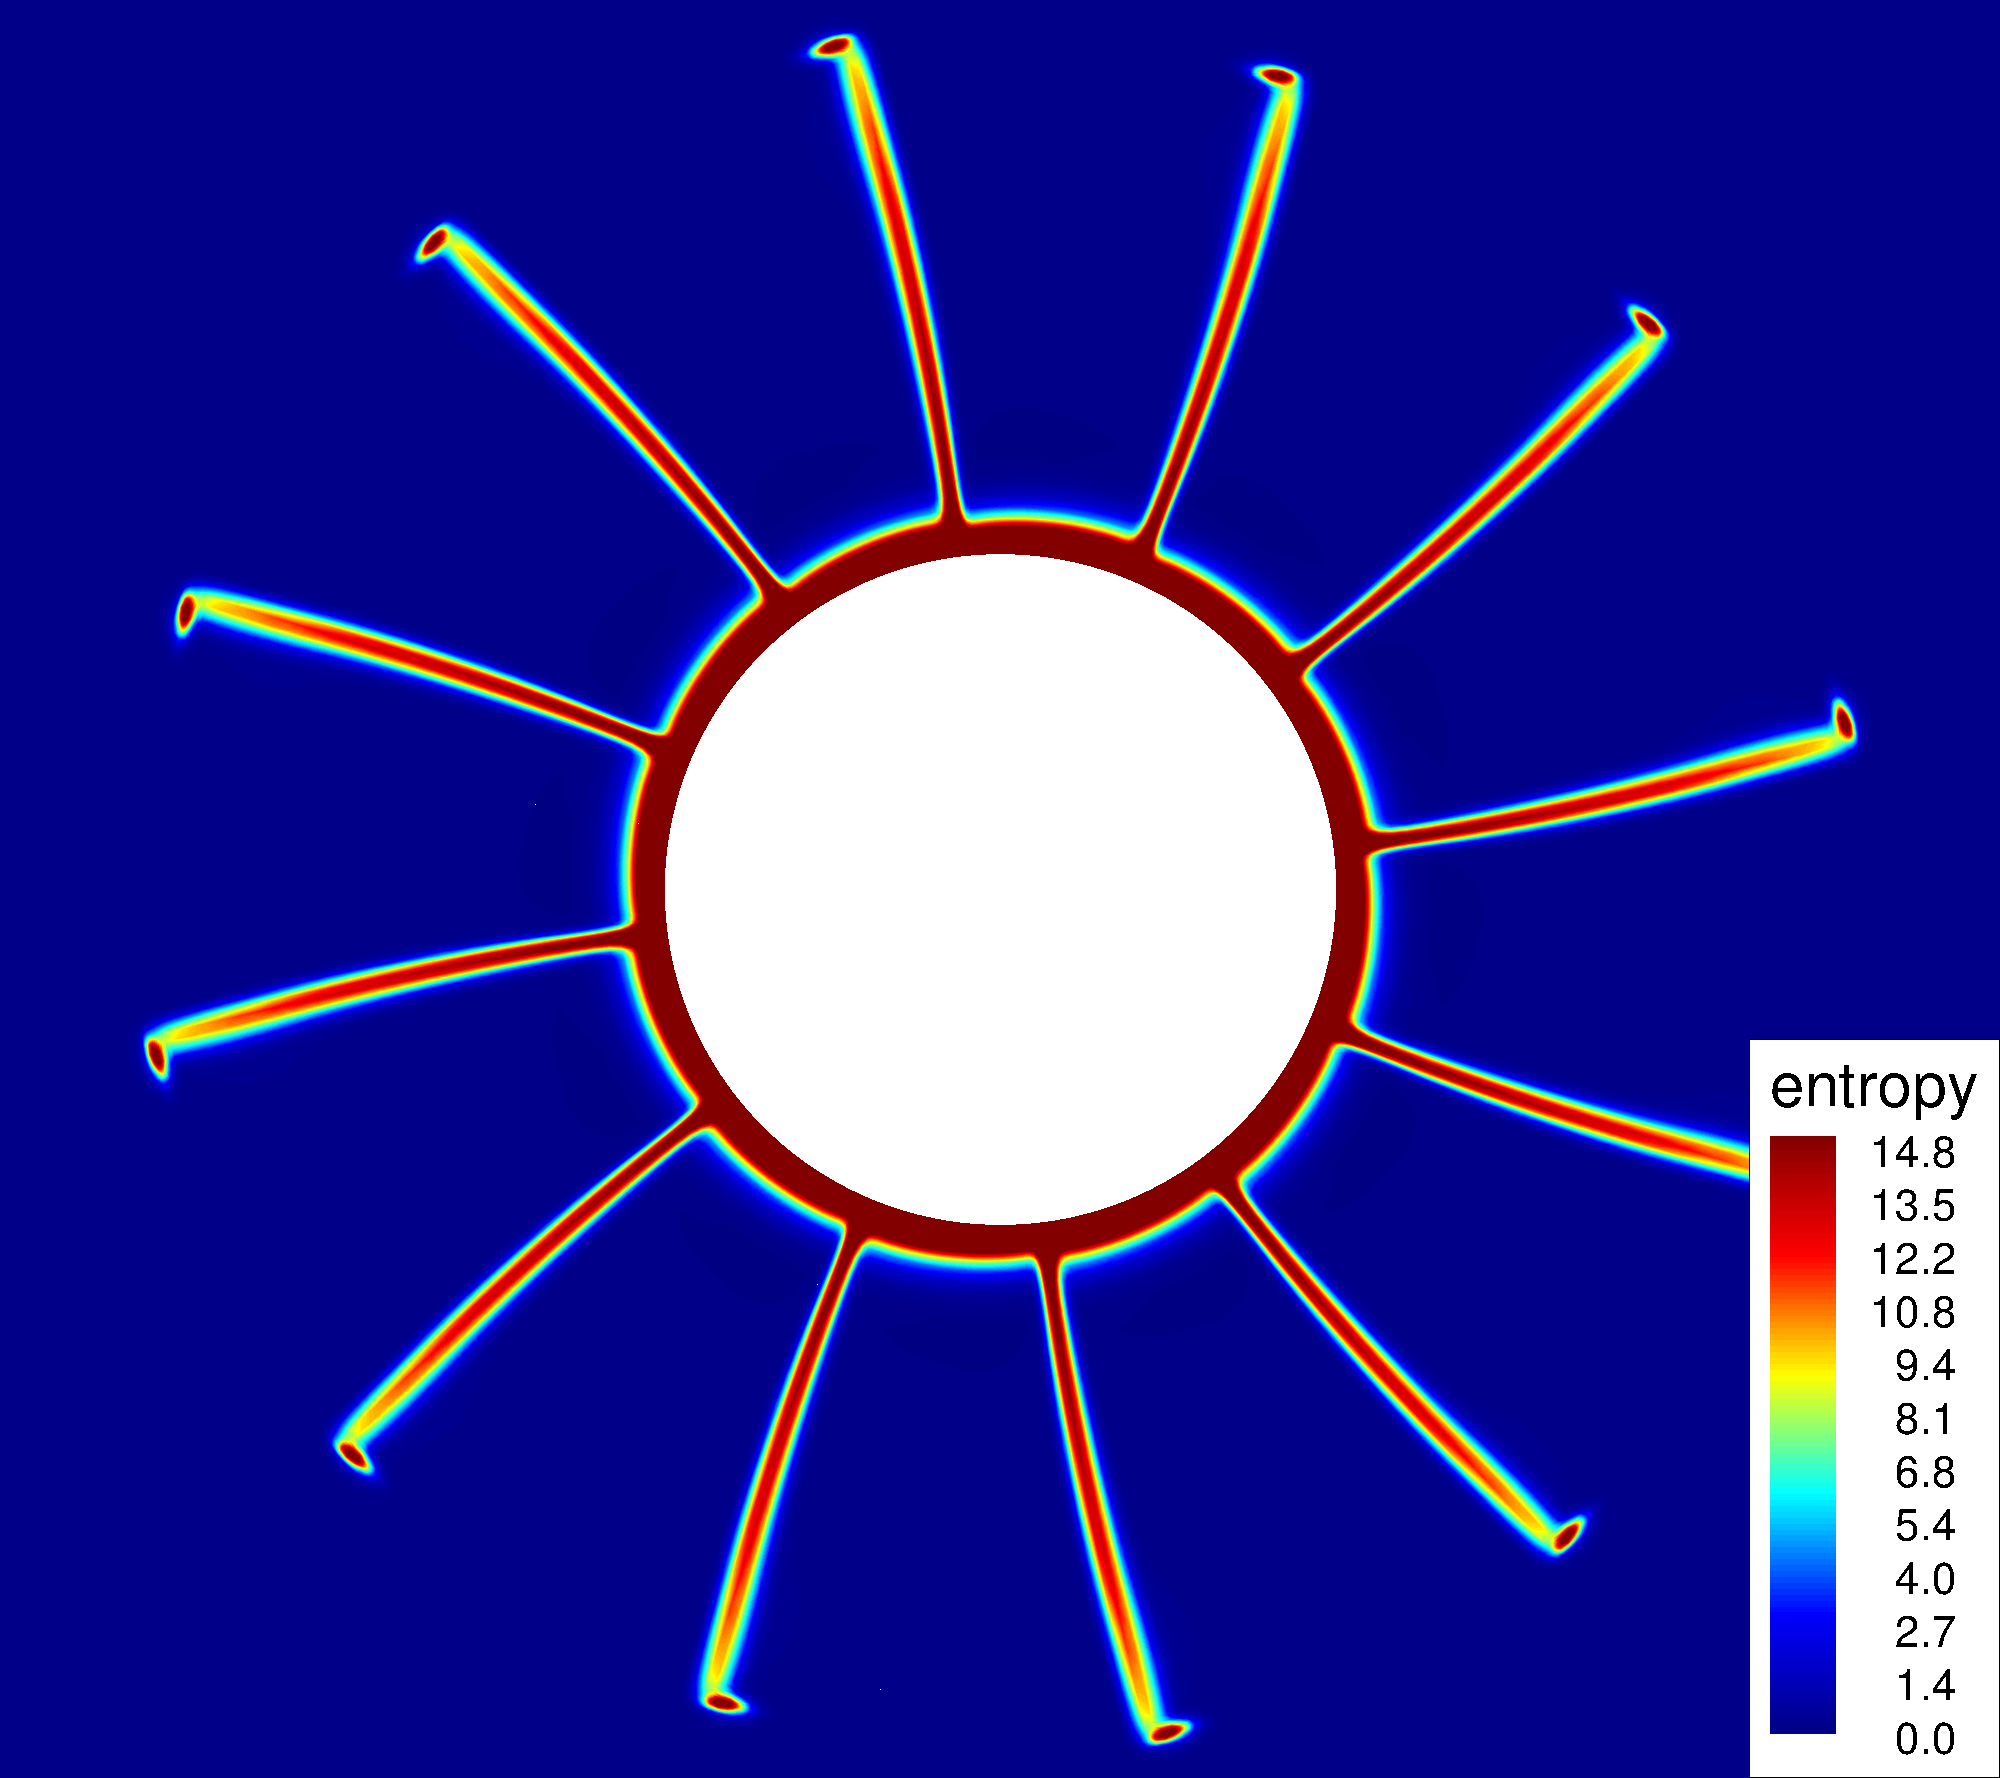
\includegraphics[width=.35\textwidth]{DREAM_HS_RANS_roe2_sa_slice_x_front_1_entropy.png}}
  \subfigure[$P4$]{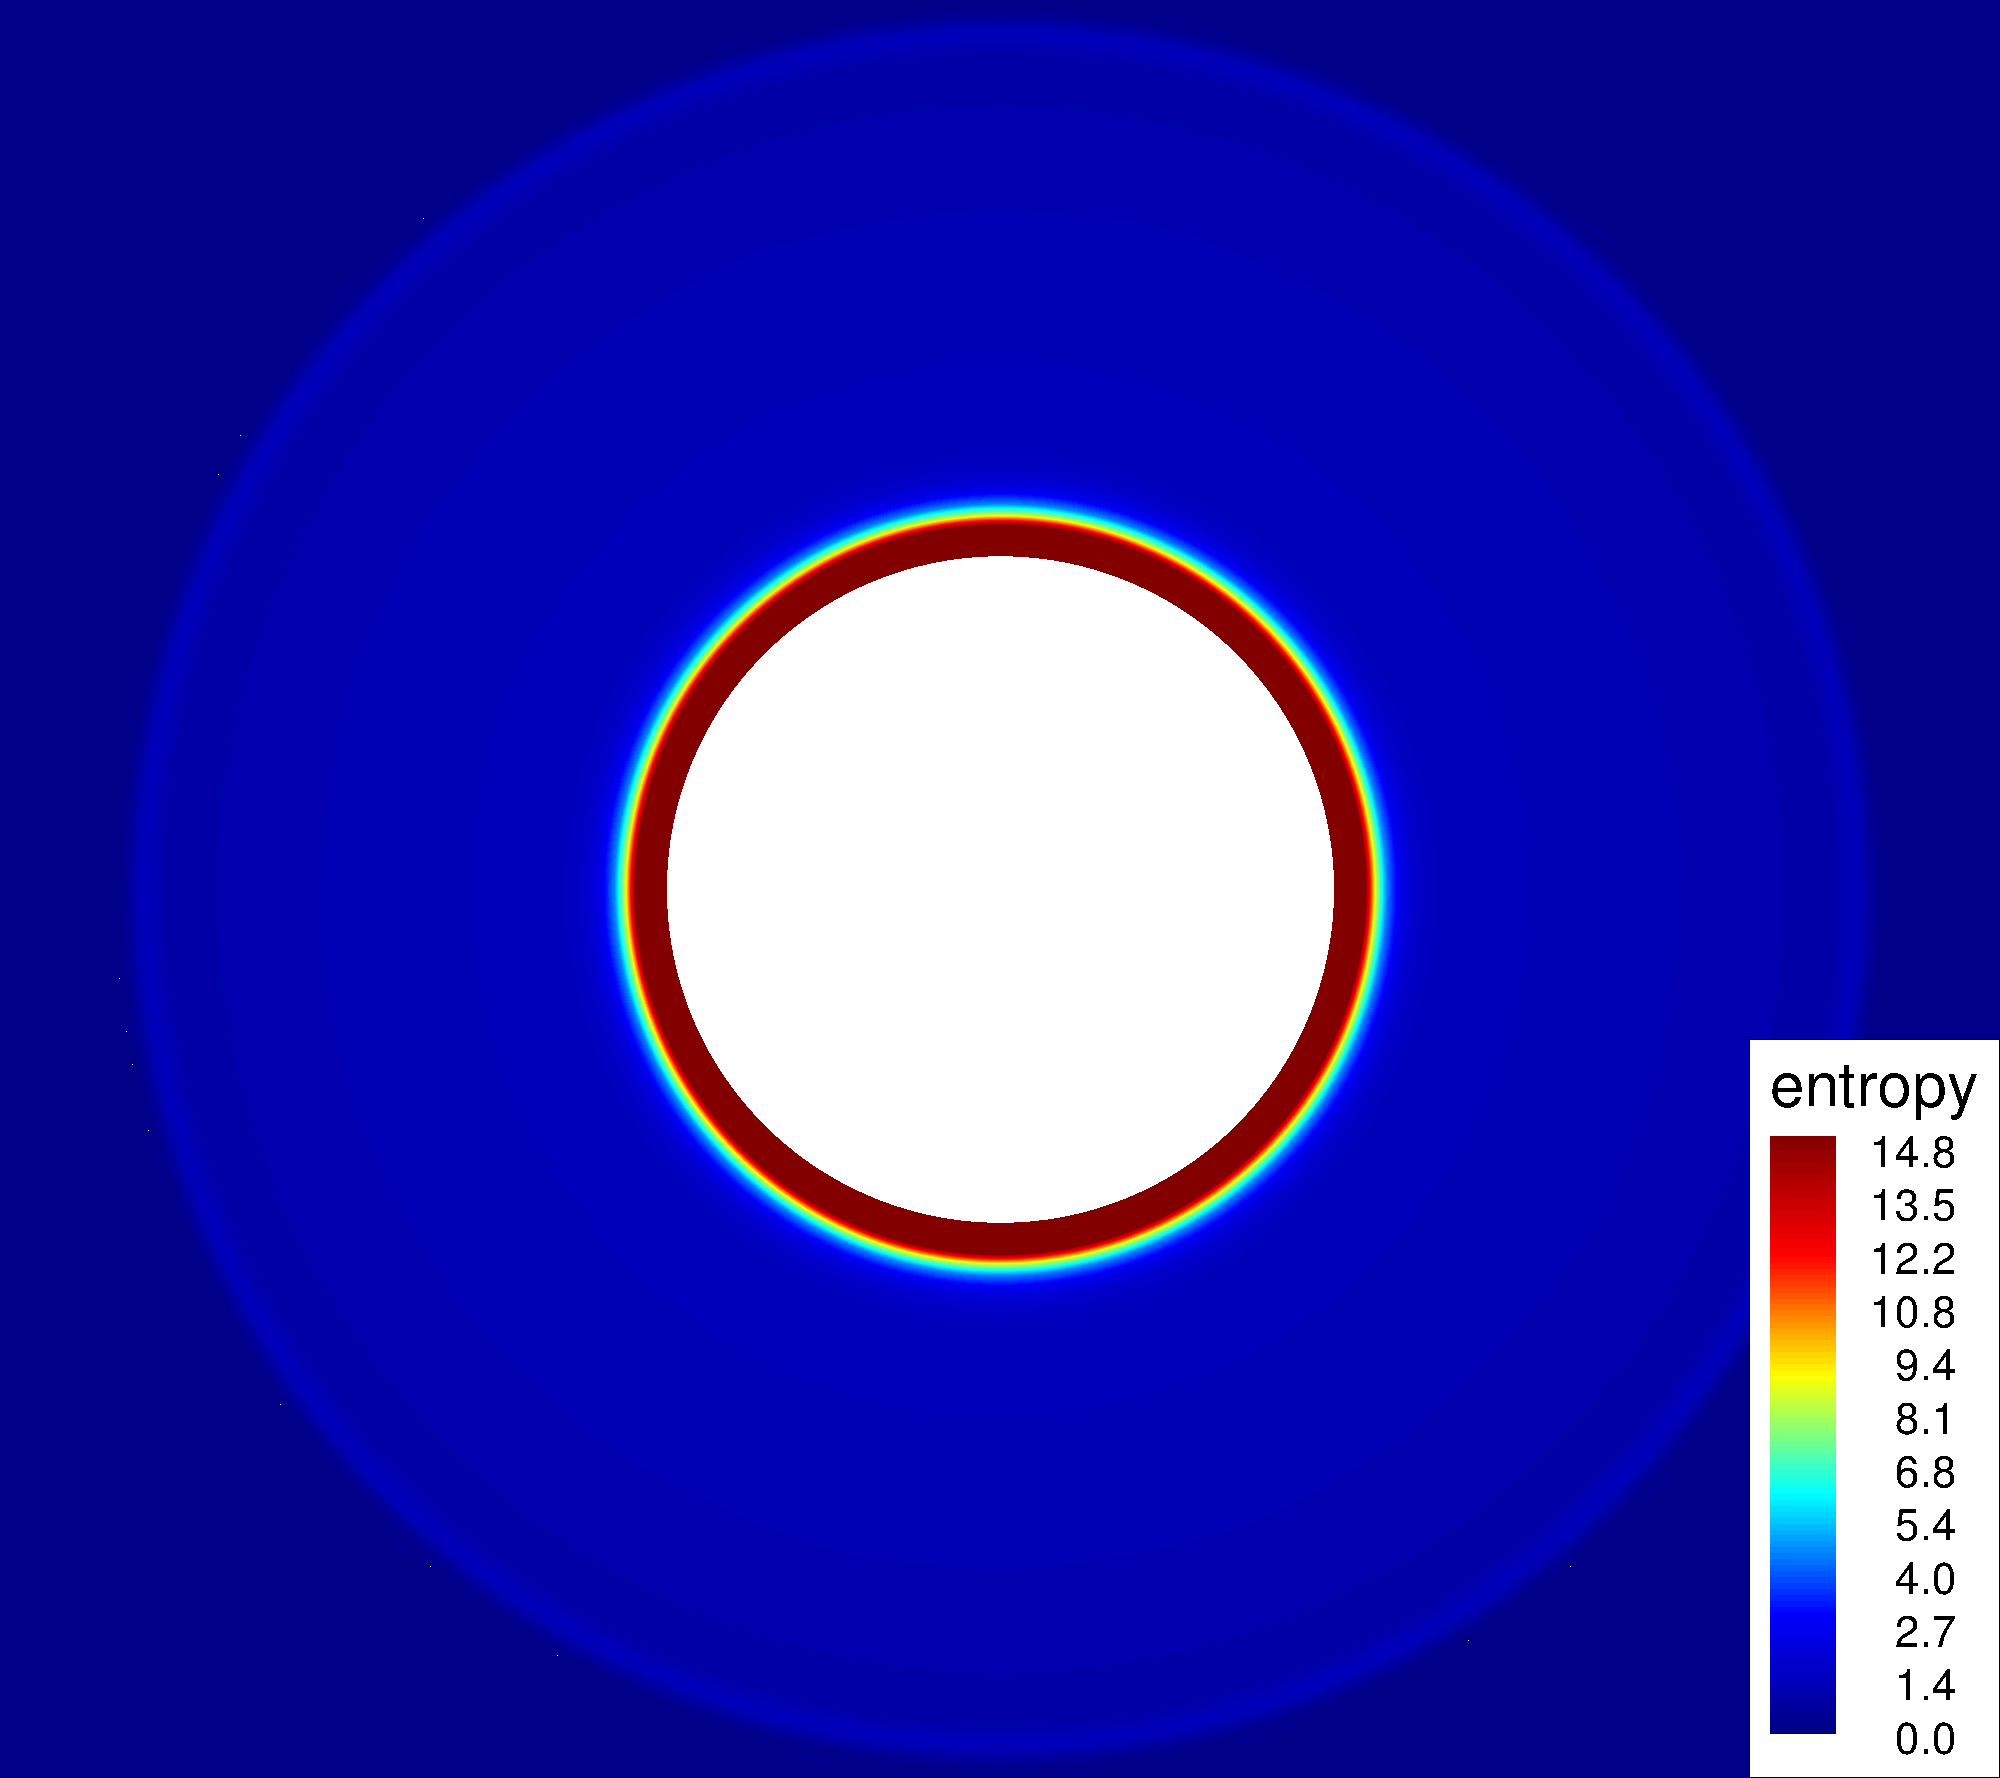
\includegraphics[width=.35\textwidth]{DREAM_HS_RANS_roe2_sa_slice_x_rear_0_entropy.png}}
  \subfigure[$P5$]{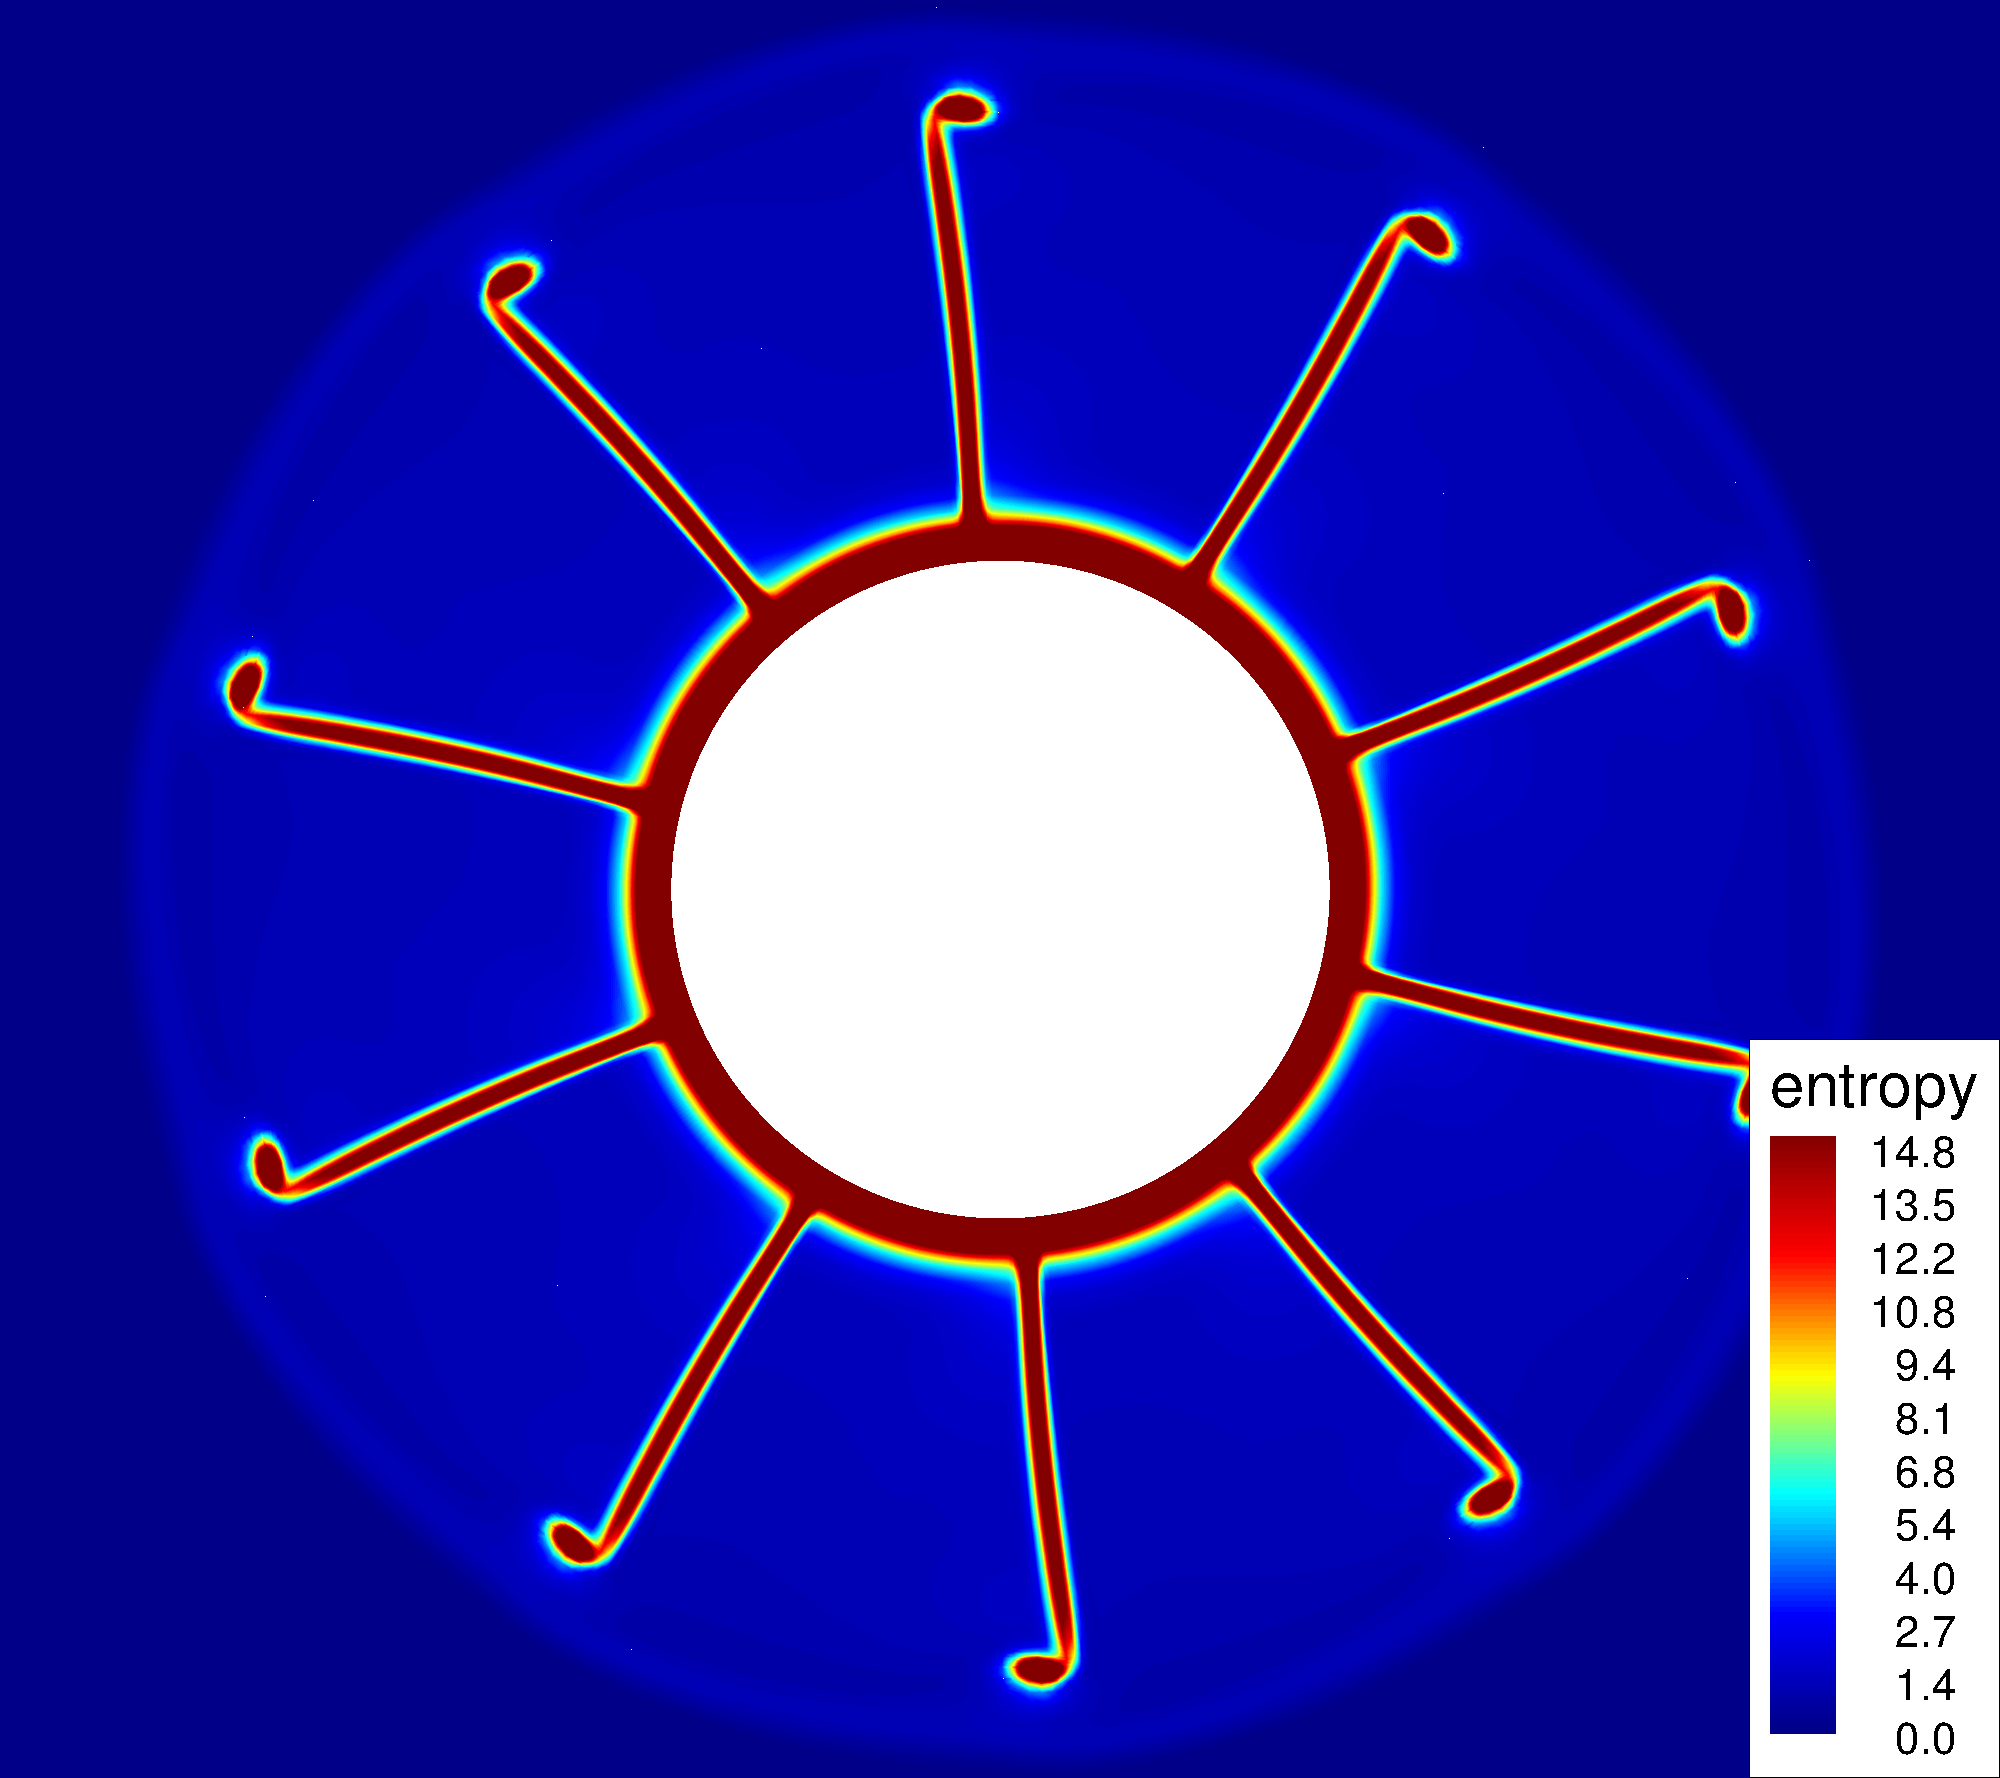
\includegraphics[width=.35\textwidth]{DREAM_HS_RANS_roe2_sa_slice_x_rear_1_entropy.png}}
  \subfigure[$P6$]{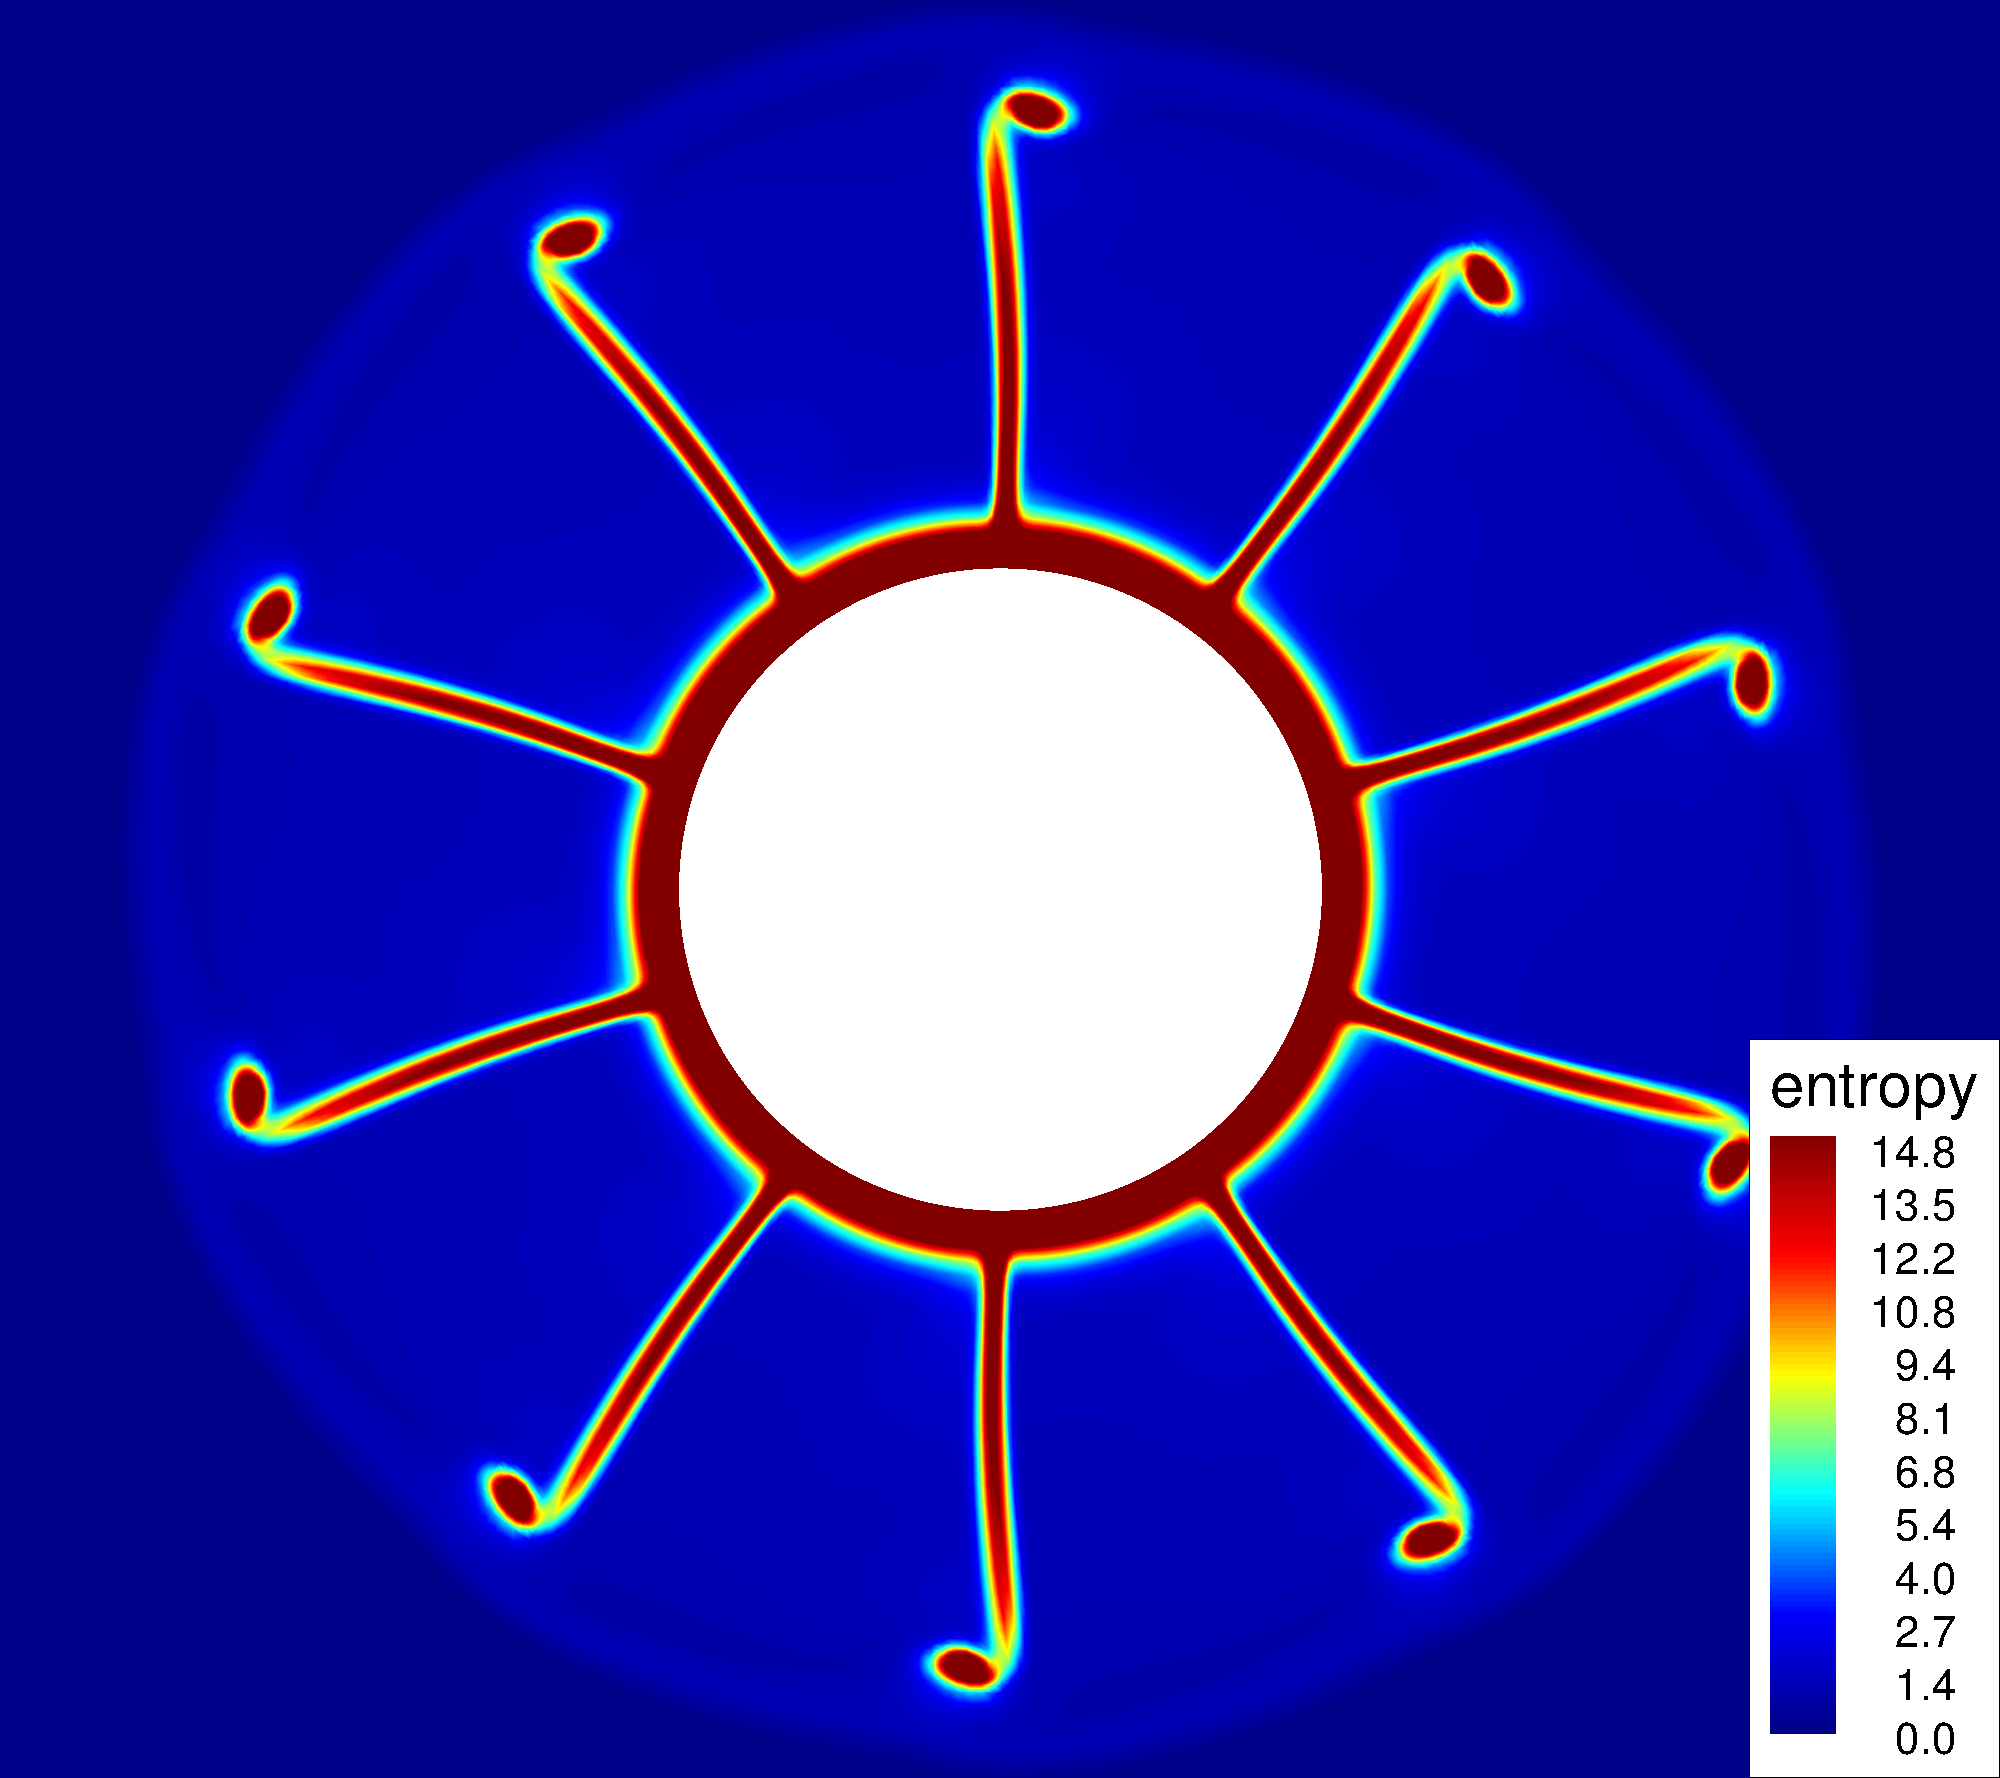
\includegraphics[width=.35\textwidth]{DREAM_HS_RANS_roe2_sa_slice_x_rear_2_entropy.png}}
  \caption{High-speed isolated configuration: axial cut of entropy.}
   \label{fig:dream_HS_steady_entropy}
\end{figure}

\section{\emph{a priori} estimate of the required number of harmonics}
\label{sec:dream_hs_spectral_convergence}
%!TEX root = ../../../adrien_gomar_phd.tex


\begin{figure}[htp]
  \centering
  \includegraphics*[width=0.5\textwidth]{DREAM_HS_RANS_ROE2_SPECTRUM_PPT.pdf}
  \caption{High-speed isolated configuration: prediction of the number
  of harmonics needed to simulate the configuration.}
  \label{fig:DREAM_HS_RANS_ROE2_SPECTRUM_PPT}
\end{figure}




\section{Unsteady rigid results}
\label{sec:dream_hs_rigid_results}
%!TEX root = ../../../adrien_gomar_phd.tex

\subsection{Similarity coefficients}
\label{sub:dream_hs_hb_sim_coeff}


The level of unsteadiness perceived by both rotors is reported
in Fig.~\ref{fig:dream_hs_hb_unst_coeff} for the thrust coefficient.
\begin{figure}[htp]
  \centering
  \subfigure[front rotor]{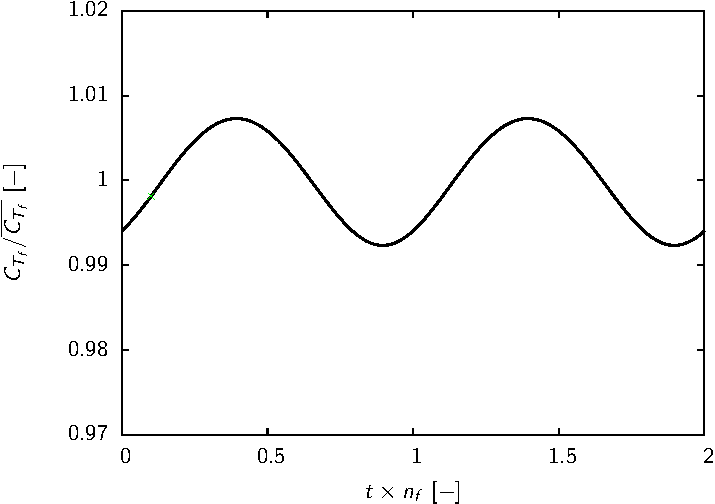
\includegraphics[width=.35\textwidth]{DREAM_HS_TSM_FORCES_INST_FRONT_PPT.pdf}}
  \subfigure[rear rotor]{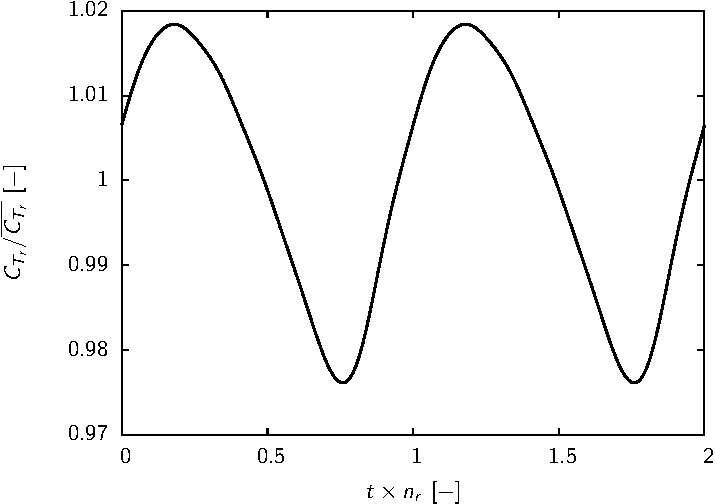
\includegraphics[width=.35\textwidth]{DREAM_HS_TSM_FORCES_INST_REAR_PPT.pdf}}
  \caption{High-speed isolated configuration: unsteadiness seen by the rotors.}
  \label{fig:dream_hs_hb_unst_coeff}
\end{figure}
The envelop of the unsteadiness is $\pm 1\%$ on the front rotor
and $\pm 2\%$ on the rear rotor. This has to be compared to 
the $\pm 3 \permil$ observed for the low-speed configuration.
The amplitude of unsteadiness is double on the rear rotor
meaning that the wake effects are much stronger than the
potential ones when considering the high-speed inflow condition.
The analysis of the shape of the unsteady thrust coefficient
reveals that it is close to a sine shape function for the front
rotor. It tends toward a Gaussian shape function for the rear rotor.

\subsection{Two-dimensional results: harmonic blade response}
\label{sub:dream_hs_hb_blade_response}

To further analyze the unsteadinesses perceived by both rotors,
a discrete Fourier transform of the first harmonic of the static pressure
of the opposite blade passing frequency is shown in 
Fig.~\ref{fig:dream_hs_hb_blade_response}. Note that the
scale is different for the front and the rear rotors.
\begin{figure}[htp]
 \ra{1.3} \centering
 \begin{tabular}{cccc}
    \multicolumn{2}{c}{\includegraphics[width=0.3\textwidth]{dream_HS_blade_resp_scale_H01_front.pdf}} &
    \multicolumn{2}{c}{\includegraphics[width=0.3\textwidth]{dream_HS_blade_resp_scale_H01_rear.pdf}} \\
    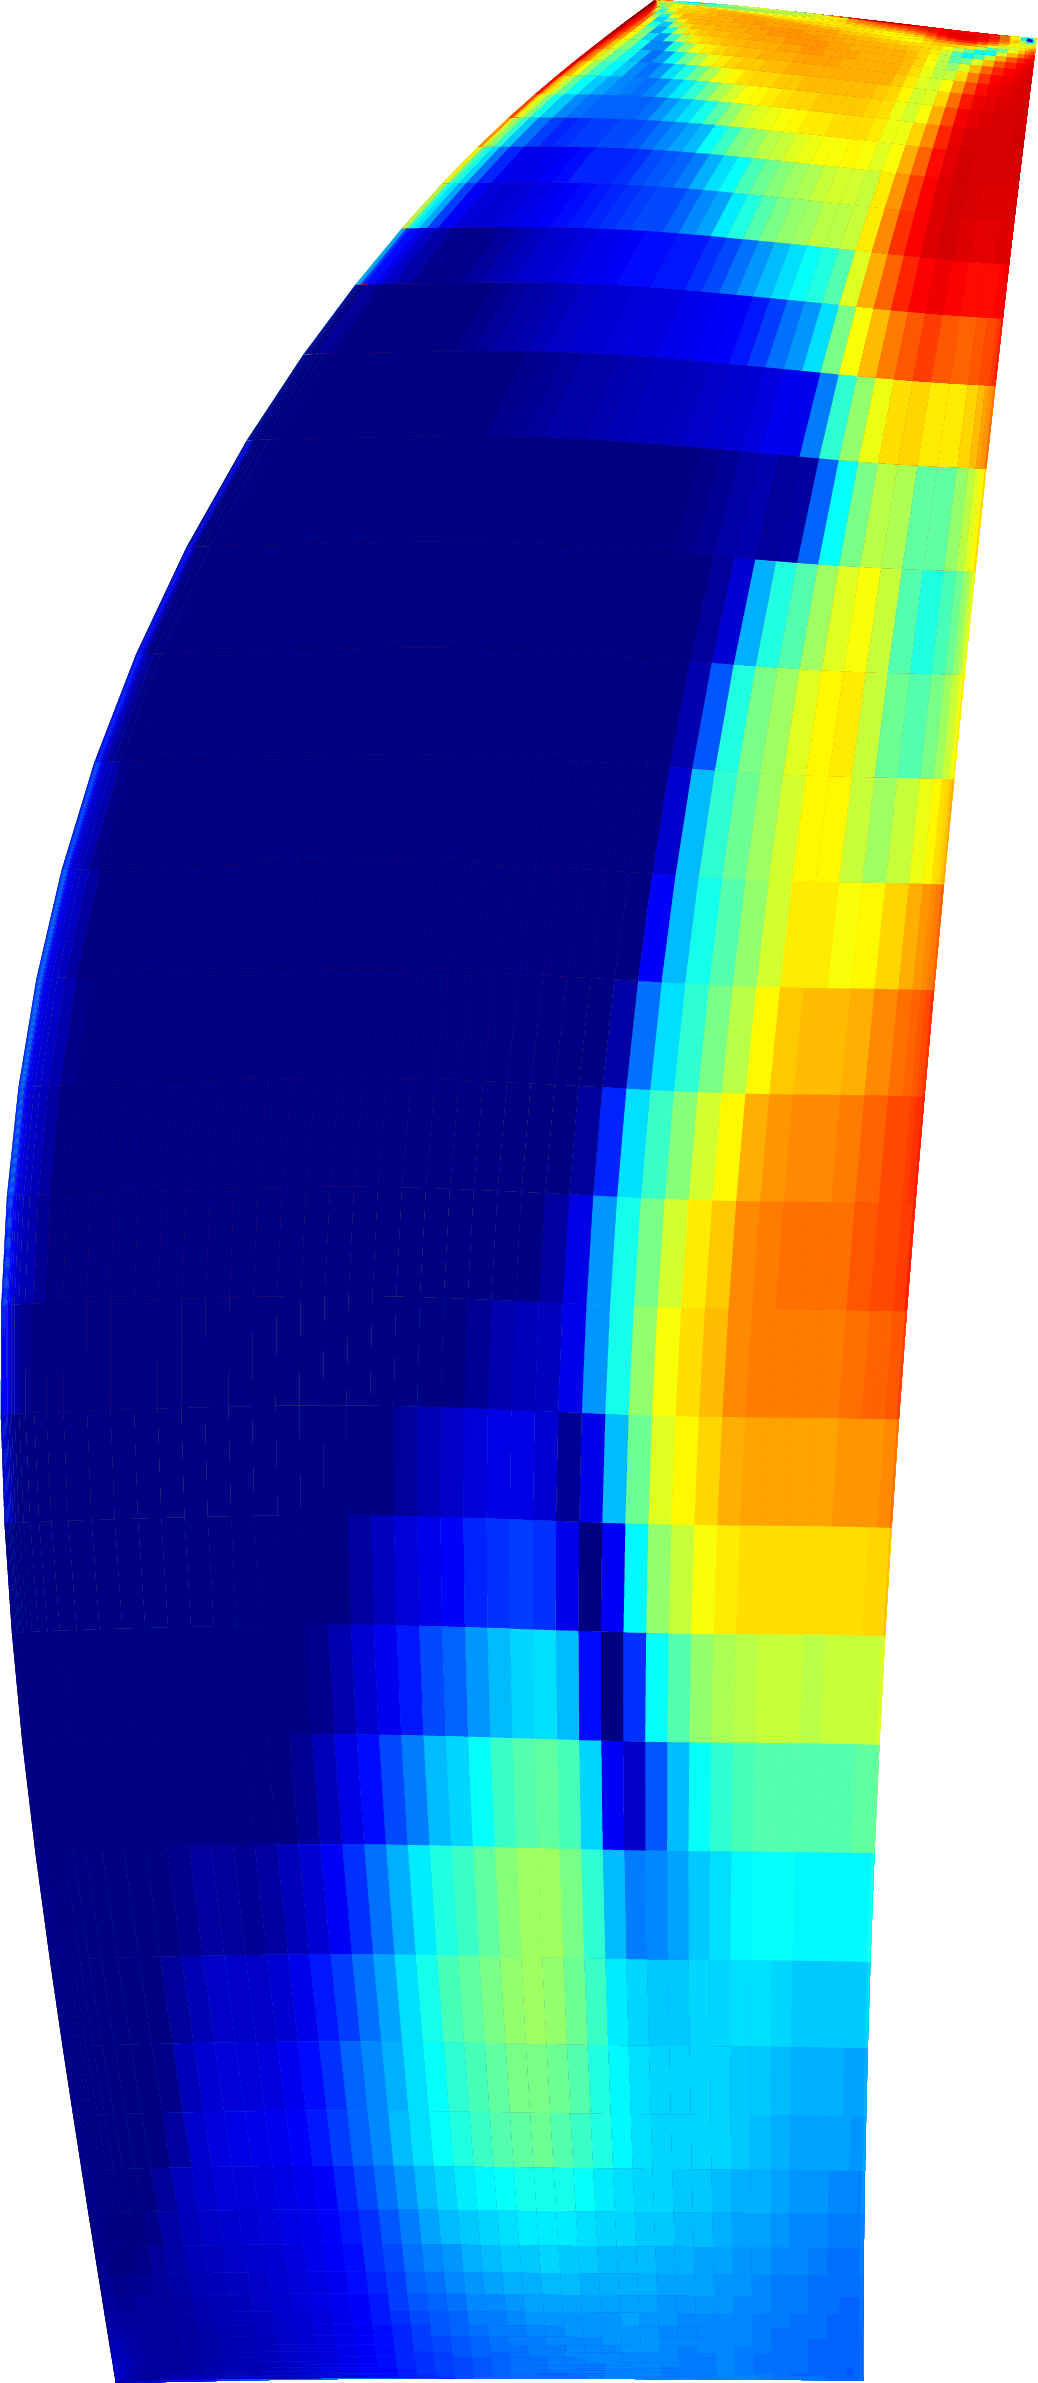
\includegraphics[width=0.15\textwidth]{DREAM_HS_TSM_N7_roe2_sa_blade_response_front_H01_SS.png}
    & 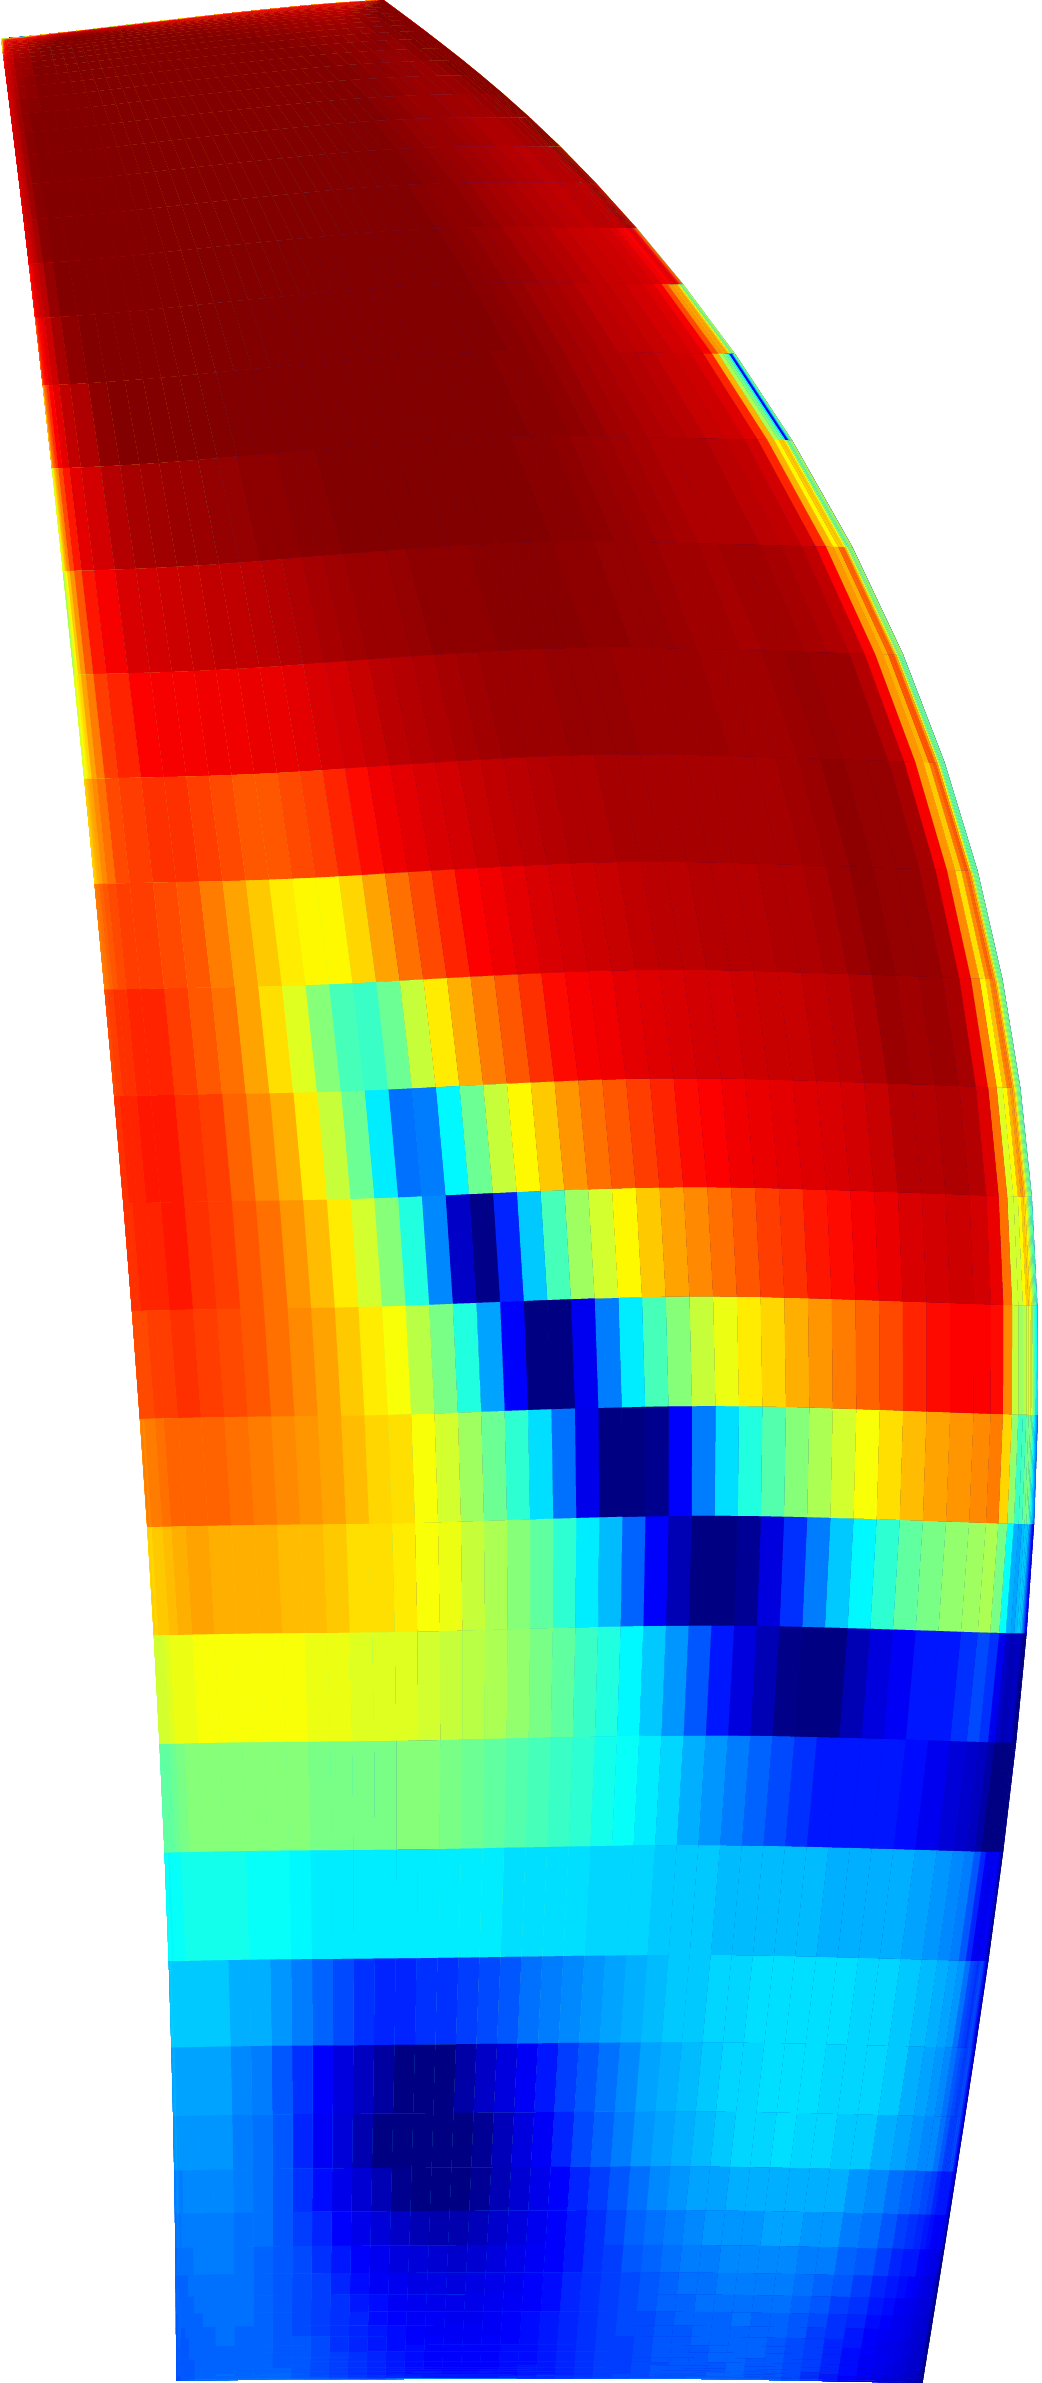
\includegraphics[width=0.15\textwidth]{DREAM_HS_TSM_N7_roe2_sa_blade_response_front_H01_PS.png}
    & 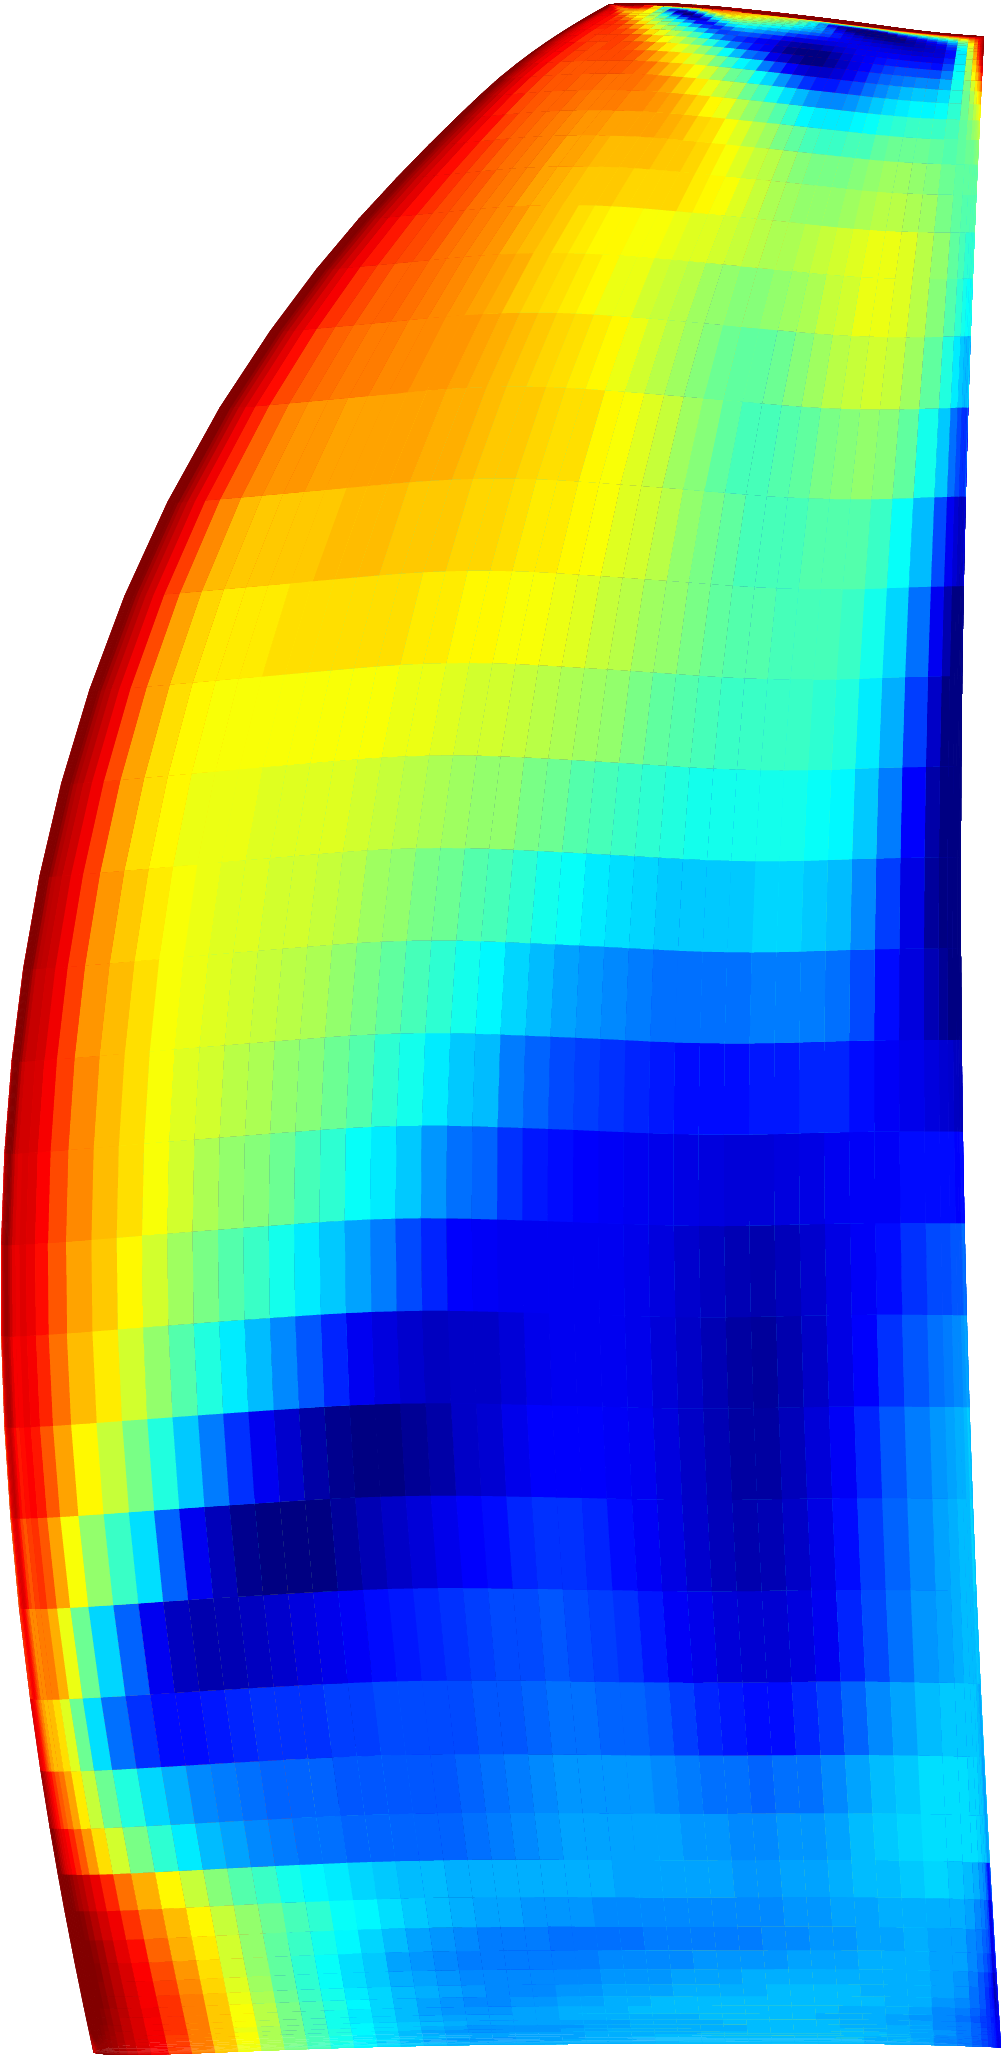
\includegraphics[width=0.15\textwidth]{DREAM_HS_TSM_N7_roe2_sa_blade_response_rear_H01_PS.png}
    & 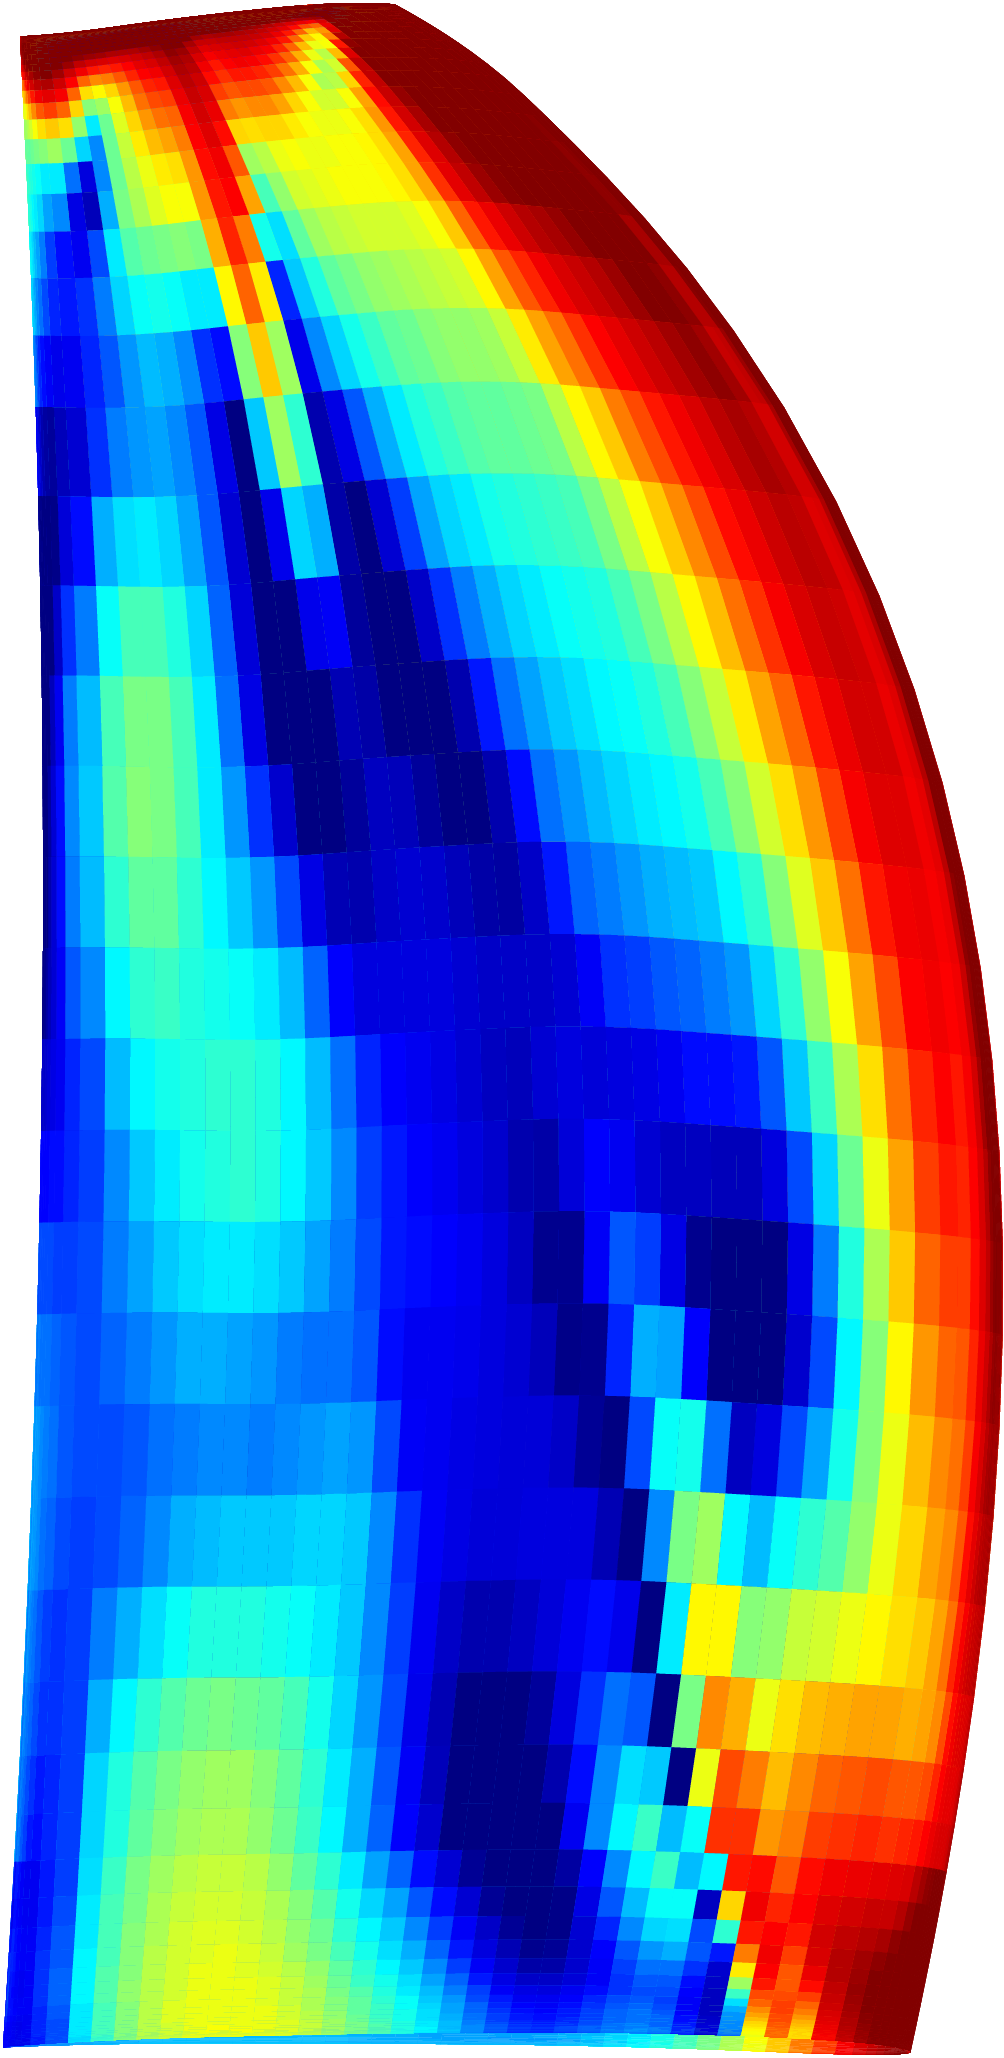
\includegraphics[width=0.15\textwidth]{DREAM_HS_TSM_N7_roe2_sa_blade_response_rear_H01_SS.png} \\
    \multicolumn{2}{c}{\emph{Front rotor blade}}
    & \multicolumn{2}{c}{\emph{Rear rotor blade}} \\
    suction side & pressure side & pressure side & suction side
 \end{tabular}
 \caption{High-speed isolated configuration: harmonic response of the front
 rotor blades.}
 \label{fig:dream_hs_hb_blade_response}
\end{figure}

On the front rotor, the maximum amplitude
is observed at the tip of the pressure side. This is consistent
with the observation made on the low-speed configuration, where
the pressure side was more exposed to pressure variations.
In fact, the suction side is shielded by the blade angle of attack
from downstream disturbances.
The suction side is not only shielded by the blade angle
of attack but also by the shock that forms around 
$x/c \approx 0.7$ for relative span greater than $40\%$,
as mentioned in Sec.~\ref{sub:dream_hs_blades}. For
relative span smaller than $40\%$, the shock is closer the
leading edge, hence the pressure unsteadiness that goes
upstream. On the tip of the front rotor blade,
a vortex is formed that leaves the blades from the pressure
side to the suction side. It helps increasing
the pressure on the suction side, alleviating the formation
of a shock. Therefore, at the tip of the blade, the pressure variations
are observed all the way to the leading edge.

On the rear rotor, the suction side of the blade 
shows a large structure of high unsteadiness near 
the leading edge. This is attributed to the wake passing.
In opposite, a large low amplitude region is observed in the
middle of the suction side of the blade. This is attributed
to the shielding effect of the shock. In fact, the shock is 
a discontinuity that prevents unsteady effects to affect the
blade. On the pressure side, the level of unsteadiness is much larger
than the one observed on the low-speed configuration, relatively
to the suction side level. Actually, the smaller
angle of attack of the blades might explain this high level.
Similar as the suction side of the front rotor
blade that are shielded from potential effects coming
from the rear rotor blades, the pressure side is relatively
less affected by the wake passing than the suction side is.
However, for the high-speed configuration, the angle of
attack is smaller as said in Sec.~\ref{sec:dream_hs_presentation}.
Therefore, the unsteady effects hitting the suction side of the
rear rotor blades are more prone to affect the pressure side
too. Moreover, as no shock is present on the pressure side,
these unsteadinesses affects the whole chord. This is
the author's interpretation.

\subsection{Two-dimensional results: axial cuts}
\label{sub:dream_hs_hb_axial_cuts}

Axial cuts of entropy are shown in 
Fig.~\ref{fig:dream_hs_hb_axial_cut_entropy} for several
axis positions and compared to steady computation results.
\begin{figure}[htp]
 \ra{1.3} \centering
 \begin{tabular}{rcc}
   & steady
   & HB $N=4$ \\
   \rotatebox{90}{\qquad\qquad\qquad $P3$} & 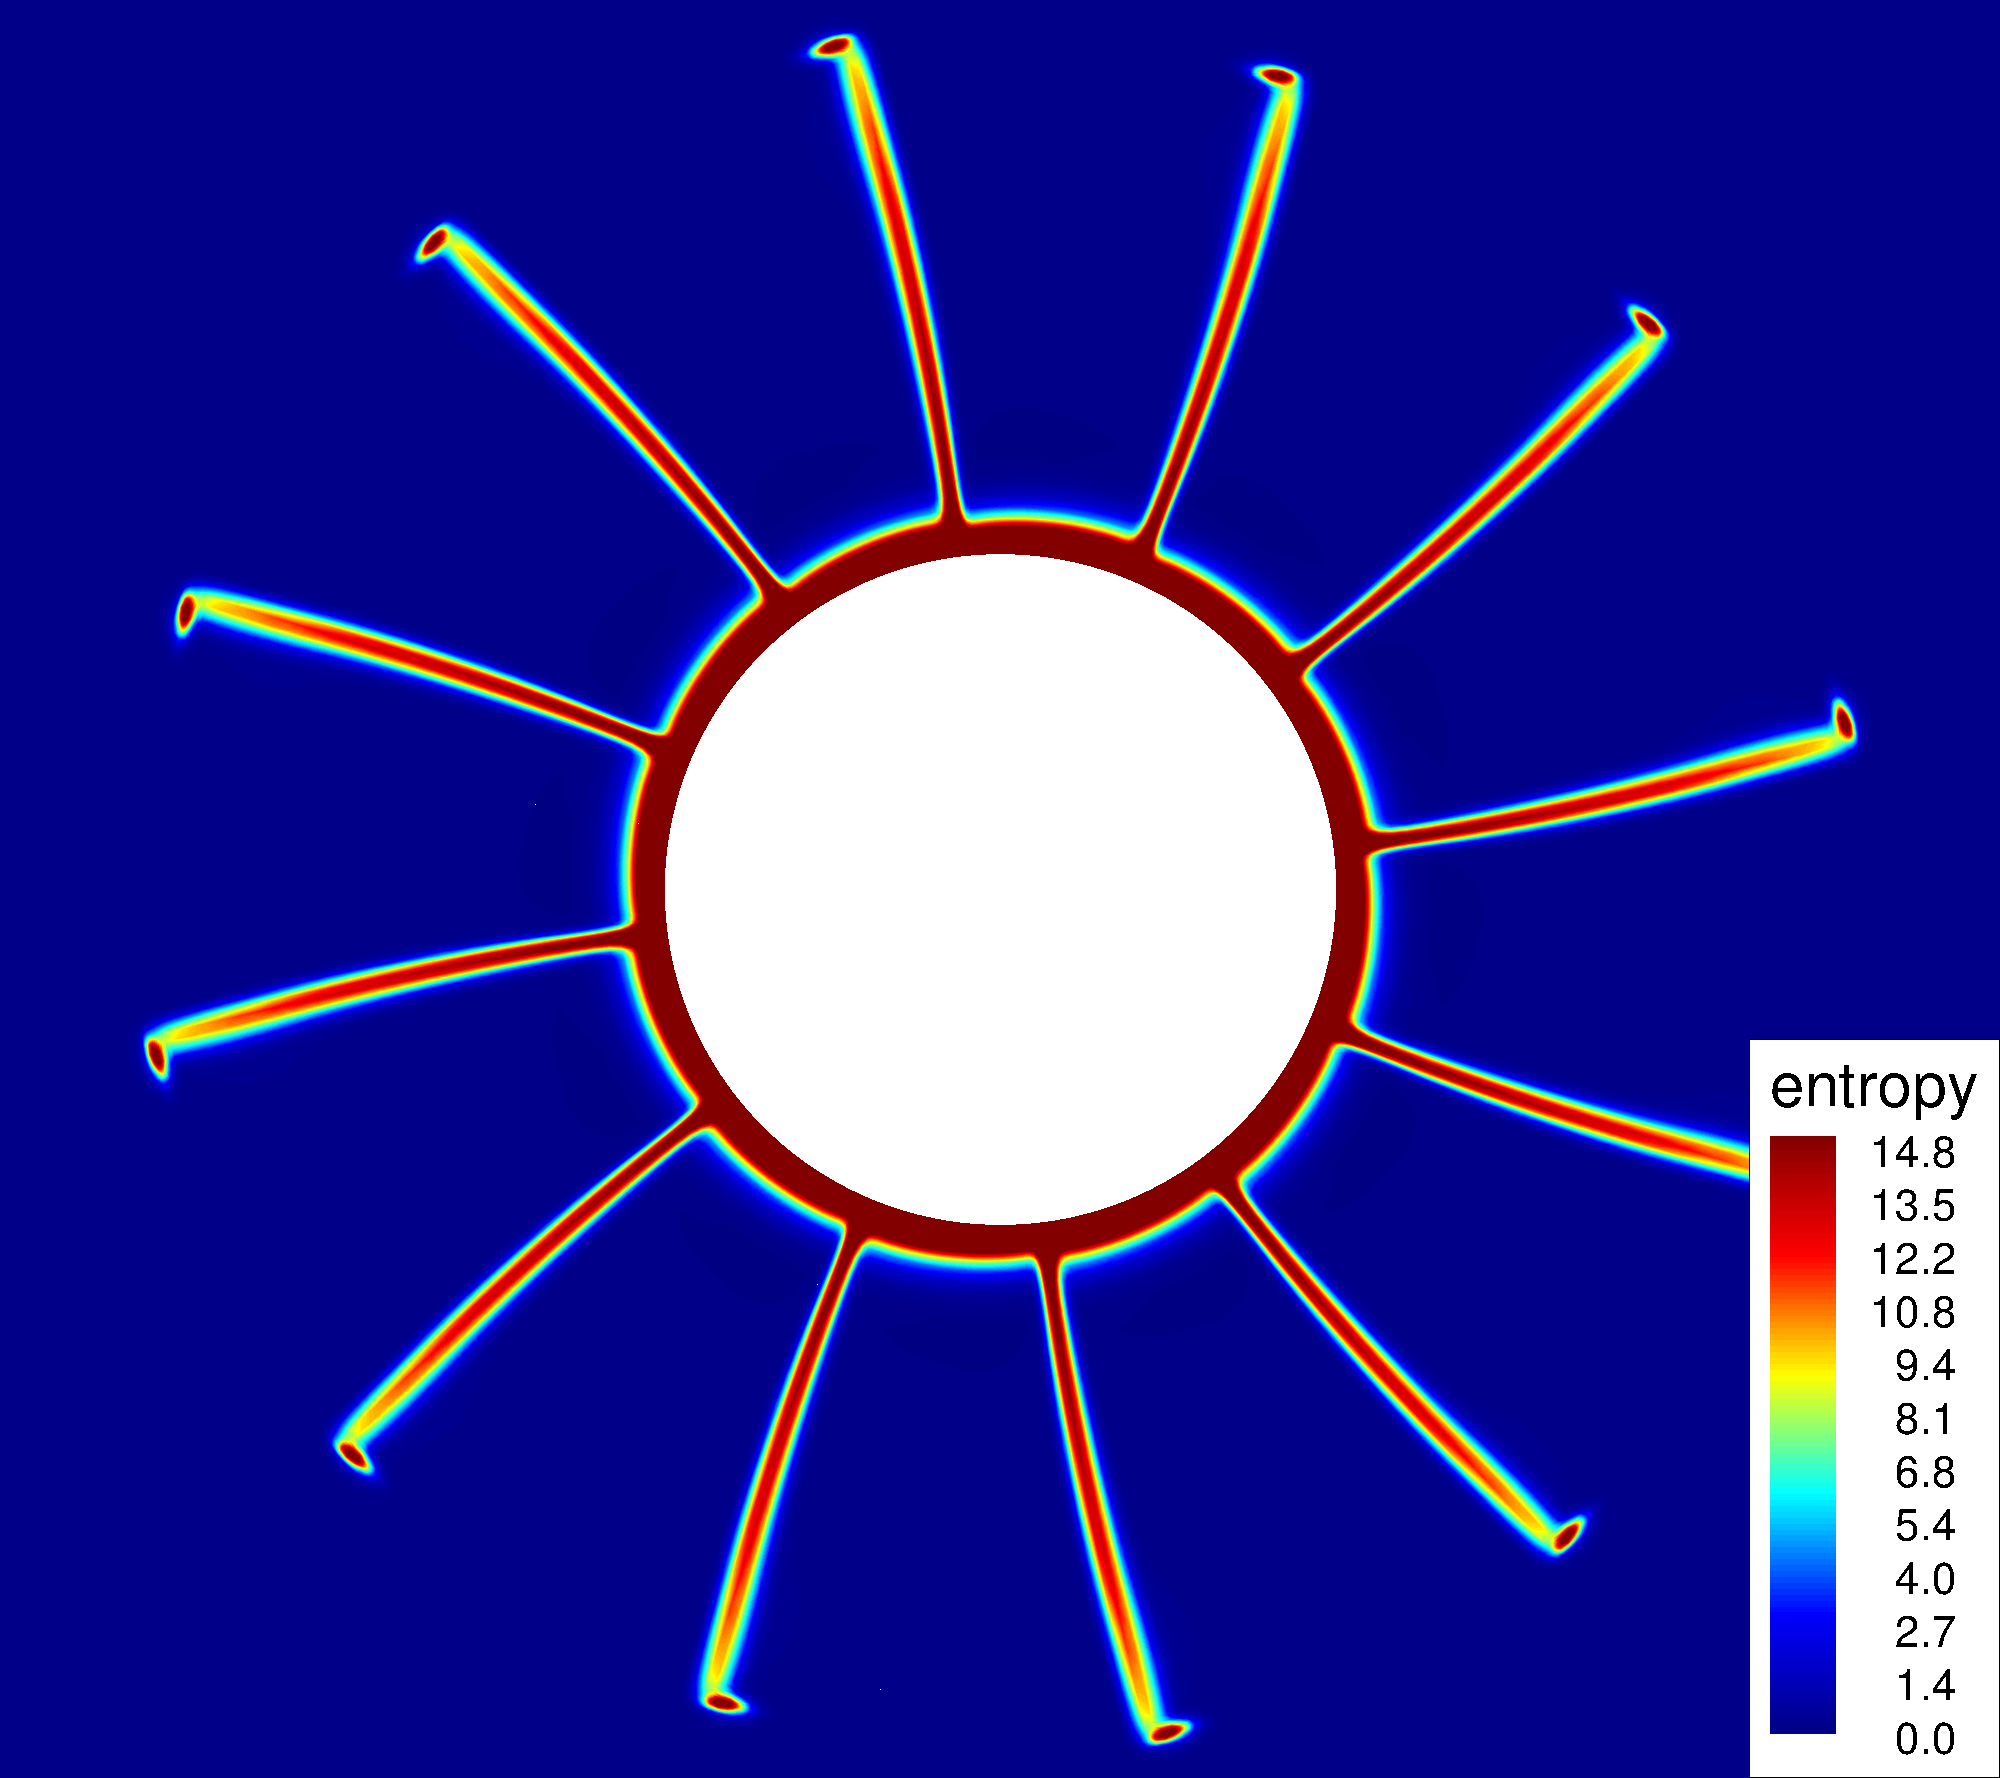
\includegraphics[width=.35\textwidth]{DREAM_HS_RANS_roe2_sa_slice_x_front_1_entropy.png}
   & 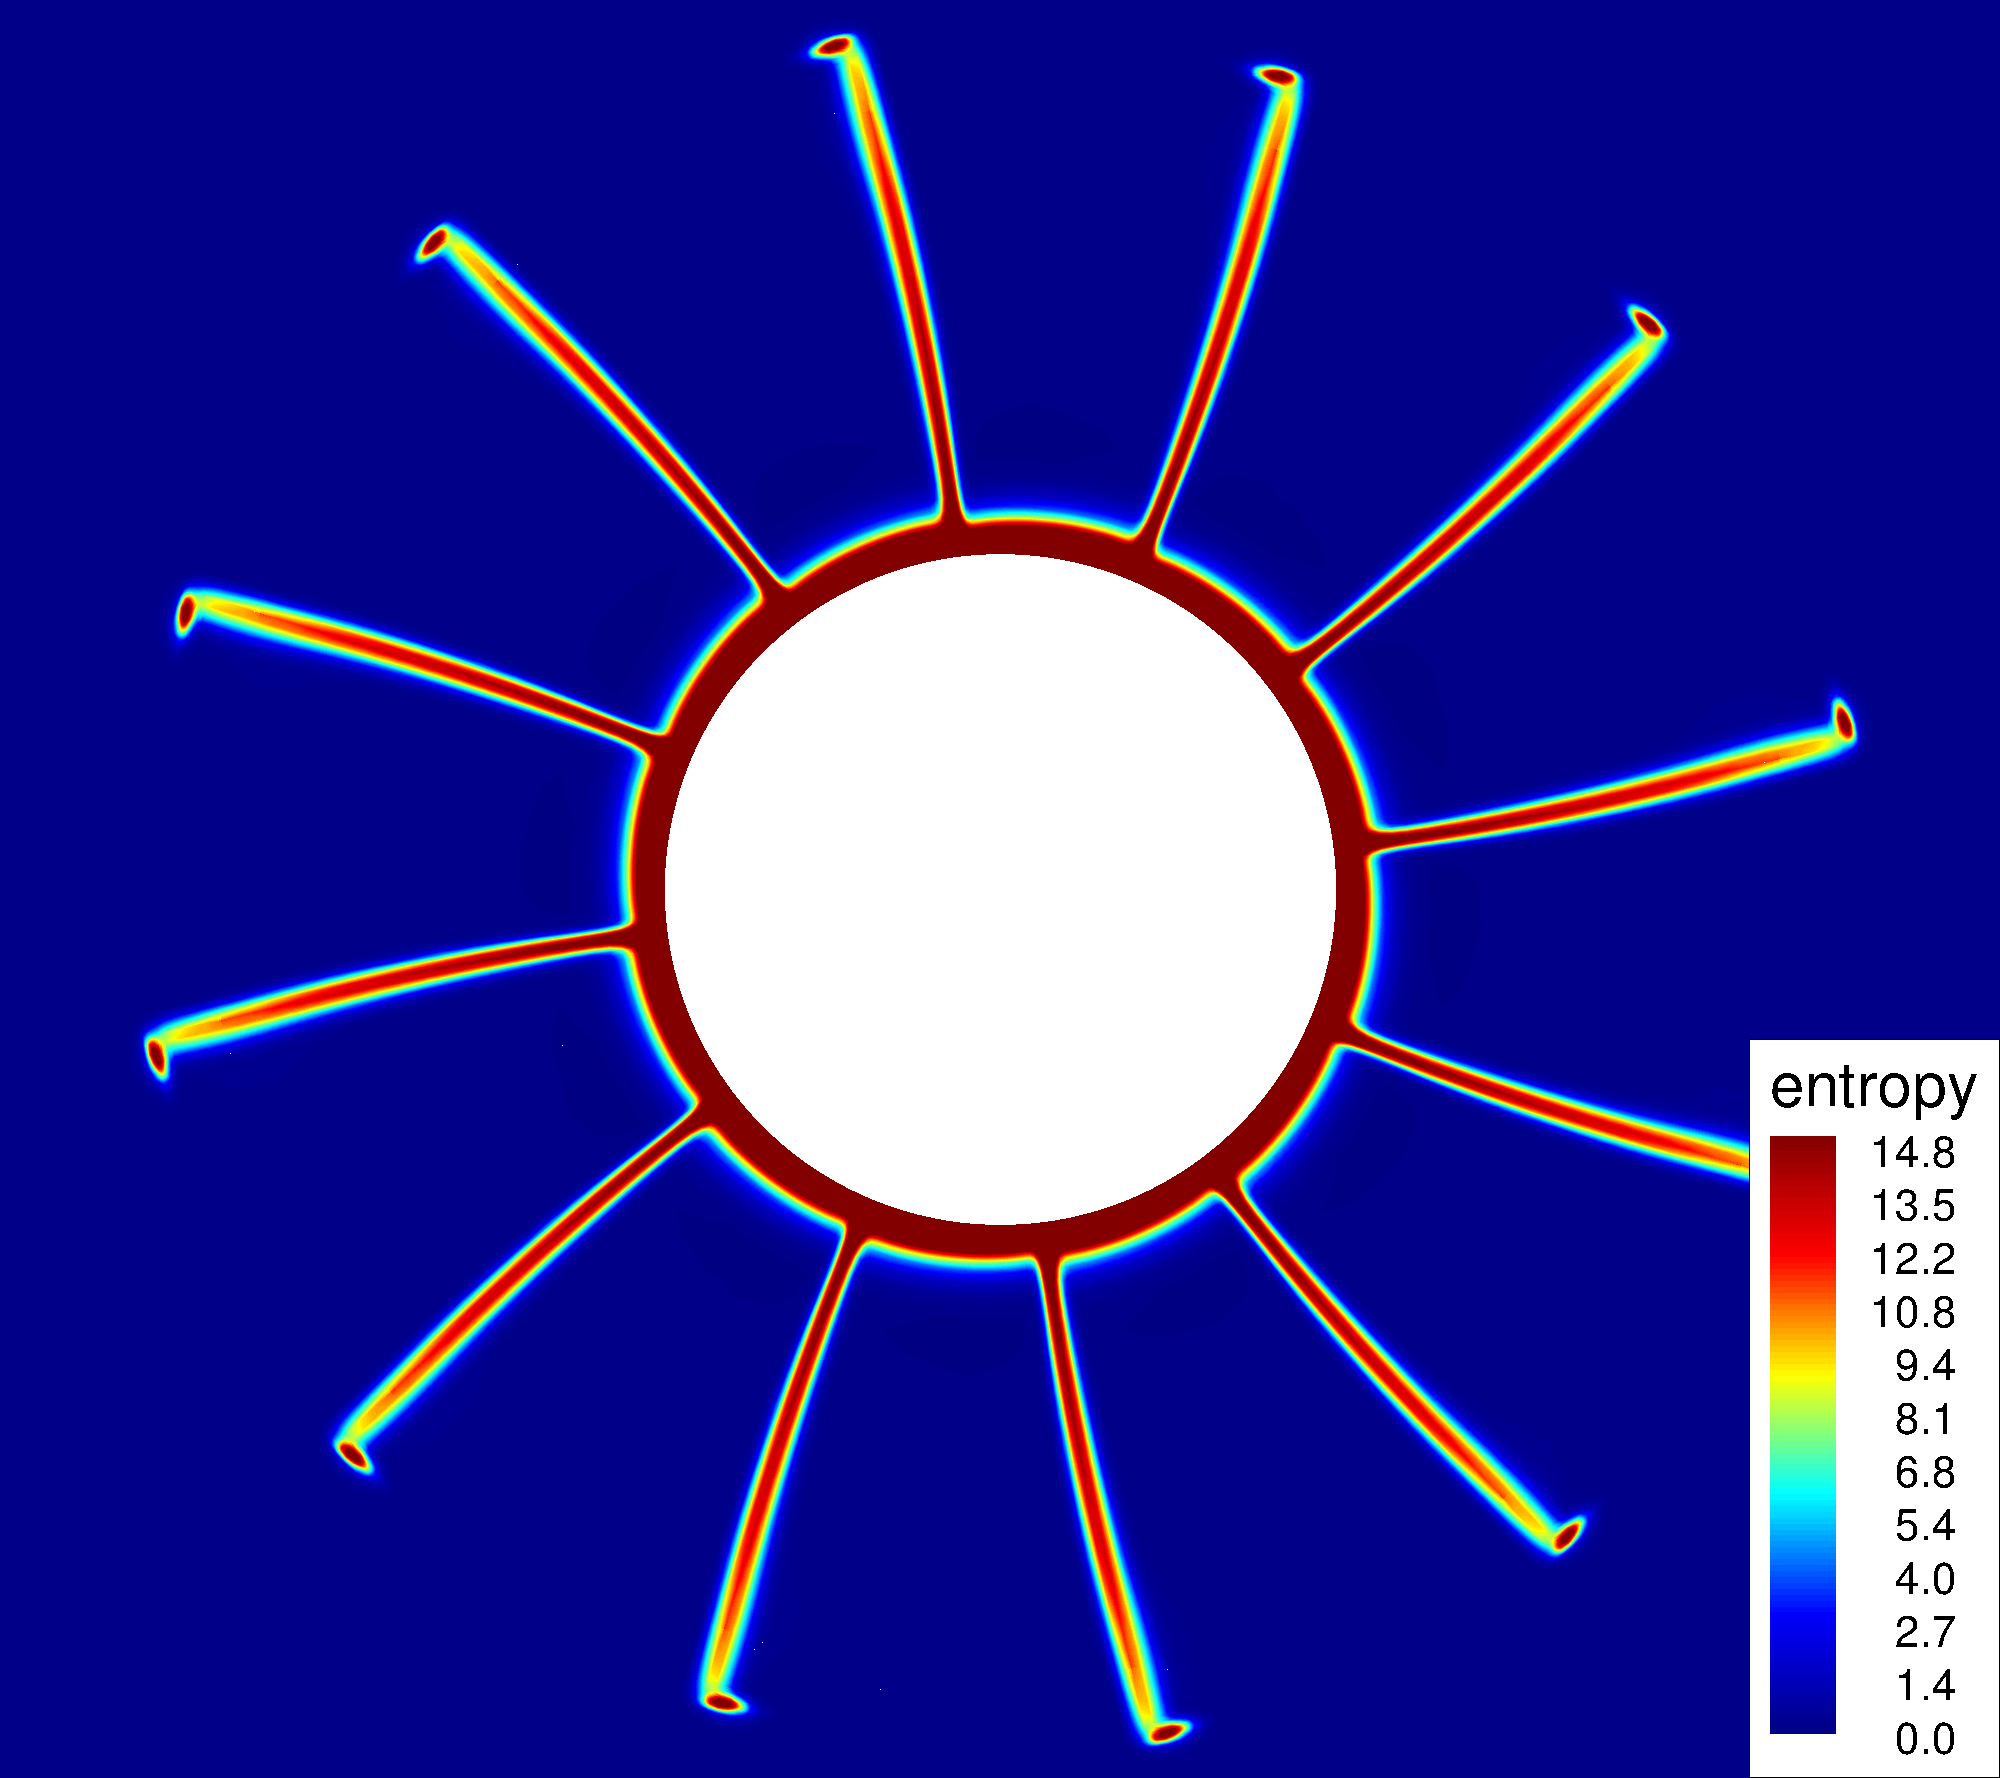
\includegraphics[width=.35\textwidth]{DREAM_HS_TSM_N7_roe2_sa_slice_x_front_1_entropy.png} \\
   \rotatebox{90}{\qquad\qquad\qquad $P4$} & 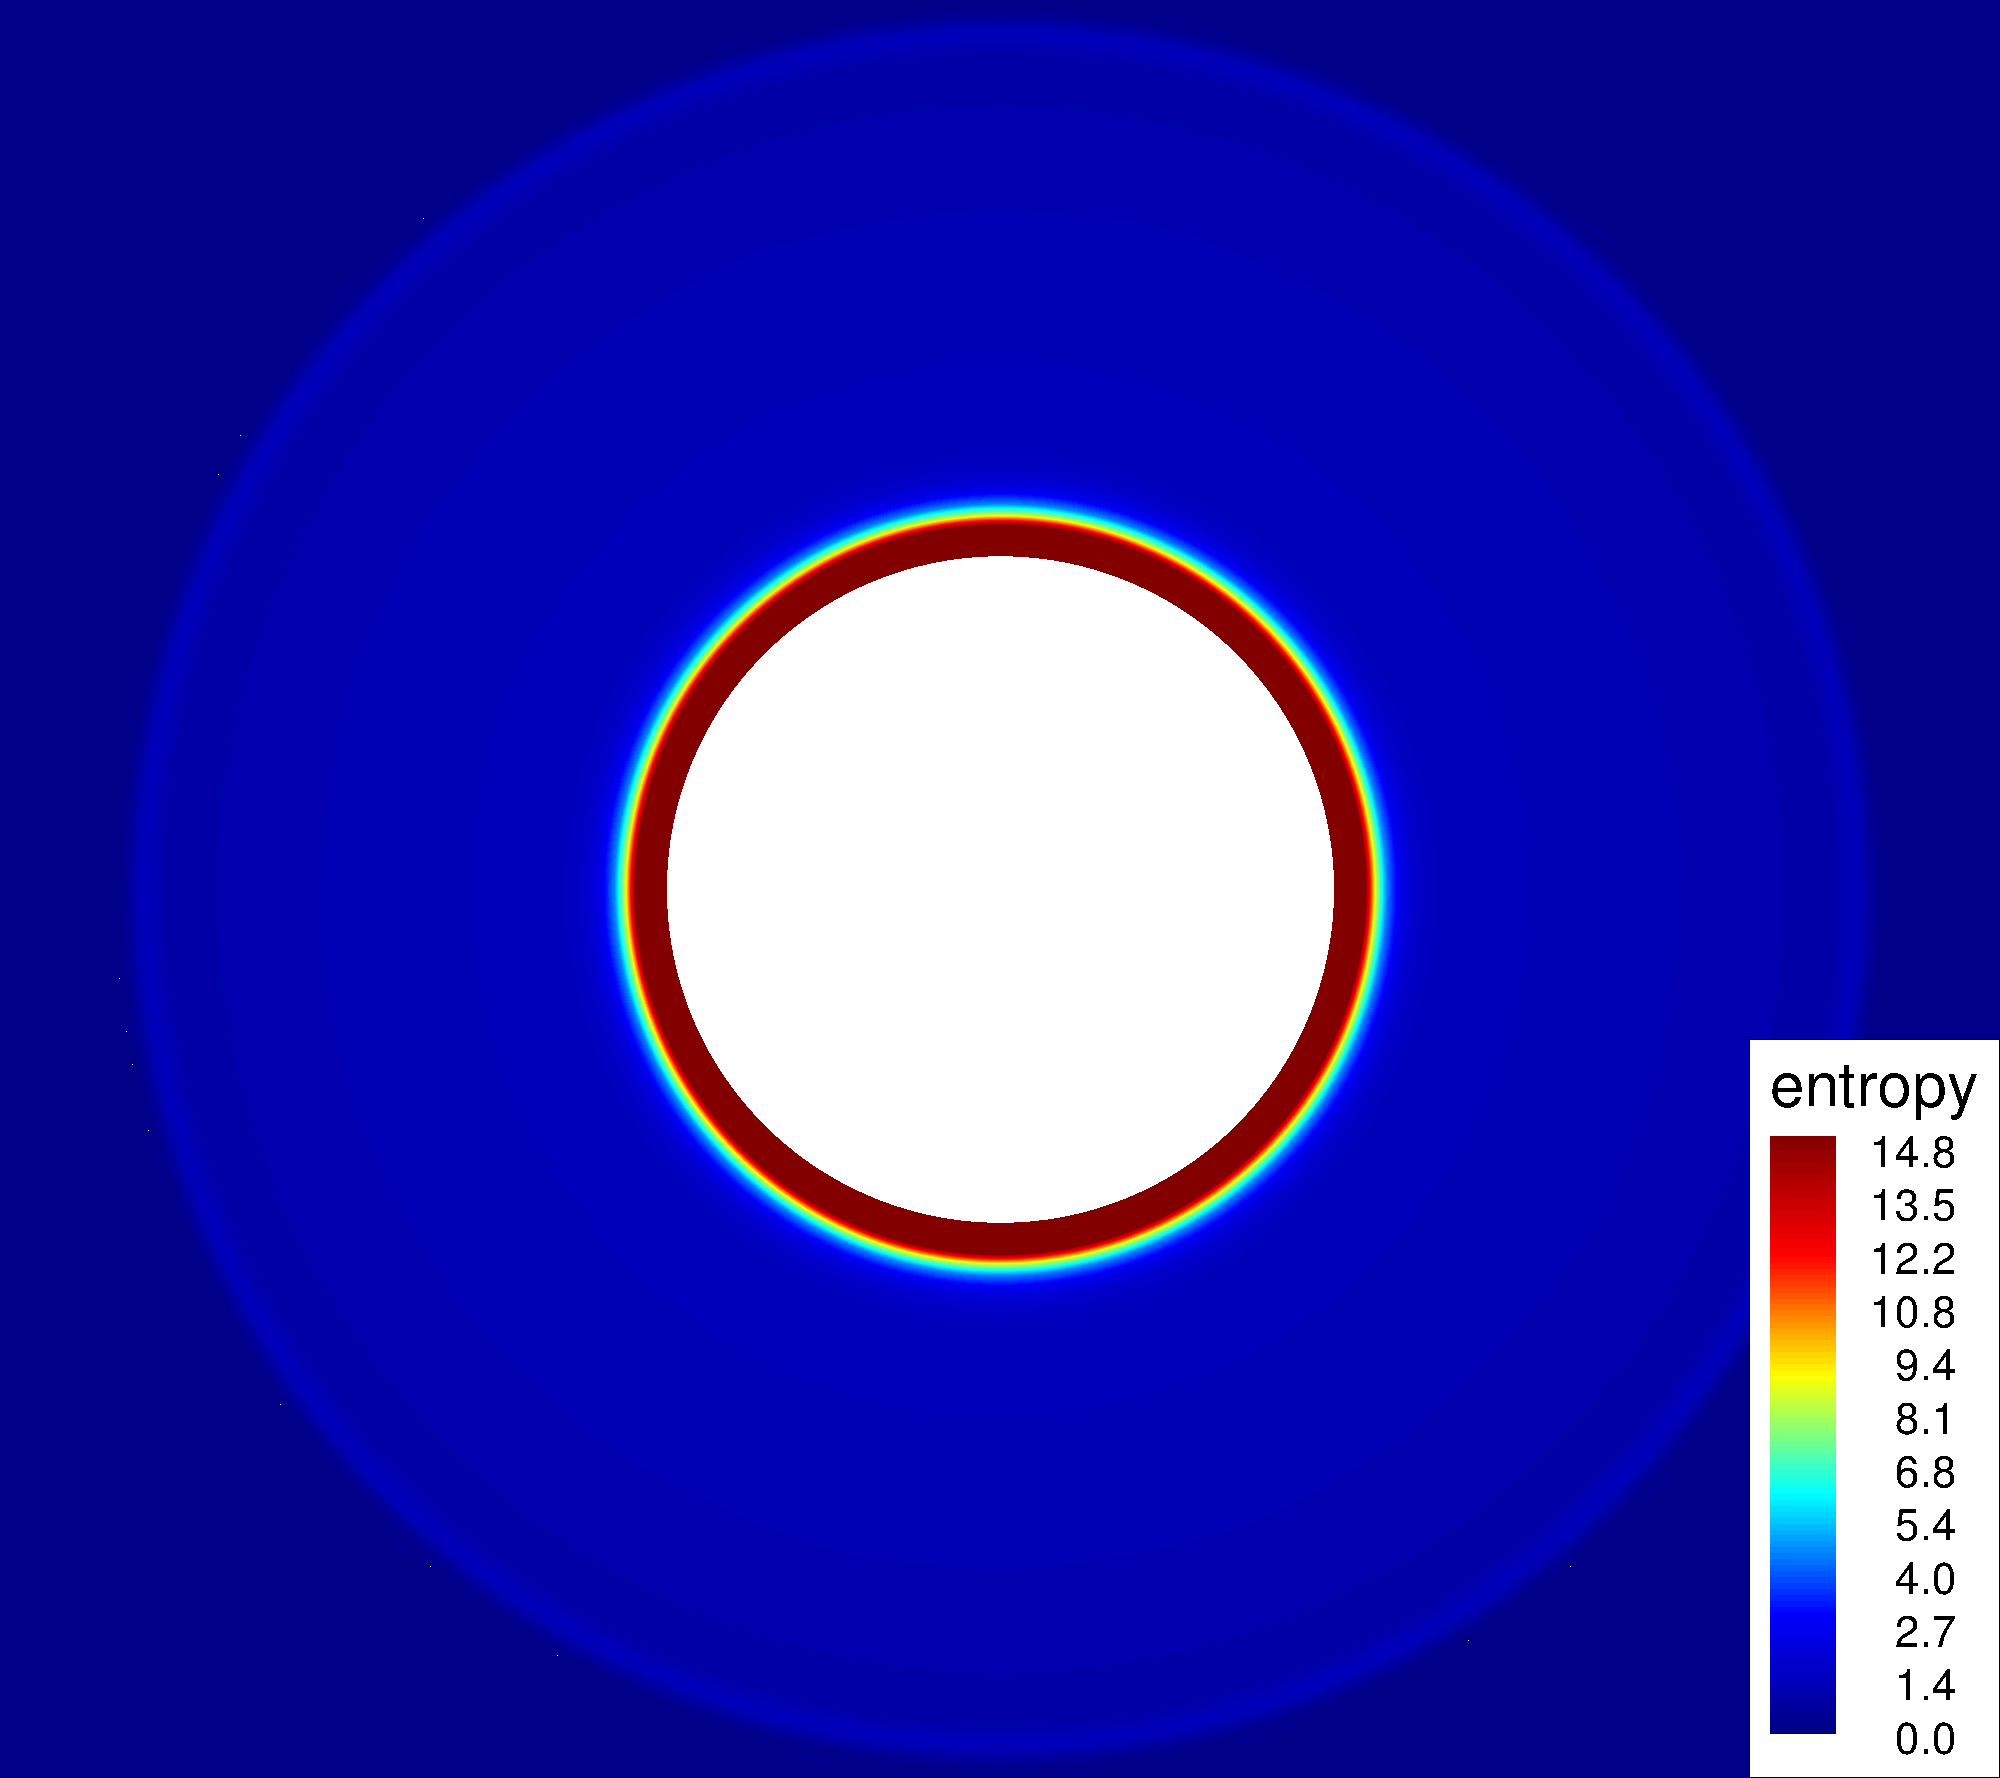
\includegraphics[width=.35\textwidth]{DREAM_HS_RANS_roe2_sa_slice_x_rear_0_entropy.png}
   & 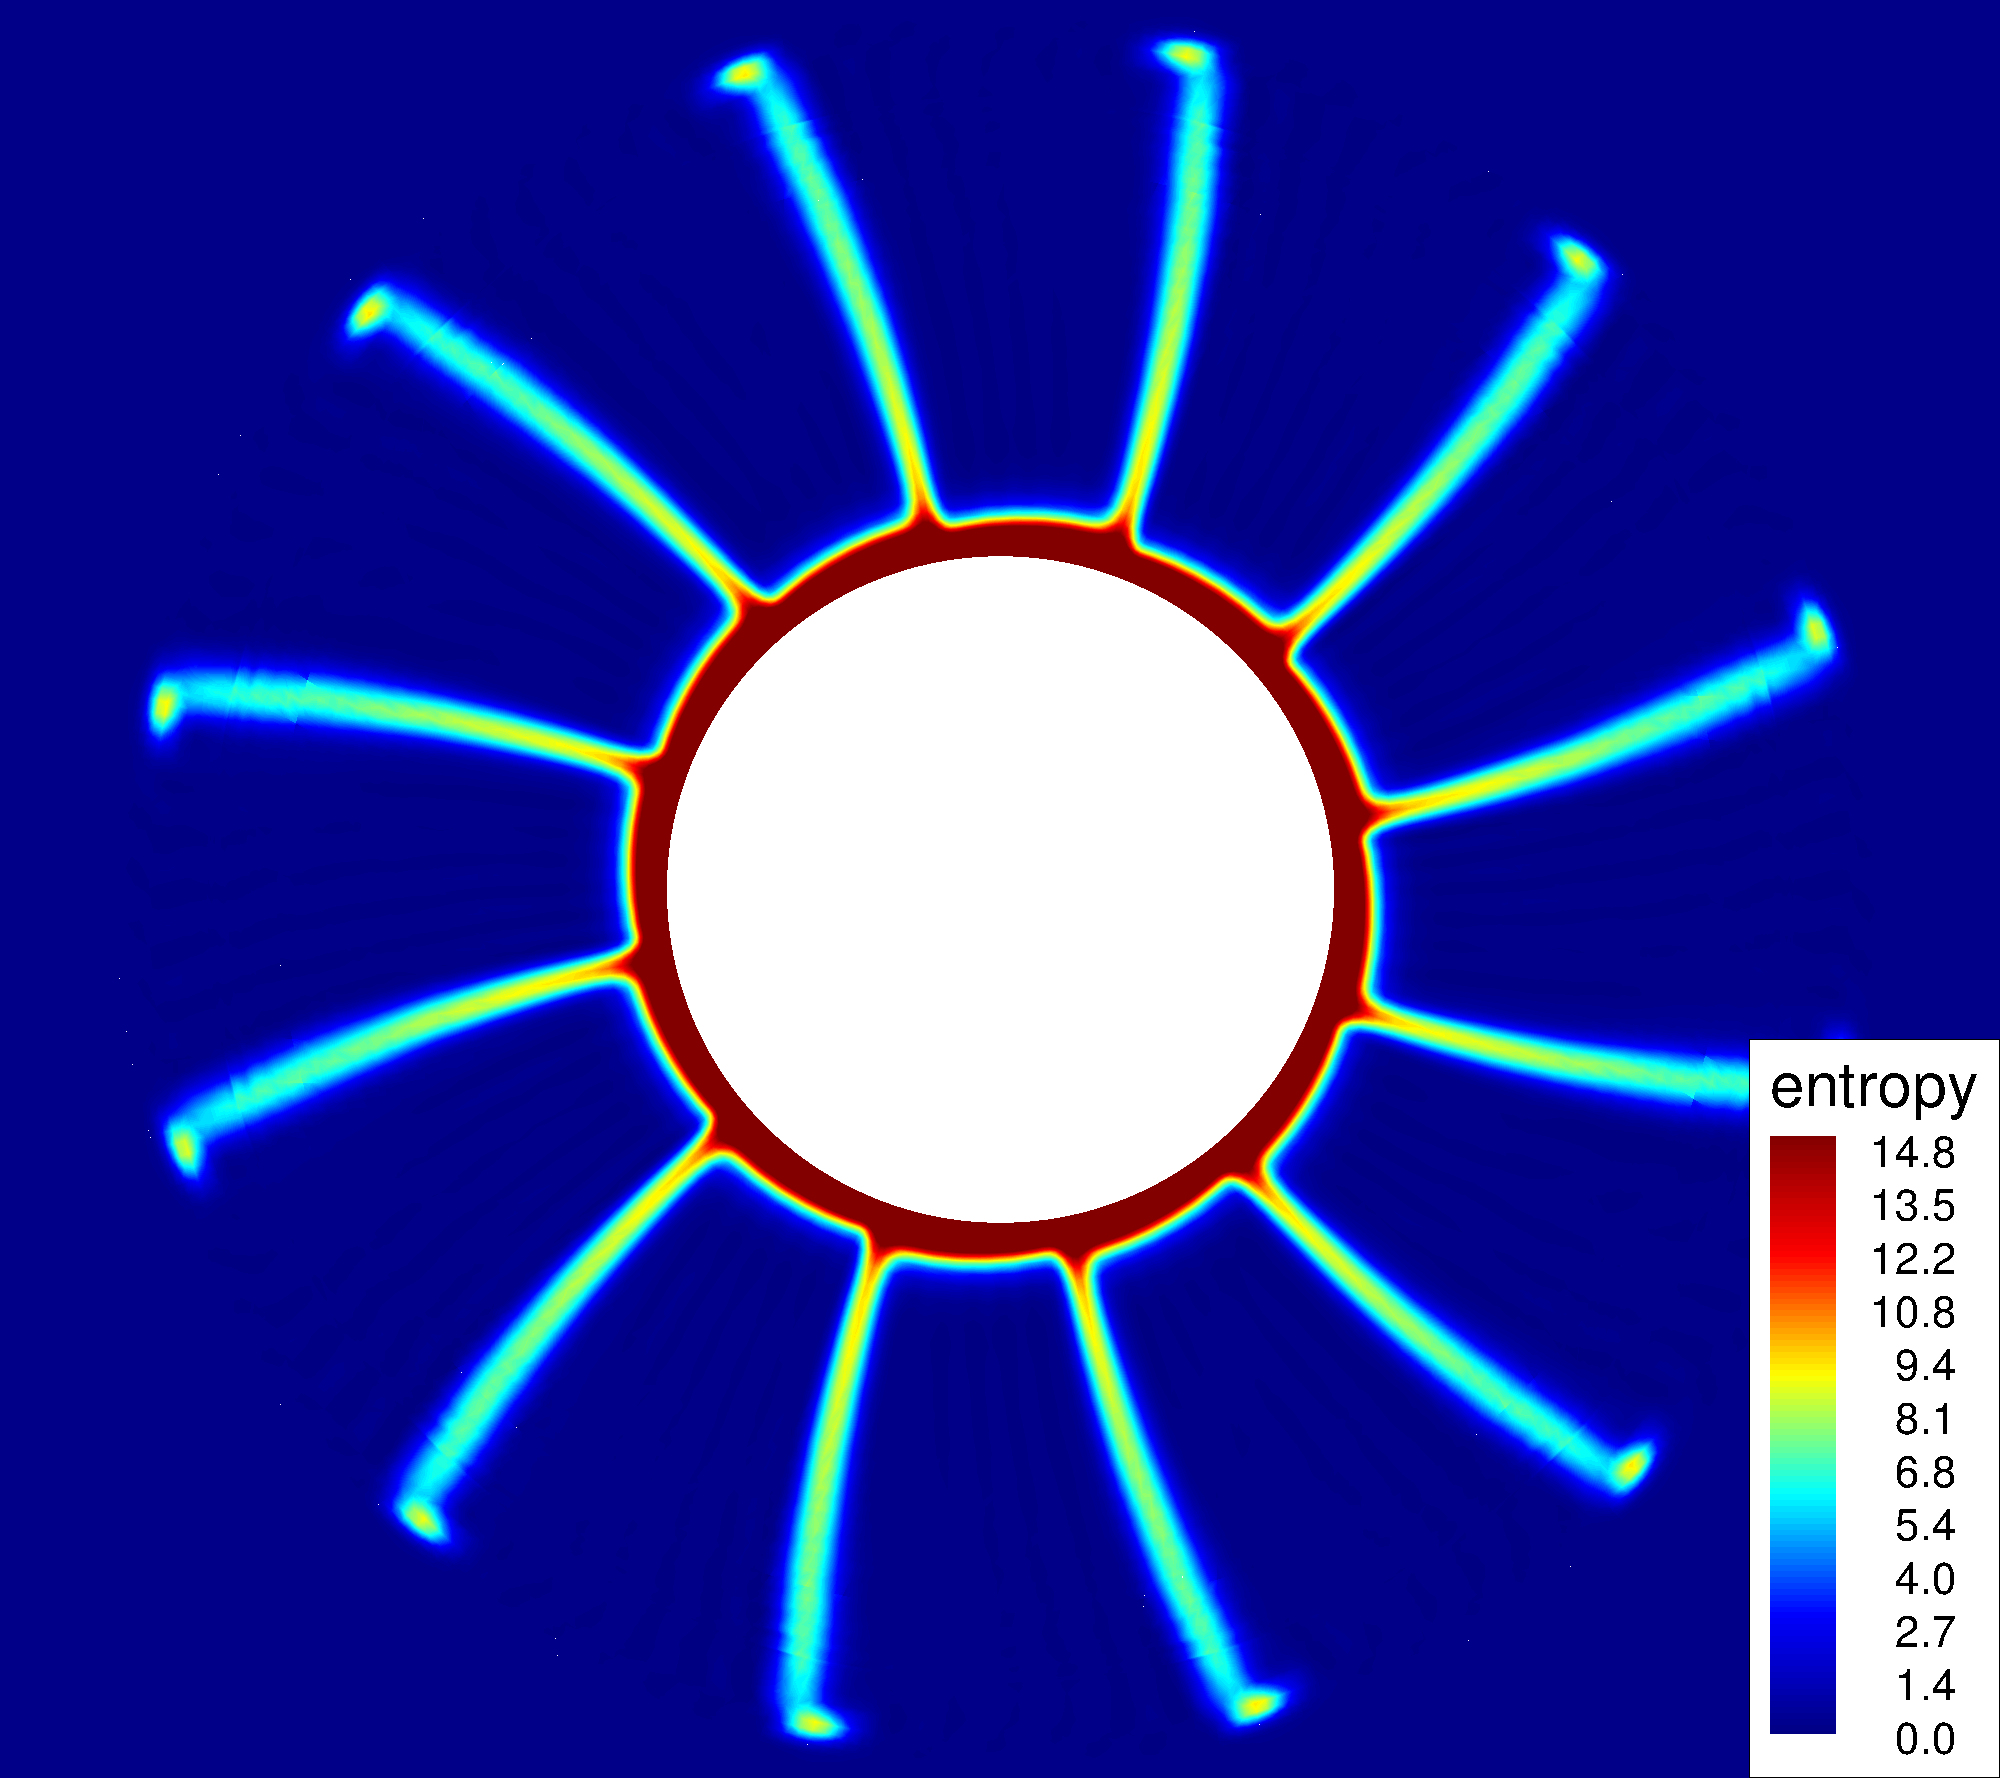
\includegraphics[width=.35\textwidth]{DREAM_HS_TSM_N7_roe2_sa_slice_x_rear_0_entropy.png} \\
   \rotatebox{90}{\qquad\qquad\qquad $P5$} & 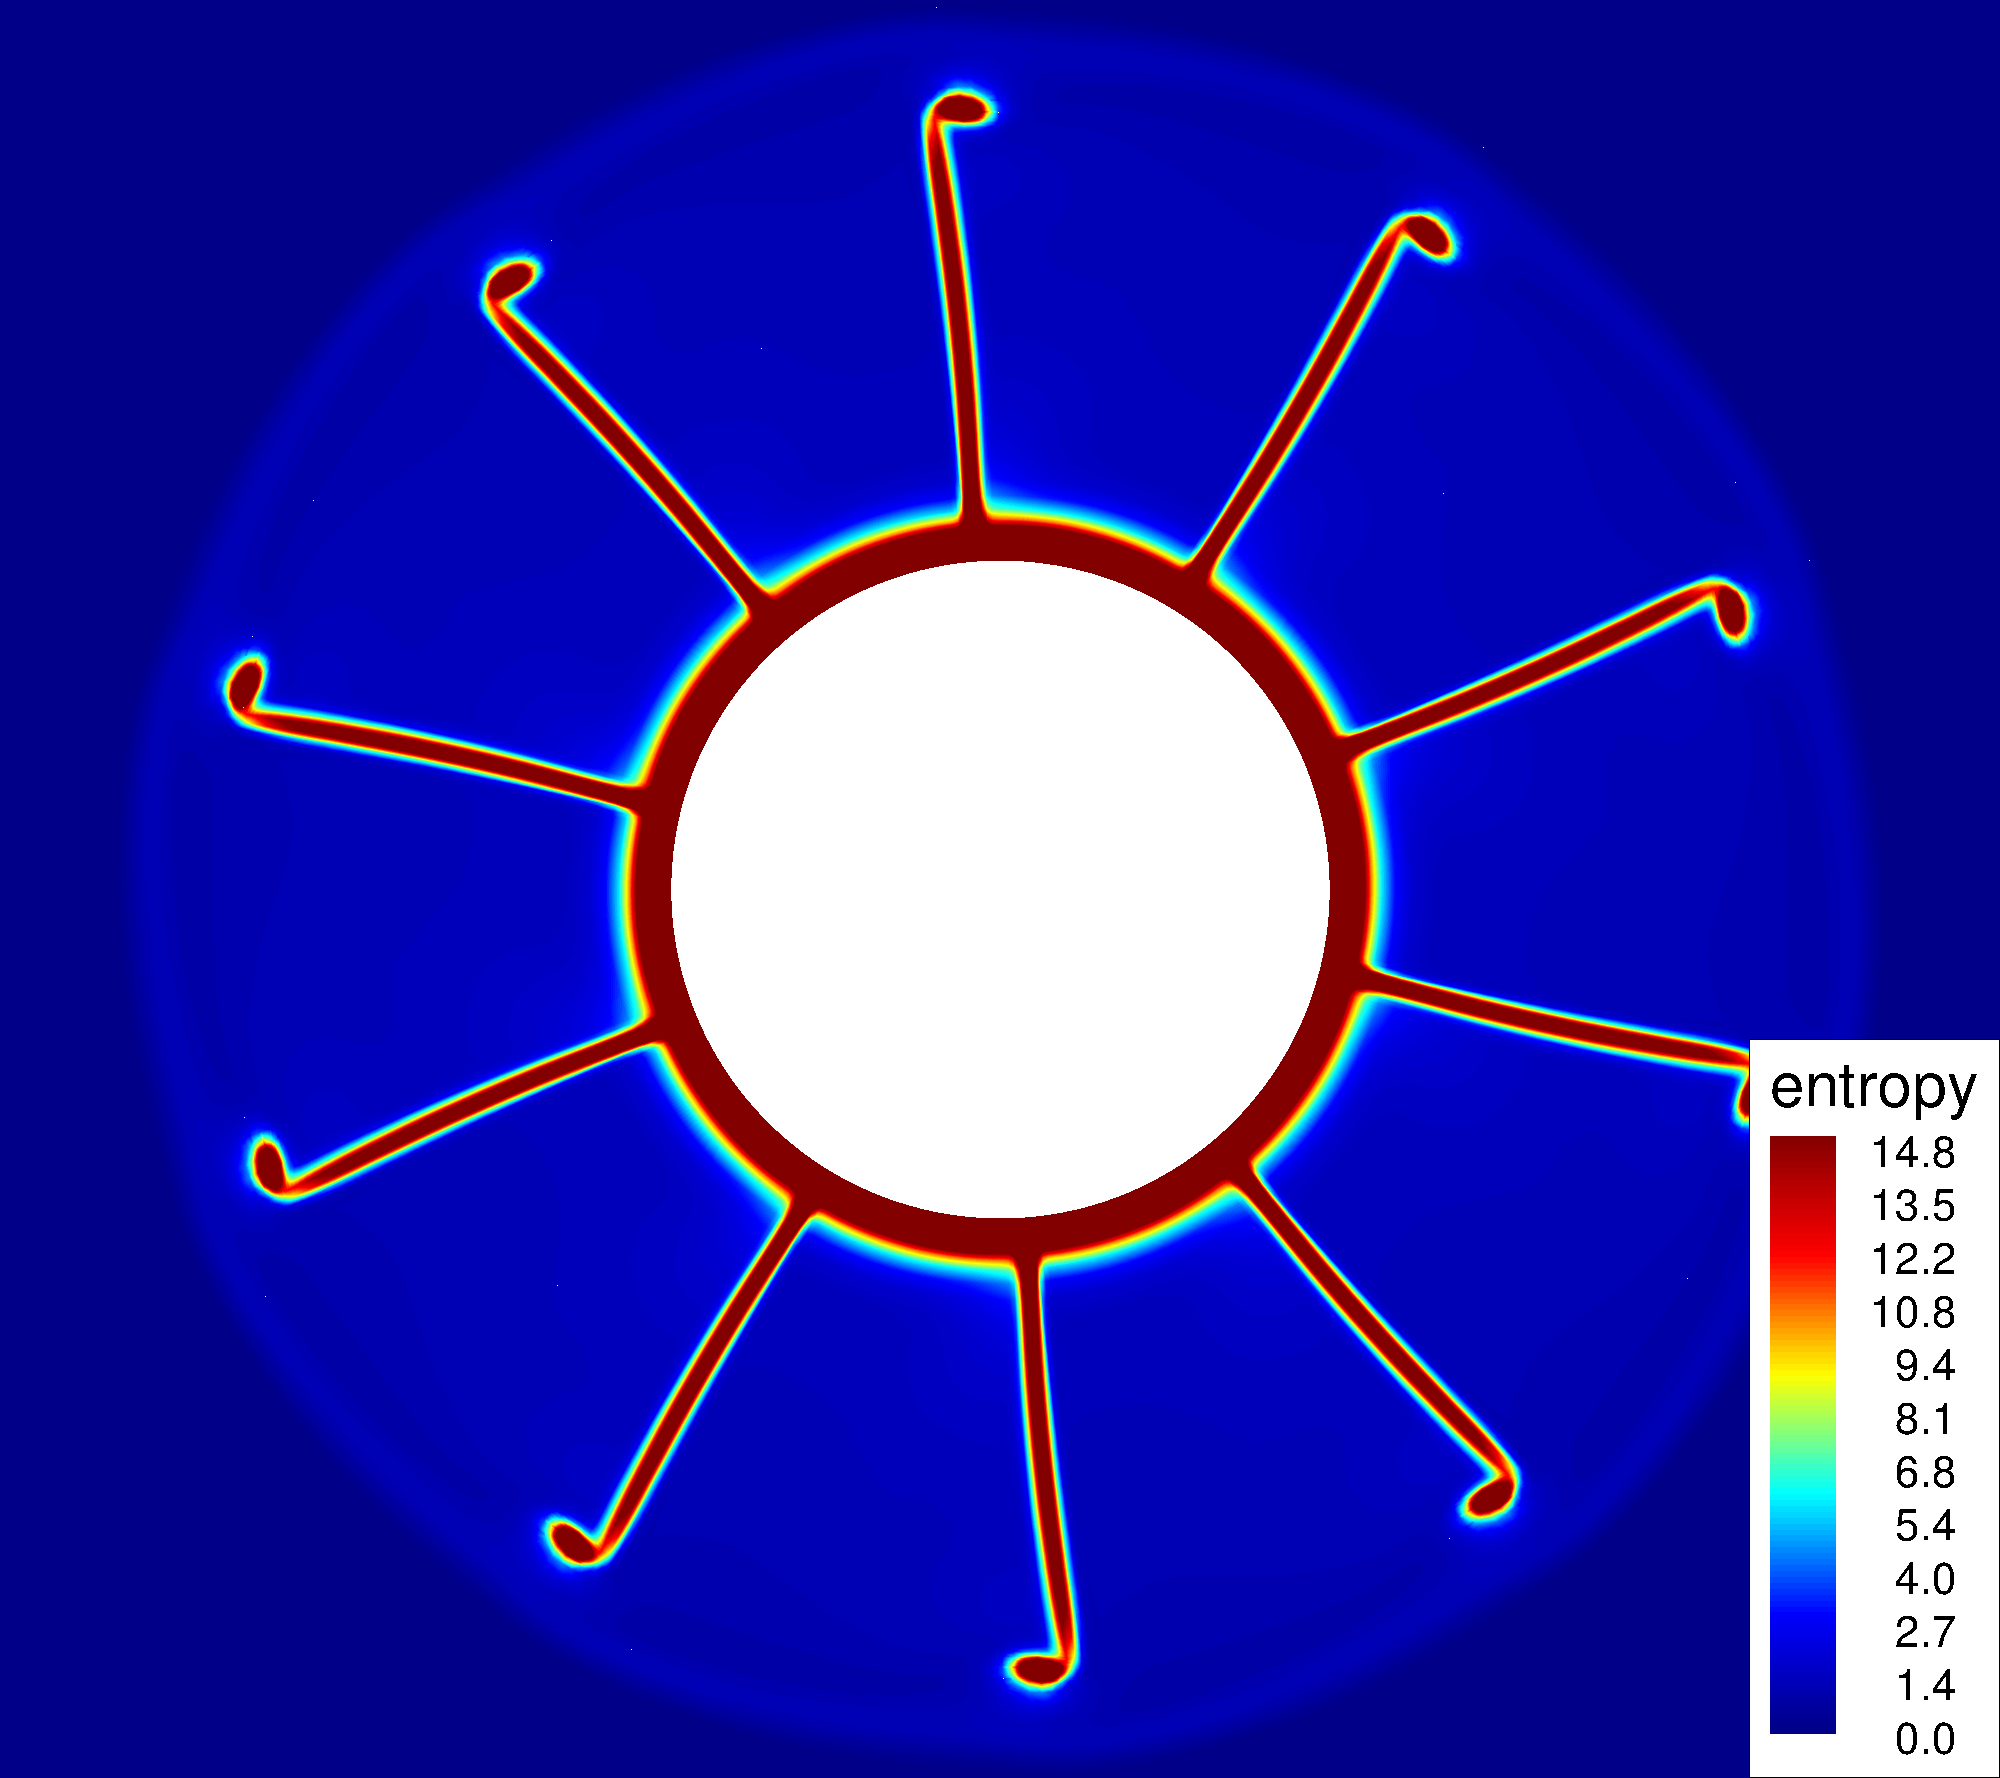
\includegraphics[width=.35\textwidth]{DREAM_HS_RANS_roe2_sa_slice_x_rear_1_entropy.png}
   & 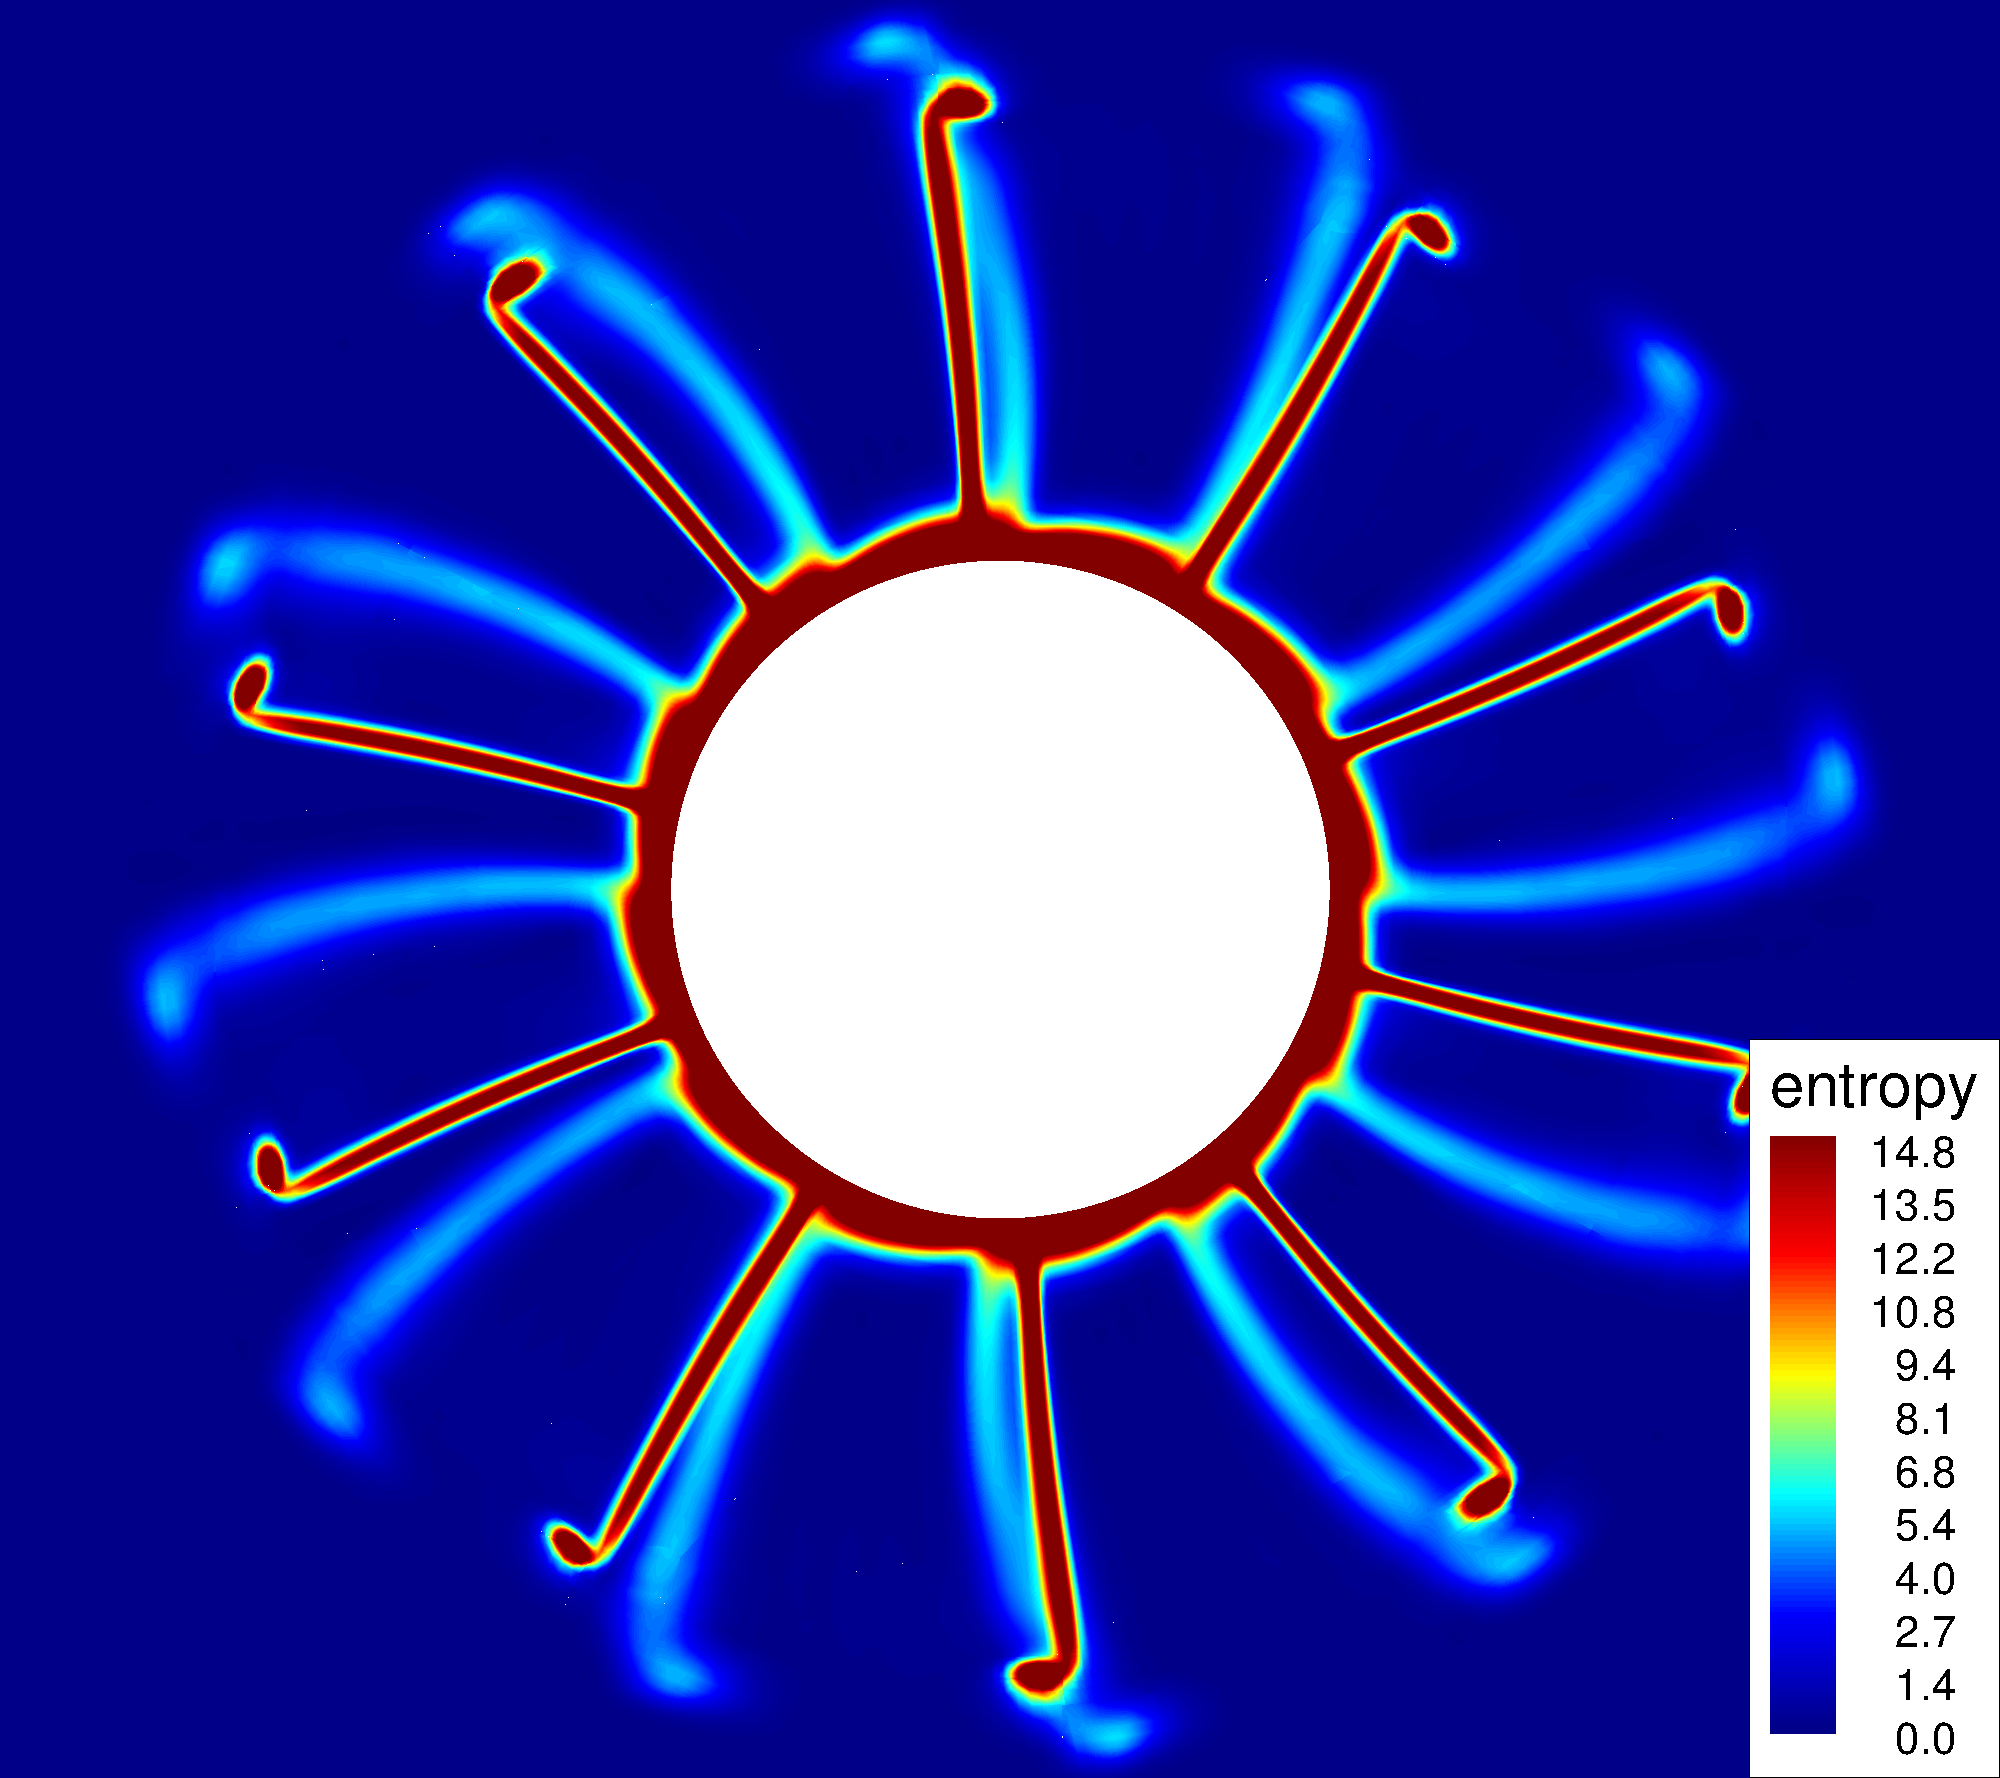
\includegraphics[width=.35\textwidth]{DREAM_HS_TSM_N7_roe2_sa_slice_x_rear_1_entropy.png} \\
   \rotatebox{90}{\qquad\qquad\qquad $P6$} & 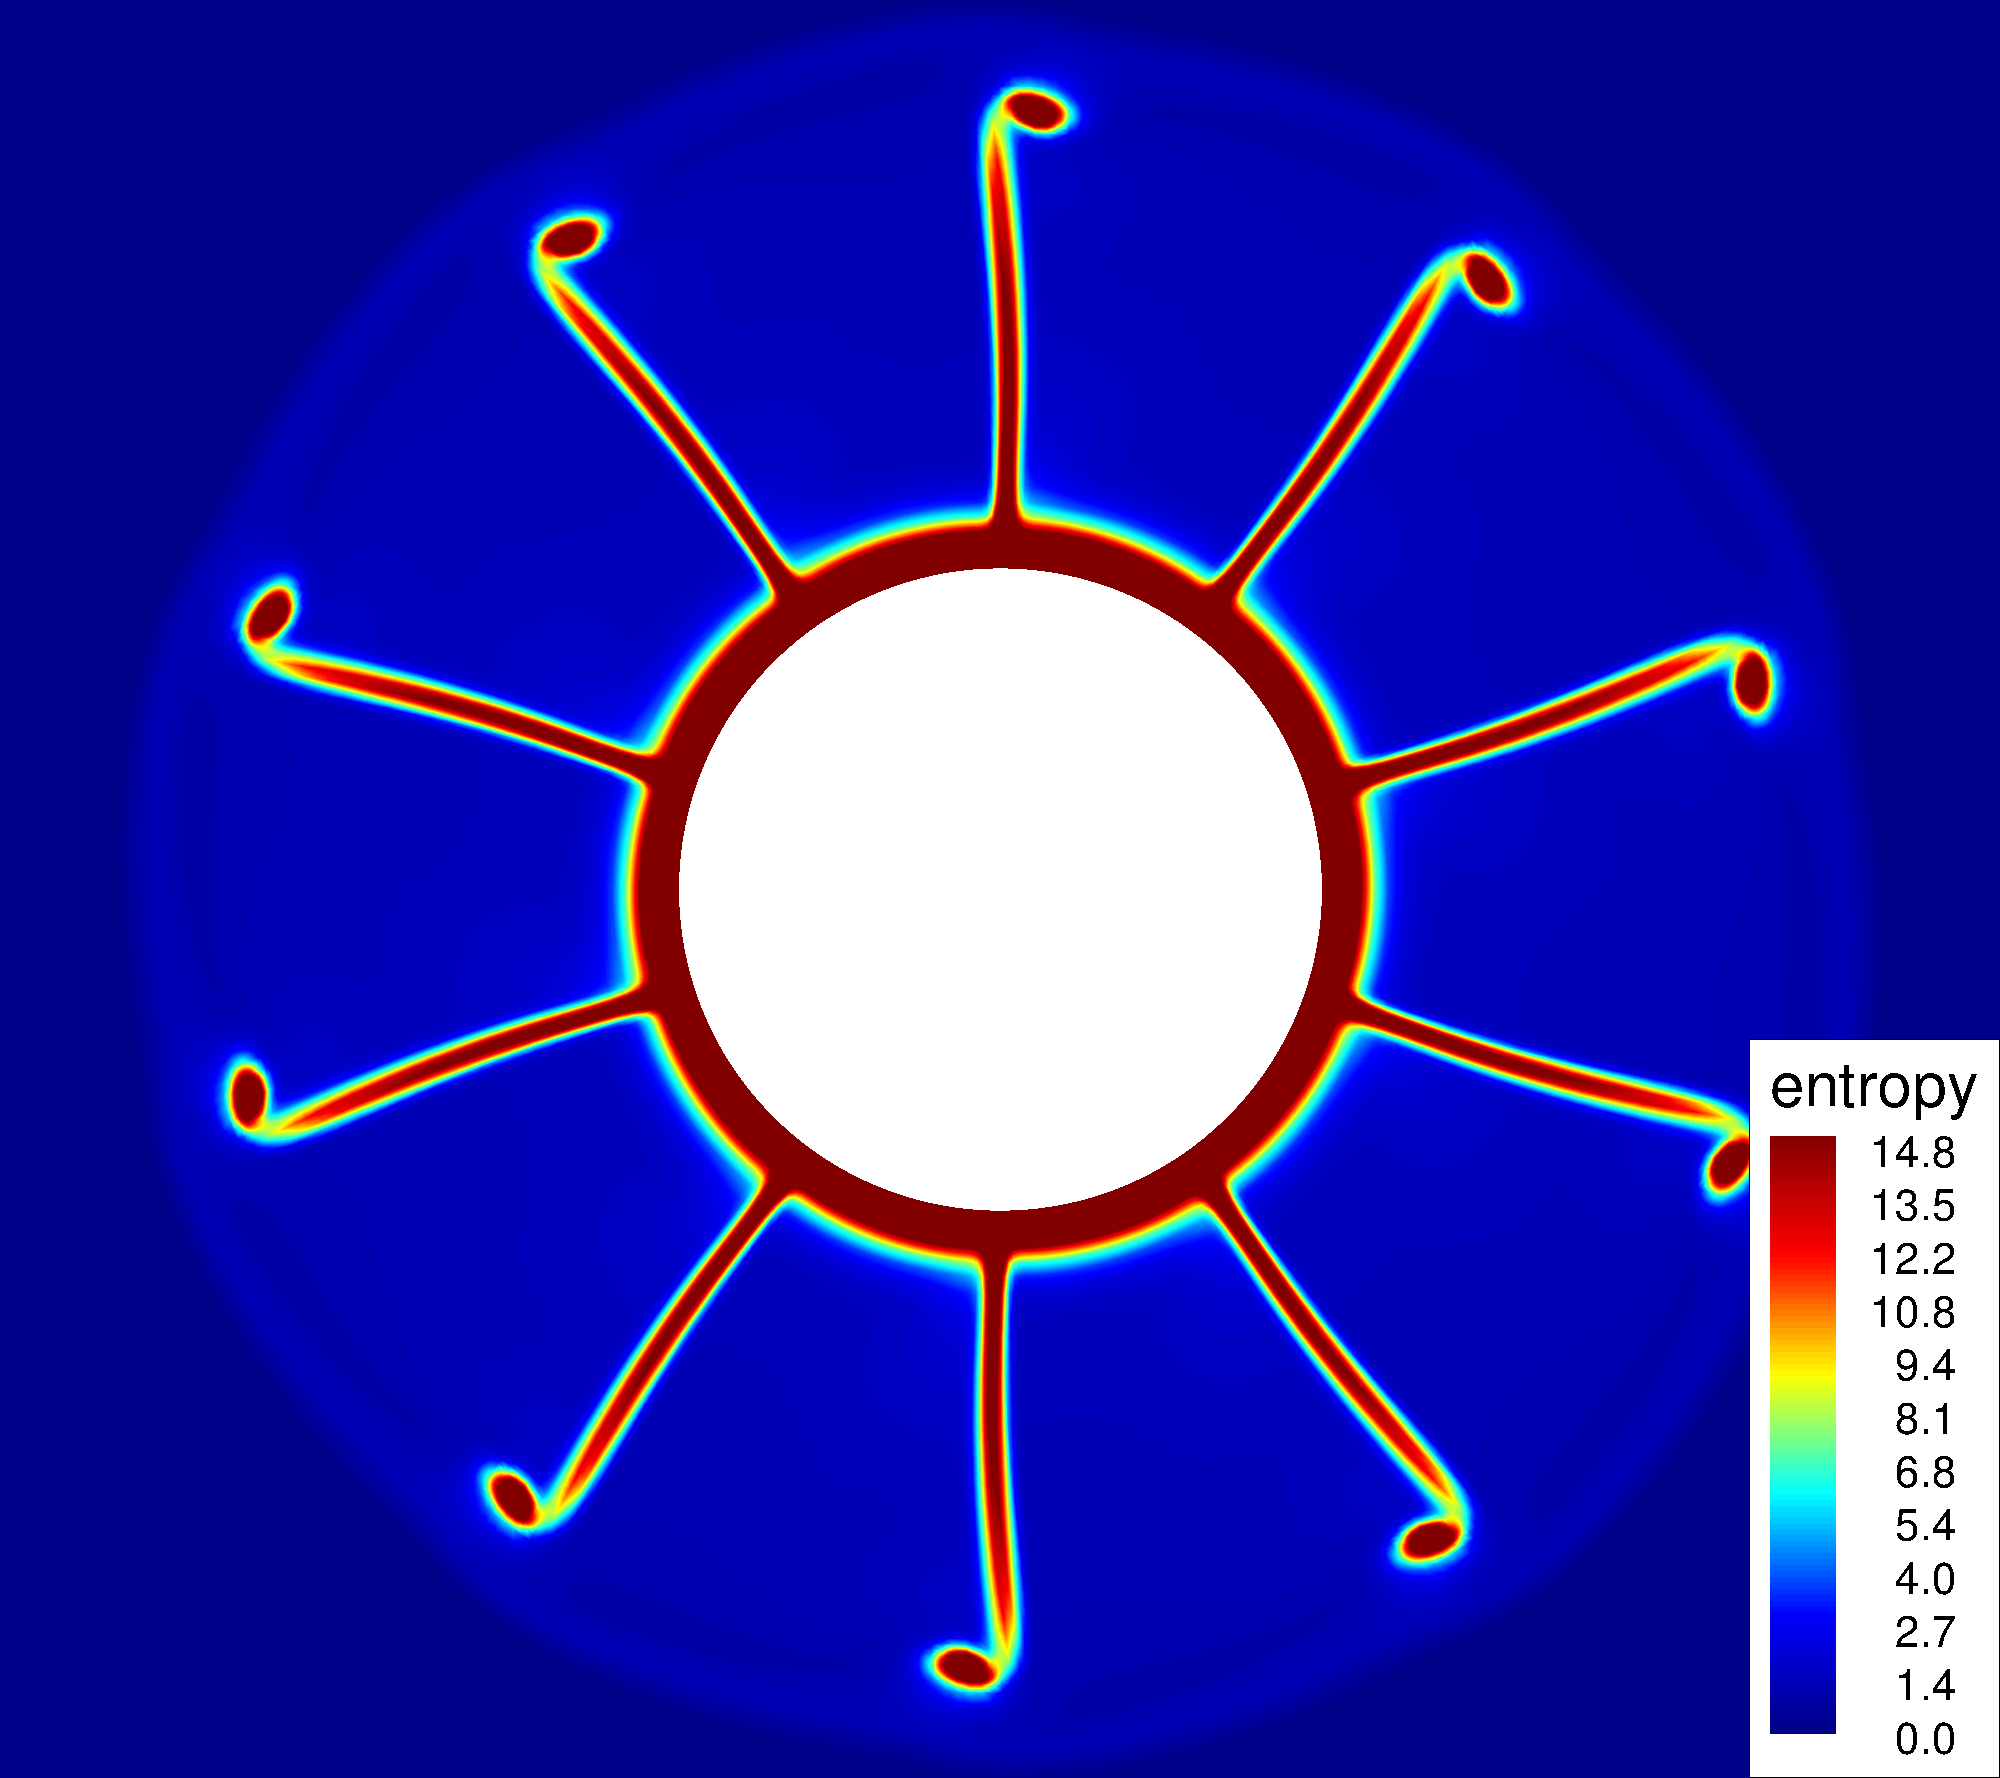
\includegraphics[width=.35\textwidth]{DREAM_HS_RANS_roe2_sa_slice_x_rear_2_entropy.png}
   & 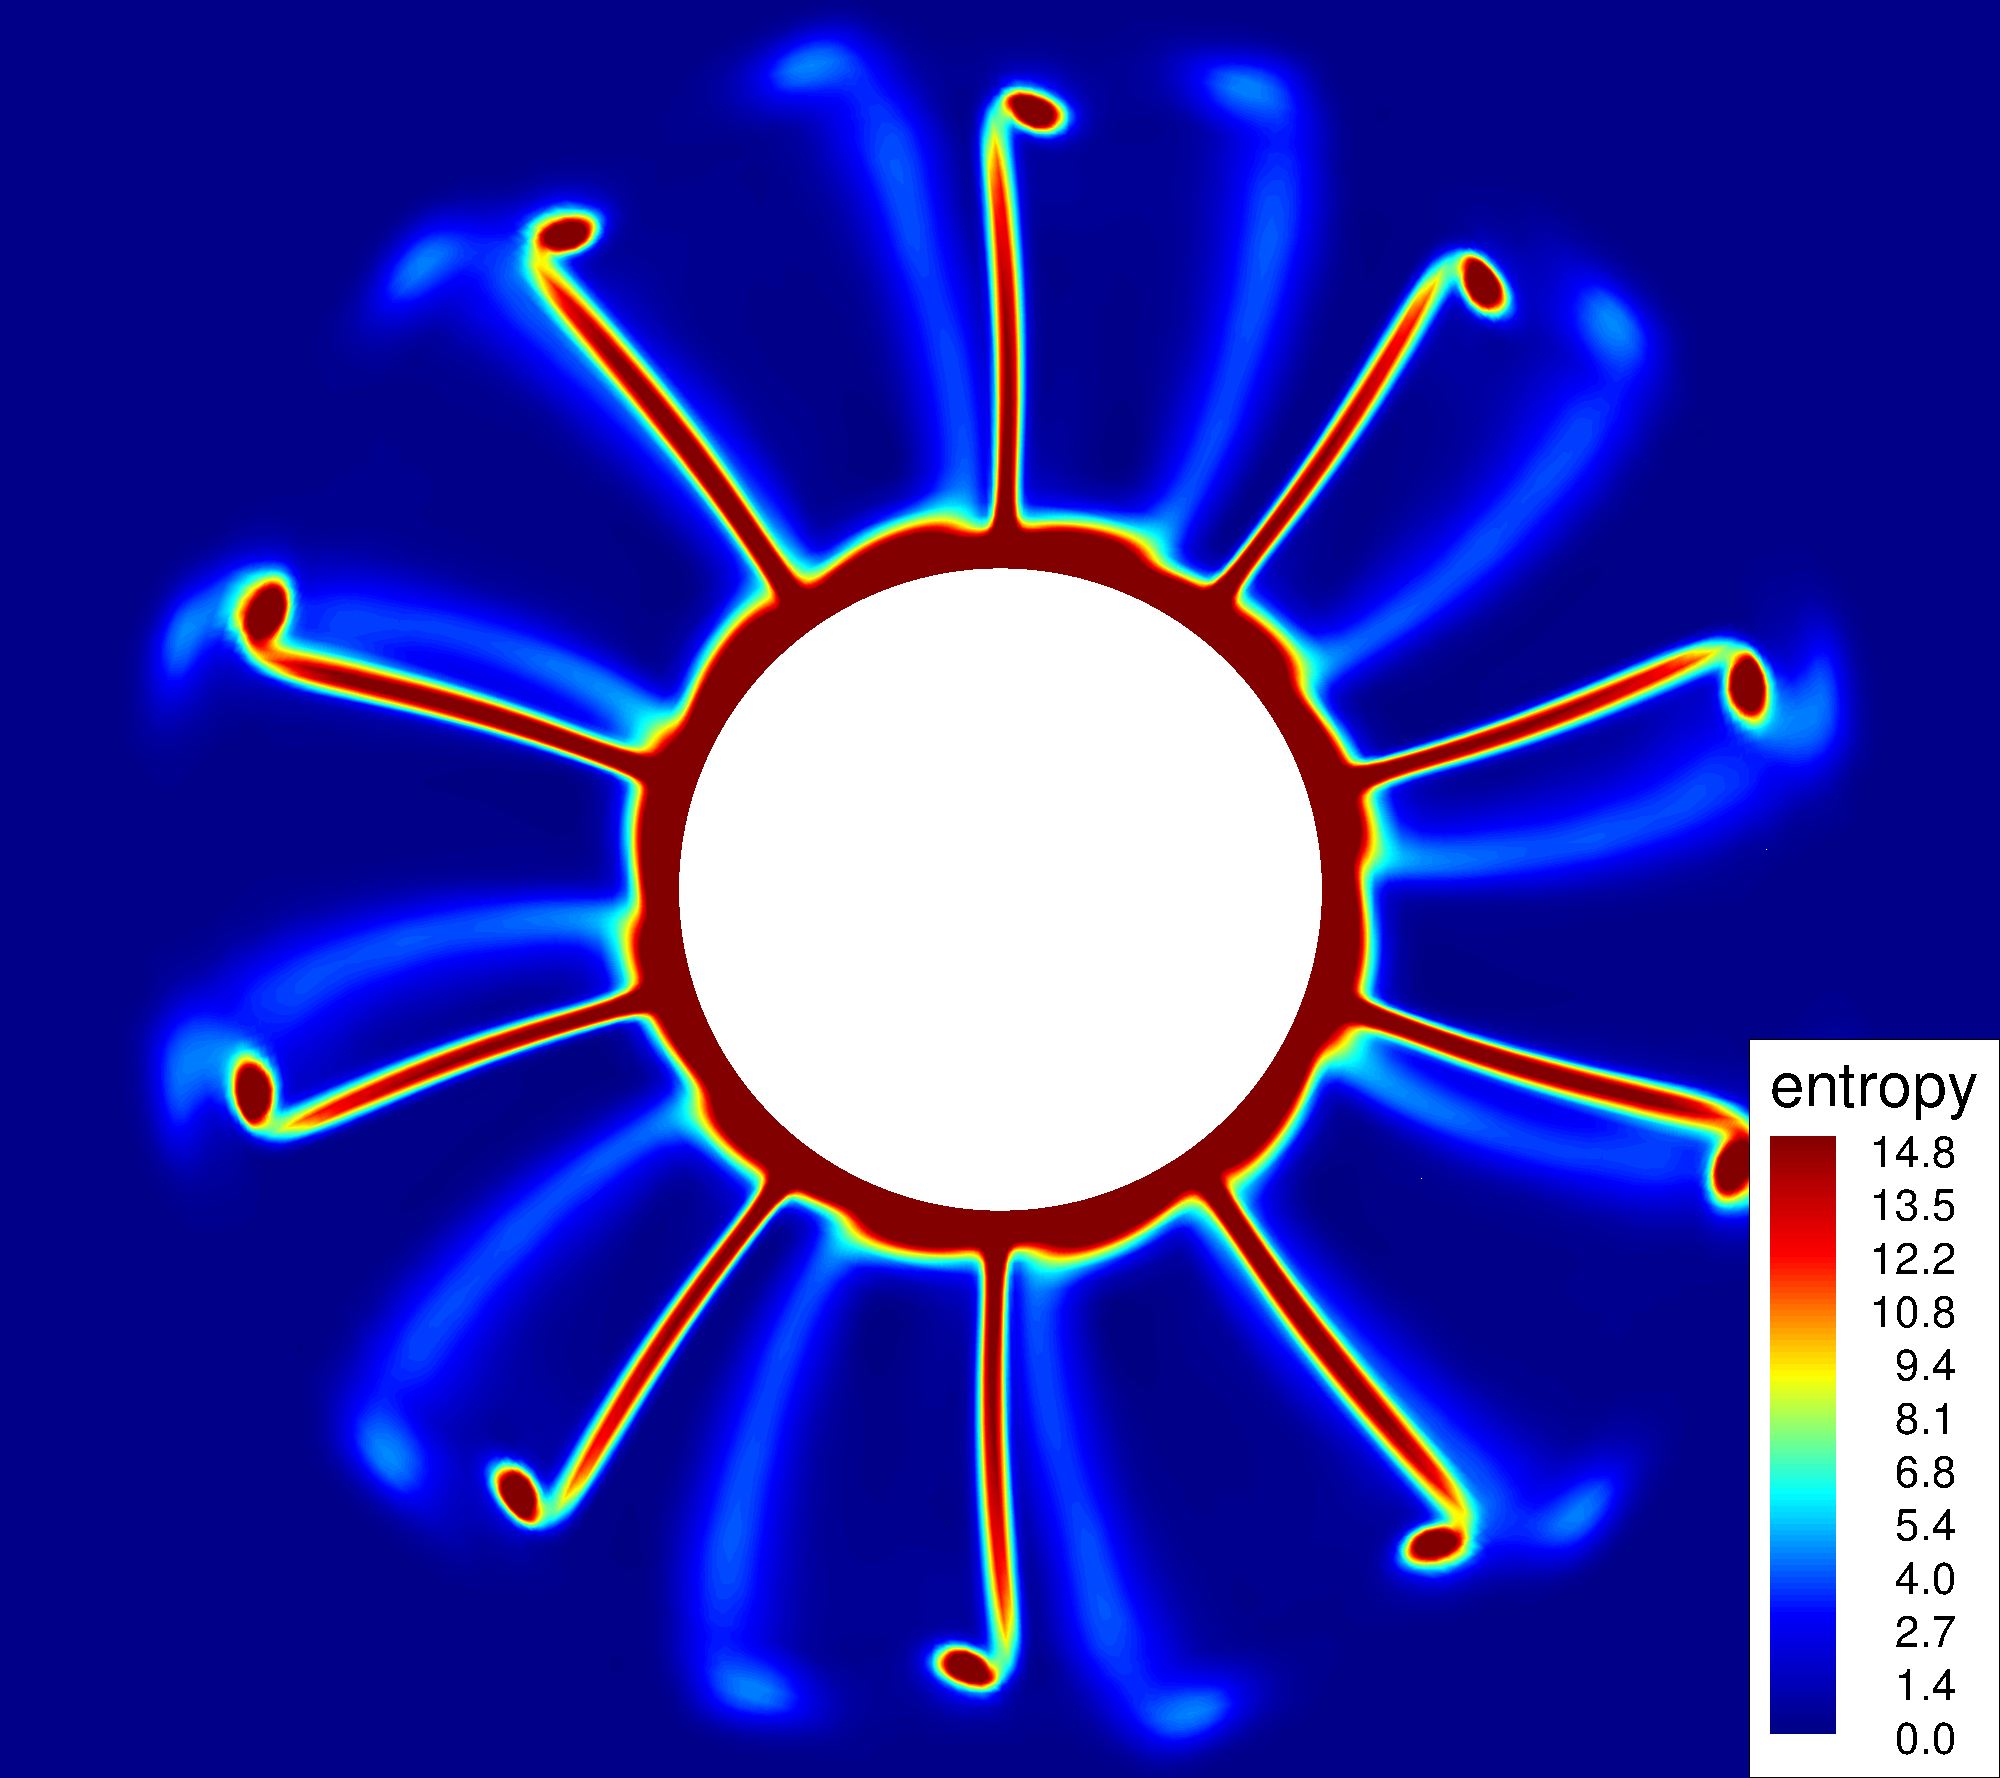
\includegraphics[width=.35\textwidth]{DREAM_HS_TSM_N7_roe2_sa_slice_x_rear_2_entropy.png} \\
 \end{tabular}
 \caption{High-speed isolated configuration: axial cuts of entropy.}
 \label{fig:dream_hs_hb_axial_cut_entropy}
\end{figure}
Clearly, the harmonic balance approach is able to transfer
the tangential distortions between the rows, allowing thus
to capture the interaction of the front tip vortices with
the rear rotor blades. In this high-speed configuration,
the front tip vortex does not hit the rear rotor blades.
The difference with the mixing plane approach is 
tremendous and justifies the use of an unsteady approach
over a steady one. 

One can see that the prediction tool has provided
the number of harmonics needed to ensure the continuity
of the tangential information at the rows interface.
In fact, at the $P4$ plane, no spurious entropy waves
are seen, giving us confidence in the unsteady results.

\subsection{Two-dimensional results: radial cut of harmonic pressure}
\label{sub:dream_hs_hb_radial_cuts}

\begin{figure}[htp]
  \centering
  \includegraphics*[width=0.40\textwidth]{DREAM_HS_TSM_N7_roe2_sa_slice_r_70_ps.png}
  \caption{High-speed isolated configuration: radial cut of the first harmonic of the
  static pressure normalized by the inflow static pressure.}
  \label{fig:dream_hs_hb_radial_cuts}
\end{figure}

\begin{figure}[htp]
  \centering
  \includegraphics*[width=0.40\textwidth]{DREAM_HS_TSM_N7_roe2_sa_slice_r_70_machrel.png}
  \caption{High-speed isolated configuration: radial cut of the first harmonic of the
  relative Mach number.}
  \label{fig:dream_hs_hb_radial_cuts_machrel}
\end{figure}

\section{Aeroelastic results}
\label{sec:dream_hs_ael_results}
%!TEX root = ../../../adrien_gomar_phd.tex

\subsection{Stability curve}
\label{sub:dream_hs_ael_curve}

The damping curves for the two modes of this high-speed
configuration are shown in Fig.~\ref{fig:dream_hs_ael_damping}.
The damping is positive for all the inter-blade phase angles
and modes, which clears this configuration for flutter.
In fact, the damping is around $2.1$ and $0.35$
for the torsional mode and the flection mode, respectively.
The torsional is much more damped than the flection one.
In opposite to the low-speed configuration, the 
variation range is similar for both modes. 
The minimum damping is obtained for IBPA=$30^\circ$
for the 2F mode and IBPA=$-30^\circ$ for the 1T mode.
To further analyze the aeroelastic behavior of the front rotor 
blades, the local damping is computed.
\begin{figure}[htp]
  \centering
  \subfigure[mode 2F]{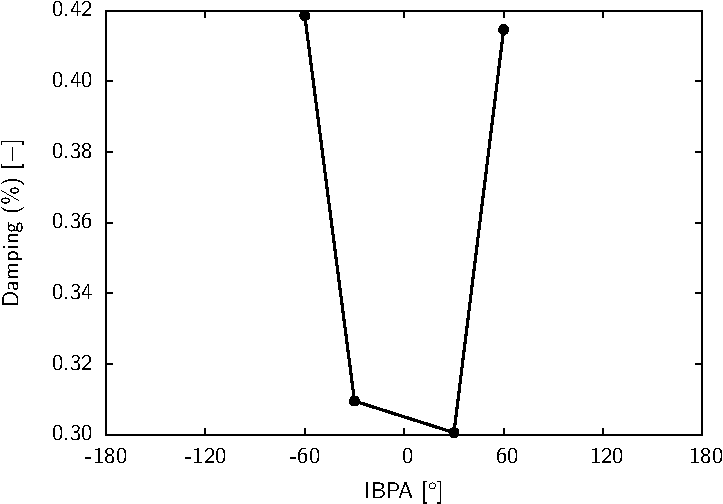
\includegraphics[width=.35\textwidth]{DREAM_HS_DAMPING_MODE_2F.pdf}}
  \subfigure[mode 1T]{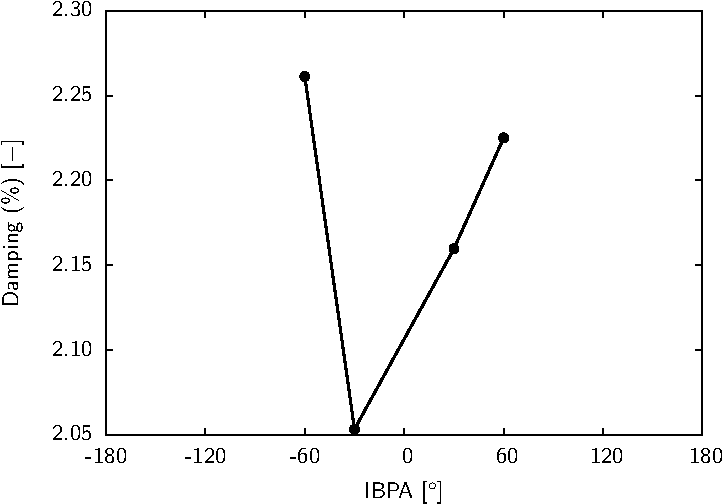
\includegraphics[width=.35\textwidth]{DREAM_HS_DAMPING_MODE_1T.pdf}}
  \caption{High-speed isolated configuration: integrated damping for modes 2F and 1T.}
  \label{fig:dream_hs_ael_damping}
\end{figure}

\subsection{Local excitation}
\label{sub:dream_hs_ael_local_damping}

The local excitation is shown on the pressure side and
the suction side of the front rotor blades in 
Figure~\ref{fig:dream_hs_ael_local_damping}. It is the
local damping given in each cell divided by the 
surface of the cell. It is therefore expressed in
m\textsuperscript{-2}.
\begin{figure}[htp]
 \ra{1.3} \centering
 \begin{tabular}{r|cccc}
   \toprule
   & \multicolumn{4}{c}{
        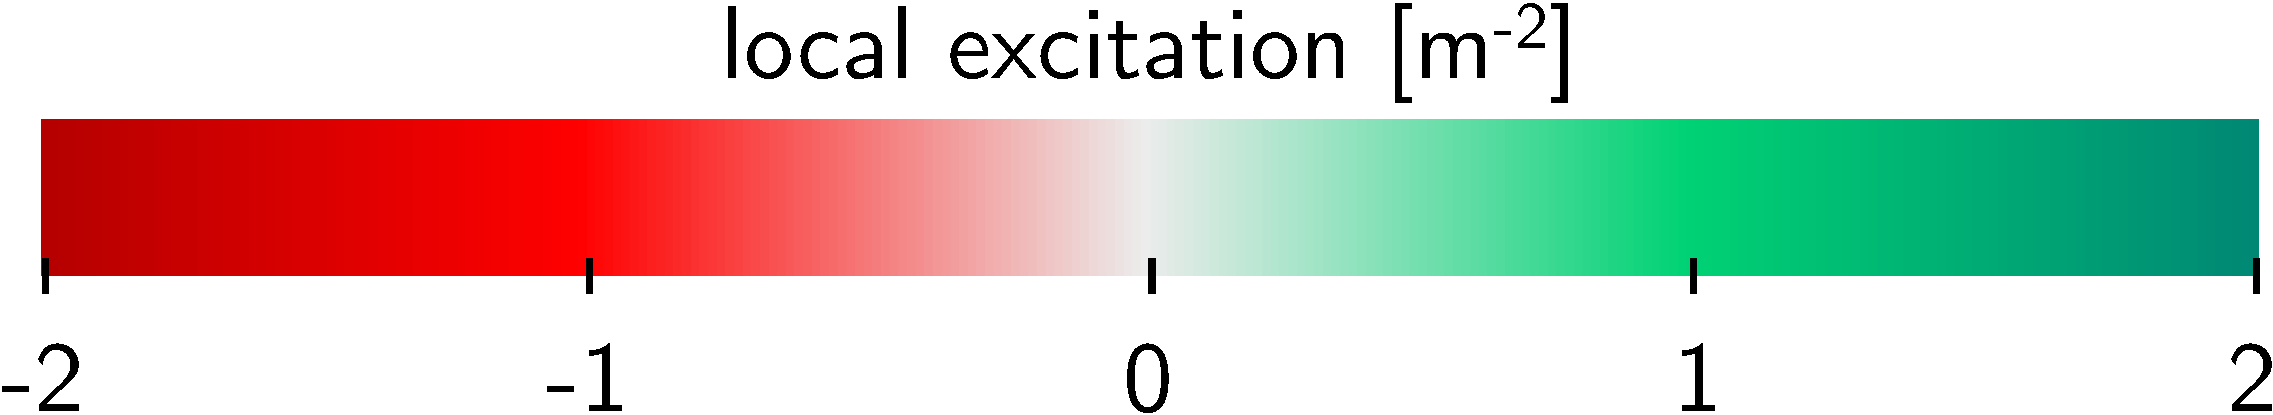
\includegraphics[width=0.22\textwidth]{dream_hs_damping_scale.pdf}} \\
   & \multicolumn{2}{c}{mode 2F} & \multicolumn{2}{c}{mode 1T} \\
   \midrule
   \rotatebox{90}{\quad\quad\quad IBPA $= -60^\circ$} 
   & 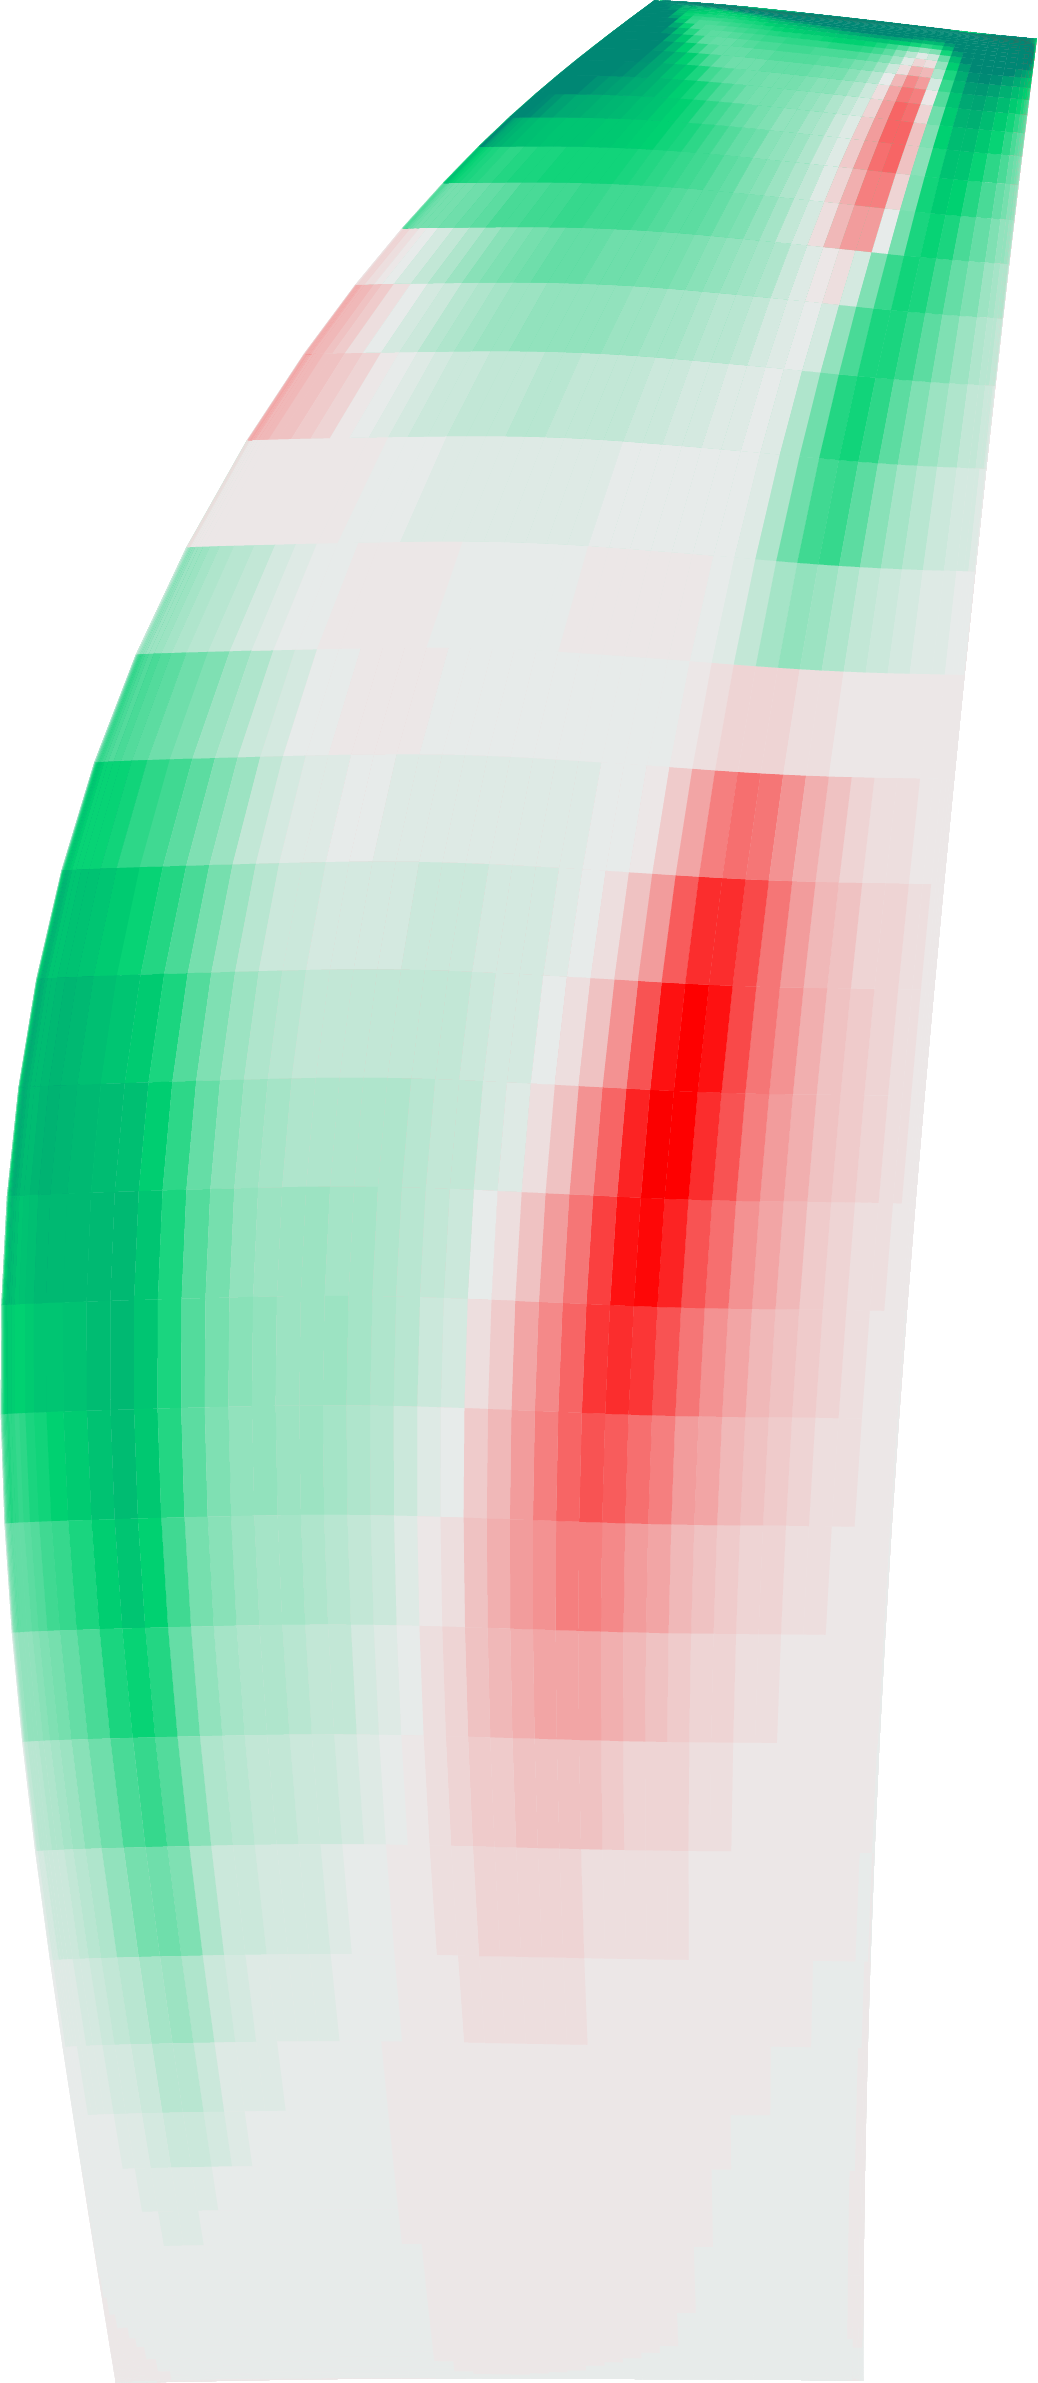
\includegraphics[width=0.12\textwidth]{DREAM_HS_HBT_N5_AEL_H1M2FD-3_roe3_sa_local_damping_SS.png}
   & 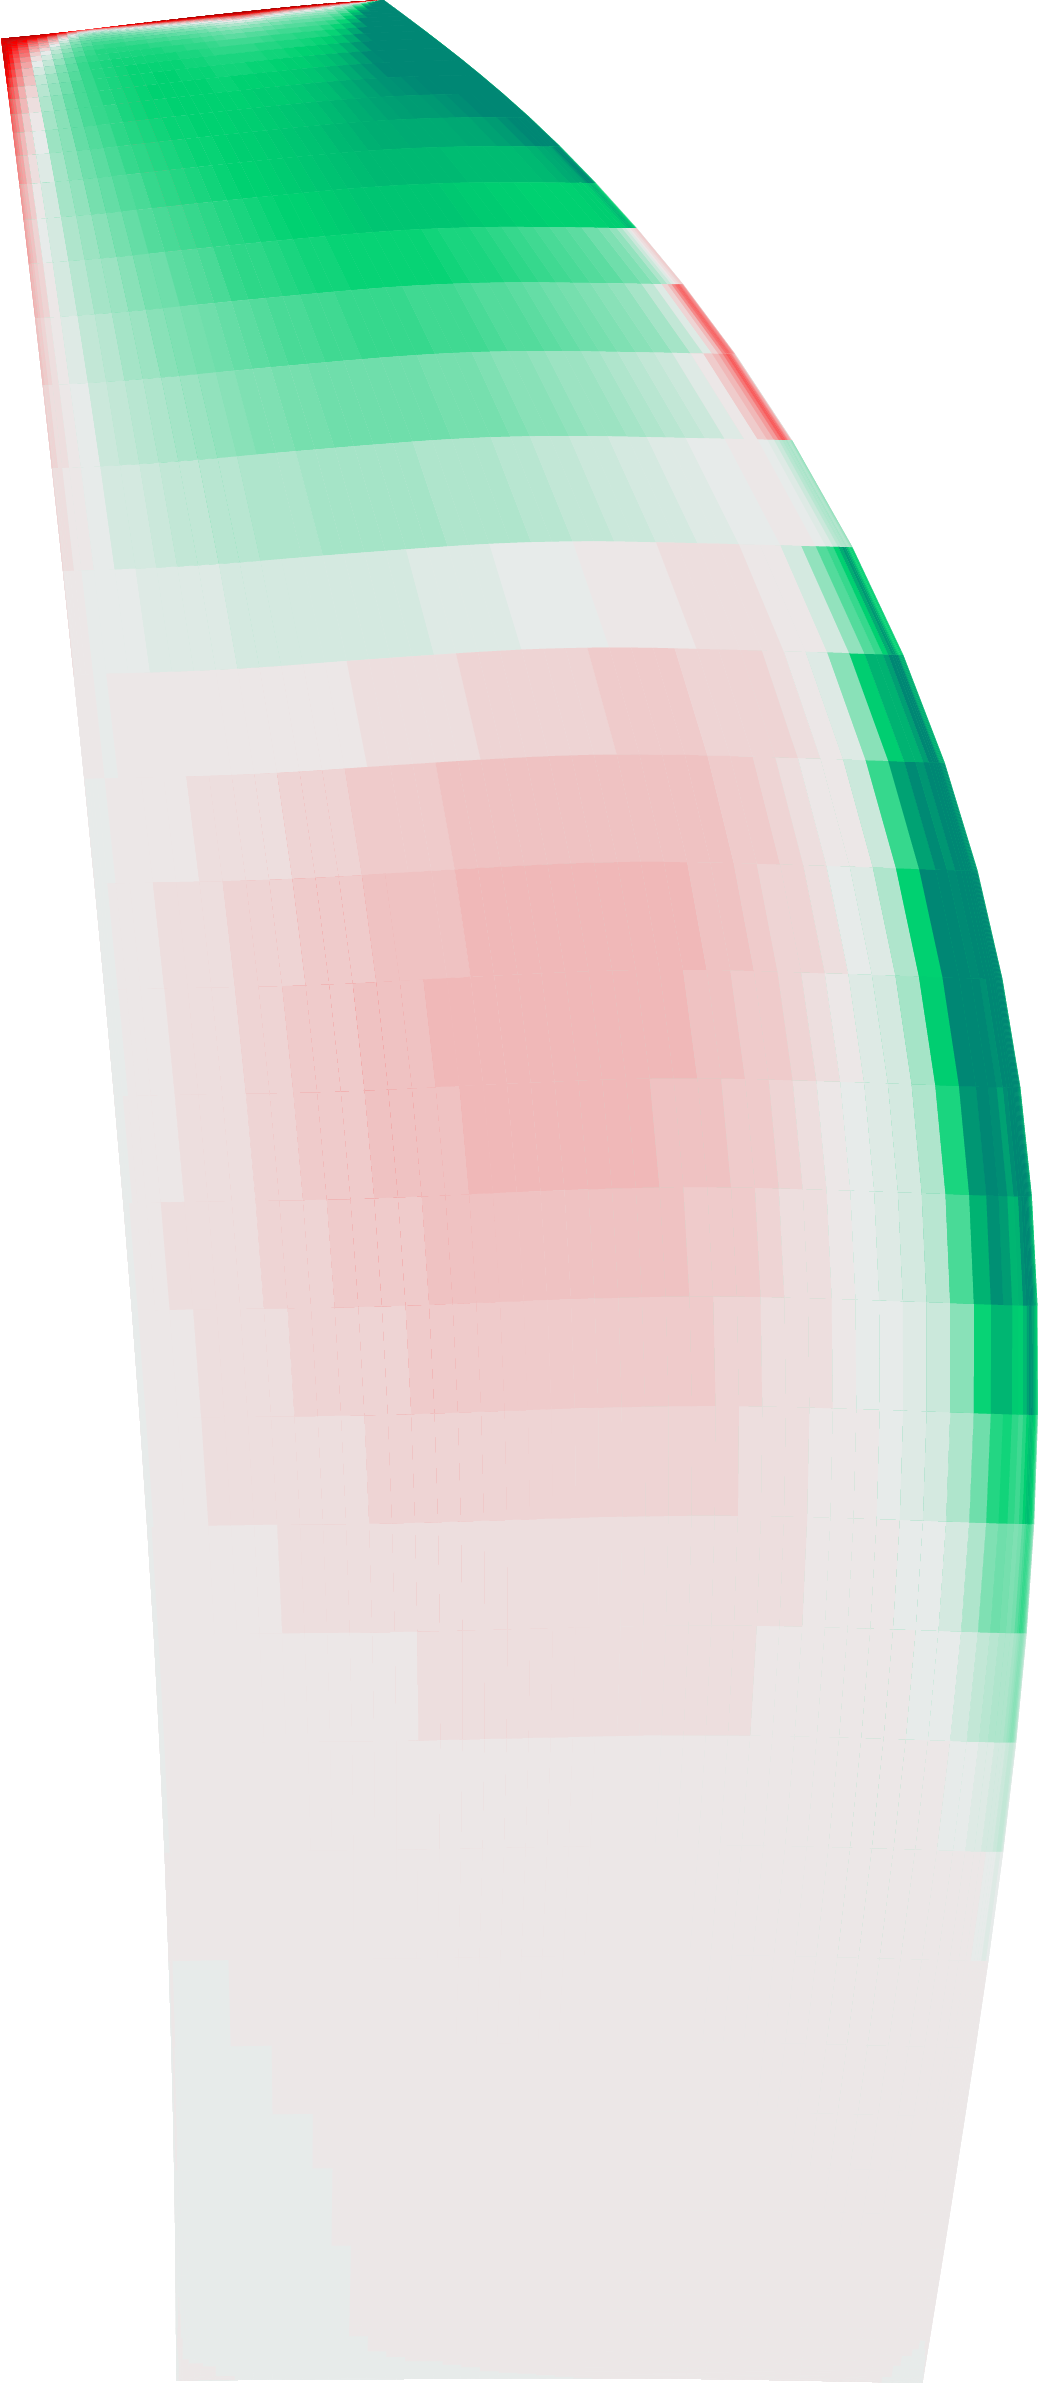
\includegraphics[width=0.12\textwidth]{DREAM_HS_HBT_N5_AEL_H1M2FD-3_roe3_sa_local_damping_PS.png}
   & \includegraphics[width=0.12\textwidth]{DREAM_HS_HBT_N5_AEL_H1M1TD-3_roe3_sa_local_damping_SS.png}
   & \includegraphics[width=0.12\textwidth]{DREAM_HS_HBT_N5_AEL_H1M1TD-3_roe3_sa_local_damping_PS.png} \\
   \rotatebox{90}{\quad\quad\quad IBPA $= -30^\circ$} 
   & \includegraphics[width=0.12\textwidth]{DREAM_HS_HBT_N5_AEL_H1M2FD-1_roe3_sa_local_damping_SS.png}
   & \includegraphics[width=0.12\textwidth]{DREAM_HS_HBT_N5_AEL_H1M2FD-1_roe3_sa_local_damping_PS.png}
   & \includegraphics[width=0.12\textwidth]{DREAM_HS_HBT_N5_AEL_H1M1TD-1_roe3_sa_local_damping_SS.png}
   & \includegraphics[width=0.12\textwidth]{DREAM_HS_HBT_N5_AEL_H1M1TD-1_roe3_sa_local_damping_PS.png} \\
   \rotatebox{90}{\quad\quad\quad IBPA $= 30^\circ$} 
   & \includegraphics[width=0.12\textwidth]{DREAM_HS_HBT_N5_AEL_H1M2FD1_roe3_sa_local_damping_SS.png}
   & \includegraphics[width=0.12\textwidth]{DREAM_HS_HBT_N5_AEL_H1M2FD1_roe3_sa_local_damping_PS.png}
   & \includegraphics[width=0.12\textwidth]{DREAM_HS_HBT_N5_AEL_H1M1TD1_roe3_sa_local_damping_SS.png}
   & \includegraphics[width=0.12\textwidth]{DREAM_HS_HBT_N5_AEL_H1M1TD1_roe3_sa_local_damping_PS.png} \\
   \rotatebox{90}{\quad\quad\quad IBPA $= 60^\circ$} 
   & \includegraphics[width=0.12\textwidth]{DREAM_HS_HBT_N5_AEL_H1M2FD3_roe3_sa_local_damping_SS.png}
   & \includegraphics[width=0.12\textwidth]{DREAM_HS_HBT_N5_AEL_H1M2FD3_roe3_sa_local_damping_PS.png}
   & \includegraphics[width=0.12\textwidth]{DREAM_HS_HBT_N5_AEL_H1M1TD3_roe3_sa_local_damping_SS.png}
   & \includegraphics[width=0.12\textwidth]{DREAM_HS_HBT_N5_AEL_H1M1TD3_roe3_sa_local_damping_PS.png} \\
   & suction side & pressure side & suction side & pressure side \\
   \bottomrule
 \end{tabular}
 \caption{High-speed isolated configuration: local excitation for modes 2F and 1T.}
 \label{fig:dream_hs_ael_local_damping}
\end{figure}

Firstly, the level of local excitation is larger for the
1T mode than it is for the 2F mode. This is one explication
for the difference in damping amplitude observed above.
This can be attributed again to the displacement related to the
1T mode. In fact, this mode has the tendency to change the
local angle of attack of the blade, yielding an unadapted
inflow velocity. This angle of attack drives, for the most part,
the aerodynamic behavior around the blade. Therefore, a small
change in angle of attack can have a strong impact on the loading and
the local excitation might be emphasized.
Compared to the low-speed configuration, the local excitation
is always positive on the leading edge of the blade, meaning
that the change in angle of attack and in dihedral angle
produces for the torsional and the flection mode, respectively,
is a positive feature for the damping.

Secondly, the influence of the IBPA remains limited for the
two modes. The global phenomenology is
kept unchanged even though the amplitude varies.
For the torsional mode, the local excitation of
the tip of the blade seems to be sensitive 
to the IBPA. This is the tip vortex region, and
advanced post-processing procedures might be required
to fully understand the behavior of local excitation
near the tip of the blades.

Globally the shape of the local excitation contours
is much more complicated on the high-speed configuration
compared to the low-speed one. In fact, 
not only the modes inflection lines become inflection lines
for the local excitation, but also the shock and 
the flow that develops in the tip region are important.

\subsection{Influence of the number of harmonics on the aeroelastic results}
\label{sub:dream_hs_convergence_ael}

To assess the convergence of the capture of the damping by the multi-frequential
HB approach, four computations are run on the second flection mode
of the high-speed CROR configuration. For each computation, the 
vibration frequency is considered with one to several harmonics
of the blade passing frequency of the rear rotor. As indicated in
Sec.~\ref{par:choice_of_frequencies}, several approaches exist to
truncate the frequency sets. Here, only the "cross grid" truncation 
pattern is used with only one aeroelastic frequency.
\begin{figure}[htp]
 \ra{1.3} \centering
 \begin{tabular}{r|cccc}
   \toprule
   & \multicolumn{4}{c}{
        \includegraphics[width=0.22\textwidth]{dream_hs_damping_scale.pdf}} \\
   & $N=2$ & $N=3$ & $N=4$ & $N=5$ \\
   \midrule
   \rotatebox{90}{\quad\quad\quad suction side} 
   & \includegraphics[width=0.12\textwidth]{DREAM_HS_HBT_N2_AEL_H1M2FD-1_roe3_sa_local_damping_SS.png}
   & \includegraphics[width=0.12\textwidth]{DREAM_HS_HBT_N3_AEL_H1M2FD-1_roe3_sa_local_damping_SS.png}
   & \includegraphics[width=0.12\textwidth]{DREAM_HS_HBT_N4_AEL_H1M2FD-1_roe3_sa_local_damping_SS.png}
   & \includegraphics[width=0.12\textwidth]{DREAM_HS_HBT_N5_AEL_H1M2FD-1_roe3_sa_local_damping_SS.png} \\
   \rotatebox{90}{\quad\quad\quad pressure side} 
   & \includegraphics[width=0.12\textwidth]{DREAM_HS_HBT_N2_AEL_H1M2FD-1_roe3_sa_local_damping_PS.png}
   & \includegraphics[width=0.12\textwidth]{DREAM_HS_HBT_N3_AEL_H1M2FD-1_roe3_sa_local_damping_PS.png}
   & \includegraphics[width=0.12\textwidth]{DREAM_HS_HBT_N4_AEL_H1M2FD-1_roe3_sa_local_damping_PS.png}
   & \includegraphics[width=0.12\textwidth]{DREAM_HS_HBT_N5_AEL_H1M2FD-1_roe3_sa_local_damping_PS.png} \\
   \bottomrule
   \multicolumn{1}{c}{}& \\
   \multicolumn{1}{c}{} & \multicolumn{4}{c}{
        \includegraphics[width=0.45\textwidth]{DREAM_HS_COMVERGENCE_DAMPING.pdf}} \\
 \end{tabular}
 \caption{High-speed isolated configuration: convergence of local excitation and damping.}
 \label{fig:dream_hs_ael_convergence_damping}
\end{figure}
The local excitation and damping results are 
shown in Fig.~\ref{fig:dream_hs_ael_convergence_damping}.
Raising the number of harmonics of the rear rotor blade passing frequency
changes the damping by at-most 10\% but the contours
of the local excitation are kept nearly unchanged. Only small differences
are observed, that integrated produces the 10\%
observed on the damping value. Further investigation of the
convergence for the choice of frequencies are needed, but
this has not been done on this work.


\chconclu{The multi-frequential harmonic balance
method along with a weak-coupling approach has been
assessed on a high-speed CROR configuration.
The steady computations reveal strong non-linear 
features, namely shocks. The prediction tool
defined in Chap.~\ref{cha:limitations_convergence}
is then used to estimate the number 
of harmonics required to simulate the configuration.
Seven harmonics are needed for the high-speed configuration
whereas only four were required for the low-speed one
for the same accuracy.
No intermediate simulation is launched and the results
are shown to be consistent, namely tip vortex and wakes interactions
are captured. 
Aeroelastic simulations are then launched.
The results are finally assessed by post-processing the integrated damping
and the local excitation of the blades.
This configuration is also shown to be flutter free.
The proposed methodology is thus demonstrated to be able to
tackle demanding industrial configurations.}
